% Paper notes: the source of the notes map (pixi run notes-map) and of a PDF
% (pixi run build-notes). Run pixi run notes-check before you commit.
%
% A programme, with its papers inside it:
%
%   \begin{programnote}{Group -- what they build}{Key}
%   \location{lat}{lon}{City, Country}   % the map pin
%   \thumb{img/key.png}                  % optional; images live in img/
%   \paragraph{What it is}
%   ...
%   \begin{confnote}{IEEE NSS/MIC 2027 -- Pasadena}{NSSMIC2027}
%   \dates{2027-10-30}{2027-11-06}       % a conference: dates, and the map
%   \deadline[abstracts]{2027-05-12T23:59:59+02:00}   % counts down to this
%   \end{confnote}
%
%   \begin{papernote}{Author et al.\ Year -- Title}{AuthorYear}
%   Journal vol:page, \doi{10.xxxx/...}.  % or \href{url}{name}: the card's link
%   \paragraph{Summary}
%   ...
%   \end{papernote}
%   \end{programnote}
%
% Rules:
%  - Put each \begin and \end on its own line.
%  - Keep the title format. The year dates and orders the cards, and the text
%    before " -- " is the name a \ref{prog:Key} or \ref{note:Key} shows.
%  - A paper's key is its references.bib key (AuthorYear, a/b for a second
%    paper), which also names its PDF, papers/<Key>.pdf. A programme's key is
%    a short name; notesmap.toml lays the board out by it.
%  - Cards in the Ideas programme are experiment ideas, not papers: keys start
%    with Idea and they carry no year.
%  - An image is img/<key in lower case>.png; a second one adds a suffix,
%    img/freire2026-table2.png.
%  - A paper outside any programme is a top-level papernote, and the map
%    leaves it out.
%
% The map is public. The PDF keeps everything.
%  - Shown on the map: What it is, Summary, Detector, Method, Key Findings,
%    People, and any heading not listed under [publish] in notesmap.toml.
%  - Hidden from the map: Why it matters here, Capsule, Relevance to This
%    Thesis, Where It Might Go, Thesis entry, Scope boundary. Put your own
%    reasoning under these headings.
%  - \aside{...} marks a remark of your own inside a shown paragraph.
%  - \gap{...} marks something not yet checked. The map hides it.
%  - A \ref inside hidden text draws no arrow.
%
% More detail is in tools/notesmap/README.md.

\documentclass[11pt, a4paper]{article}

\usepackage[margin=2.5cm]{geometry}
\usepackage{amsmath, amssymb}
\usepackage[backend=biber, style=numeric, sorting=none]{biblatex}
\usepackage{siunitx}
% units.tex and references.bib are the thesis's own, found via the
% -Z search-path=src/thesis that build-notes passes. No copies to keep in sync.
\input{units} % \keV{511} etc.
% a \pm inside a number prints as "1.38 ± 0.23 mm", not siunitx's default
% "1.38(23) mm" -- the map spells it out and the PDF should match.
\sisetup{separate-uncertainty=true}
\usepackage{xcolor}
\usepackage[hidelinks]{hyperref}
\usepackage{xurl}
% programnote/papernote, \location, \thumb, \doi, \gap: the macros the
% notes map reads (tools/notesmap; the canonical copy is in its templates/)
\usepackage{notesmap}

\addbibresource{references.bib}

% As in main.tex: block (not run-in) \paragraph.
\usepackage{titlesec}
\titleformat{\paragraph}[block]{\normalfont\bfseries\raggedright}{}{0pt}{}
\titlespacing*{\paragraph}{0pt}{1.5ex plus 1ex minus .2ex}{0.5ex}

\begin{document}

\tableofcontents

\clearpage

\begin{programnote}{UTOFPET -- Pisa + Ghent monolithic TOF-PET}{UTOFPET}
\location[-68,109]{43.72}{10.40}{Pisa, Italy}

\paragraph{What it is}
A joint project of the University of Pisa (Dipartimento di Fisica E.\ Fermi /
INFN Pisa) and Ghent University (MEDISIP), named explicitly in the WT-PET design
paper as the origin of the WT-PET detector. EPFL (Bruschini, Charbon, Gramuglia)
appears on the consortium's flagship instrumentation paper.
\gap{Funding source, grant number, start and end dates. Determines whether the
follow-up agenda is live or concluded --- materially changes how much of the
surrounding space should be treated as spoken for.}

\paragraph{Why it matters here}
Three separate entries on the prior-art kill list resolve to this single actor.
Carra et al.\ 2022 (\ref{note:Carra2022}) and the Ghent monolithic lineage
(Stockhoff 2021, Decuyper 2021, Maebe 2022) are not independent groups arriving
at similar results; they are one programme with a shared detector. Treat the
consolidated entity as the wall, and its scope boundary as the map.

\paragraph{Detector lineage}
The scaling is worth stating plainly:

\begin{itemize}
	\item \textbf{Preclinical / Pisa:} \qtyproduct{25.6 x 25.6 x 8}{\milli\metre}
		LYSO monolith, 64 Hamamatsu S14160-3050 SiPMs at \mm{3.2} pitch.
		\mm{0.78} 2D FWHM, \mm{1.55} DOI FWHM, \ps{156} CTR at one
		operating point (\ref{note:Carra2022}).
	\item \textbf{Preclinical / Ghent:} the $\beta$-CUBE
		(\ref{note:Krishnamoorthy2018}), \qtyproduct{25.4 x 25.4 x 8}{\mm}
		LYSO. This, not the Pisa block, is reference [18] in the WT-PET paper,
		the detector ``scaled up by a factor of 2''; Pisa's development is cited
		separately ([22], \ref{note:Carra2022}).
	\item \textbf{Clinical block, measured:} Stockhoff et al.\ 2021
		(\ref{note:Stockhoff2021}) is the doubled block itself ---
		\qtyproduct{50 x 50 x 16}{\mm} LYSO on 8 x 8
		\qtyproduct{6 x 6}{\mm} SiPMs with 6-layer DOI --- not a parallel
		design.
	\item \textbf{Clinical / WT-PET:} \qtyproduct{50 x 50 x 16}{\milli\metre}
		BGO or LYSO, 8 x 8 array of \qtyproduct{6 x 6}{\milli\metre} SiPMs,
		6-layer DOI. The WT-PET paper states the detector was developed in
		UTOFPET and that thickness and transverse size were taken from existing
		preclinical monolithic detectors ``scaled up by a factor of 2''.
\end{itemize}

Every dimension roughly doubles, and the SiPM pitch with it (\mm{3.2}
$\rightarrow$ \mm{6}), preserving the 8 x 8 channel count. \textbf{The clinical
block geometry was set by doubling a prototype, not by optimisation} --- stated
in their own words. \aside{Note this: it is a clean, citable instance of design-by-scaling
in exactly the place a co-design argument wants one.}

\paragraph{WT-PET system context (Vandenberghe et al.\ 2023, EJNMMI 50(12):3558--3571)}
Two flat panels, each \qtyproduct{70 x 106}{\centi\metre}, \cm{50} apart, patient
standing upright between them. 14 x 20 = 280 monolithic blocks per panel.
Detector surface reduced 1.9x and scintillator volume 2.2x versus LAFOV systems
at comparable sensitivity. Its simulations give spatial resolution below
\mm{2} across the whole imaging volume and NEMA sensitivity
\qty{152}{kcps\per\mega\becquerel} with BGO (114 with LYSO) against 176.0 for
the Quadra (its Table 4). Ghent-led;
Sportelli and Belcari (Pisa) are co-authors. Carra is not on this paper.

\aside{These system numbers are context only --- they do not belong in any chapter of
this thesis. The detector spec above does.}

\paragraph{Intellectual property}
Italian patent application \textbf{102021000026609}, ``Method and device for the
acquisition of gamma photons through neural networks'', deposited at UIBM,
cited alongside the consortium's 2021 NSS/MIC paper.

\textbf{Action:} pull the claim text from Espacenet or the UIBM register.
Published papers show what has been \emph{done}; claims show what has been
\emph{fenced}, and a broadly drafted claim on NN-based gamma acquisition could
reach arrival-time-based cardinality inference even though no paper runs it.
This should be checked before committing the temporal axis as a surviving
direction.

\paragraph{Scope boundary --- what they have \emph{not} claimed}
Useful precisely because it is narrow and legible:
\begin{itemize}
	\item Monocrystalline LYSO and BGO. Nothing on nanocomposite or ceramic
		scintillators, or Rayleigh-dominated media.
	\item Flat-panel and cylindrical clinical geometry. Nothing annular at
		preclinical scale.
	\item Single-vertex estimation. No cardinality, no interaction ordering,
		no multi-vertex separability. \gap{Verify against the most recent
		consortium output, not just the 2022 paper.}
	\item Demonstration, not characterisation. No Fisher information, no CRLB,
		no bound of any kind anywhere in the lineage.
	\item Detector geometry as a fixed input. The WT-PET block was sized by
		doubling; nothing in the programme treats detector parameters as
		optimisation variables.
\end{itemize}

\paragraph{People}
Pisa: Belcari (senior), Bisogni, Sportelli, Carra, Ciarrocchi, Morrocchi, Rosso.
Ghent: Vandenberghe (PI, WT-PET), Van Holen, Stockhoff, Decuyper, Maebe.
EPFL: Charbon, Bruschini, Gramuglia.
Carra co-authors directly with Vandenberghe, Van Holen and Stockhoff on the 2021
NSS/MIC paper ``Towards the ideal PET detector: a scalable architecture with high
intrinsic spatial resolution, DOI and sub-\ps{200} TOF capability'' --- the
personal link, not merely an institutional one.

\begin{papernote}{Carra et al.\ 2022 -- Simultaneous NN event positioning and timestamping in monolithic scintillators}{Carra2022}
\thumb{img/carra2022.png}
Phys.\ Med.\ Biol.\ 2022, \doi{10.1088/1361-6560/ac72f2}.

\paragraph{Summary}
Pisa (Dipartimento di Fisica E.\ Fermi, Università di Pisa; INFN Sezione di
Pisa). All seven authors --- Carra, Bisogni, Ciarrocchi, Morrocchi, Sportelli,
Rosso, Belcari --- share those two affiliations; no Ghent affiliation appears on
this paper despite the consortium relationship (\ref{prog:UTOFPET}).

Method proceeds in two stages: an event timestamping algorithm based on neural
networks, which is then integrated into a second network performing simultaneous
position and timestamp estimation. Validated first in simulation, then on
experimentally acquired data. The abstract says both algorithms are
implemented in a low-cost FPGA; the body names no FPGA and reports no measured
resources or latency, only an estimate (10--90\% of a medium-sized FPGA) and
training on a GPU. The simulation is in-house, on Geant4 with the LUT Davis
reflection model and custom SiPM Monte Carlo --- not GATE.

\paragraph{Capsule}
Carra et al.\ \cite{Carra2022} train a neural network that estimates event position
\emph{and} timestamp jointly from a monolithic LYSO block, and --- the actual
contribution --- design it light enough to run on a low-cost FPGA inside the
detector at more than $10^{6}$ events per second (claimed, not demonstrated in
the body). Reported on experimental data at a 12 V
overvoltage (Table 9, in the crystal corners by §3.4, though the same section
also calls the 2D figure an average): \mm{0.78} 2D FWHM in $(x,y)$, \mm{1.55}
DOI FWHM,
\ps{156} CTR, on a
\qtyproduct{25.6 x 25.6 x 8}{\milli\metre} LYSO monolith read out by 64
\qtyproduct{3 x 3}{\milli\metre} Hamamatsu SiPMs. The paper's stated framing is
that monolithic crystals plus light networks can rival pixellated performance for
TOF-PET while retaining better spatial and DOI resolution, with on-line
characterisation solving the scalability and computational-complexity objection
that had kept monolithics out of clinical scanners.
Energy resolution is 11\% at 511 keV at the same overvoltage (10\% lower down;
Table 9 and Fig.\ 11).
\aside{The abstract's \mm{1.2} DOI is from 3 V, where the CTR is \ps{290}; its
\ps{156} is from 12 V, where the DOI is \mm{1.55}. No one setting gives both:
positioning wants a low overvoltage and timing a high one (their Fig.\ 7). The
map uses 12 V throughout.}
The CTR is measured against a pixelated reference of about \ps{130}, removed in
quadrature and scaled by $\sqrt{2}$ to two identical monoliths, so it is not
flagged r; and the best figures need simulated events in the training set ---
on experimental data alone, \ps{194} and \mm{0.88} at the same overvoltage.

Two things matter here beyond the numbers. First, the WT-PET paper cites this
as the UTOFPET detector development behind its clinical block (see
\ref{prog:UTOFPET}), though the preclinical detector it says it scaled by two is
the $\beta$-CUBE. Second,
this is the paper that closes the naive form of ``use a network for position and
time together,'' and it argues for deployment, not just the algorithm.

\paragraph{Key Findings}
\begin{itemize}
	\item \textbf{Performance (12 V):} \mm{0.78} 2D FWHM in the $(x,y)$ plane,
		\mm{1.55} FWHM in DOI, \ps{156} coincidence time resolution.
		\textbf{Caveat: the crystal is \mm{8} thick.} \aside{These figures do not
		transfer to the thicknesses relevant to this thesis, and }\mm{1.55} DOI
		FWHM on an \mm{8} block is a large fraction of the available depth.
		A check at 100 random points gives \ps{155}, \mm{0.80} and \mm{1.52}.
	\item \textbf{Readout:} 64 Hamamatsu S14160-3050 SiPMs of
		\qtyproduct{3 x 3}{\milli\metre} at \mm{3.2} pitch --- an 8 x 8 grid
		\mm{25.6} across, matching the block.
	\item \textbf{Light enough for real-time inference.} The stated motivation
		is that the best monolithic positioning algorithms could not run in
		real time in a detector. The position network has six layers
		(128/40/30/15/10/3 neurons, about 8000 parameters, 16-bit weights), the
		first locally connected over 2 x 2 SiPM patches; the joint stage is one
		20-neuron layer with outputs $(x, y, z, t)$. The \num{e6} events/s is
		a target; the HRFlexToT ASIC used tops out at \qty{750}{\kilo\hertz}.
	\item \textbf{Information flows both ways.} The position and timestamp
		networks are trained, frozen, then joined; the joining layer refines
		position and time from both. Timing helps position: Table 8 shows 10--20\%
		better 2D FWHM and over 30\% better DOI at low overvoltage. So this is
		already a time-informs-position instance in a 64-channel monolith (see
		\ref{note:Thull2026}).
\end{itemize}

\paragraph{Methods Worth Noting}
\begin{itemize}
	\item \textbf{Engineered features.} Two are injected at the last layer:
		the number of SiPMs reading over 5\% of the charge, and the variance of
		the charge across the matrix, both for DOI. Inputs are the 8 x 8
		charges normalised to sum to one, plus per-SiPM timestamps for timing.
	\item \textbf{Calibration.} Collimator-based: coincidence with a
		\qtyproduct{3 x 3 x 5}{\mm} LYSO crystal, run perpendicular and then at
		\ang{45} to label depth; 4000 events at each of 400 points on a
		\mm{1.2} grid, split 80/20. With about 20\,000 simulated events at each
		of 2500 points added, 64 measured points suffice. Compare the
		several-weeks fan-beam burden in \ref{note:Thull2026}.
	\item \textbf{Point estimates only.} No per-event uncertainty; the loss
		is Euclidean distance. Thull's heteroscedastic $\sigma$ is separable
		from this on that axis.
\end{itemize}

\paragraph{Relevance to This Thesis}
This is the prior art behind the ``joint NN position + timestamp estimation''
kill. It is stronger than a typical novelty kill because it is published,
designed for real-time use inside the detector (a claim, not a demonstrated
FPGA implementation), and patented at the consortium level
(\ref{prog:UTOFPET}). Any proposal in this space has to clear both the
algorithm and the deployment argument.

What it does \emph{not} do (checked against the PDF):
\begin{itemize}
	\item \textbf{No bound.} Performance is demonstrated, not characterised. No
		Fisher information, no CRLB, no statement of what is achievable versus
		what this network achieved. Same gap as \ref{note:Thull2026}, and it is
		the gap this thesis is aimed at.
	\item \textbf{Single-vertex only.} Nothing on cardinality, multi-cluster
		events, or interaction ordering. The temporal-axis question --- can the
		joint distribution of per-channel arrival times resolve \emph{how many}
		interactions occurred and in what order --- is not addressed. Compton
		scatter is in the simulation; pile-up is listed as future work.
	\item \textbf{Thin crystal.} \mm{8}. The regime where DOI is hard and
		multi-vertex events are common is not sampled.
	\item \textbf{Detector fixed.} Geometry, pitch and thickness are inputs, not
		variables. No design feedback.
\end{itemize}

\paragraph{Where It Might Go}
Introduction, as the counterpoint to \ref{note:Thull2026}: Aachen owns
light-distribution uncertainty on real hardware, Pisa owns joint position-timing
inference in deployable form, and neither states a bound. Together they define
the perimeter this thesis has to get outside of.

\emph{Competitive note:} do not treat Carra and Maebe as independent
confirmations --- they are one programme (\ref{prog:UTOFPET}) with an IP
position. Consolidating them changes the prior-art picture from ``several groups
converging'' to ``one funded consortium with a bounded scope,'' which is the more
useful reading.

\end{papernote}

\end{programnote}


% ===========================================================================
% 1. XIE 2026 -- top-level papernote. Full density; PDF read.
% ===========================================================================
 
\begin{papernote}{Xie et al.\ 2026 -- High spatial resolution dual-ended readout PET detector based on continuous resistive layer silicon photomultiplier}{Xie2026}
Phys.\ Med.\ Biol.\ 71(18):185012, \doi{10.1088/1361-6560/ae9a28}.

\paragraph{Summary}
UC Davis, Department of Biomedical Engineering (Jiahao Xie, Haibo Wang, Junwei
Du). NIH R01 EB031961. Devices supplied by Prof.\ Dejun Han, Novel Device
Laboratory (NDL); the CRL PS-SiPM itself is Shao et al.\ 2024/2025.
 
Each CRL PS-SiPM: \qtyproduct{6.24 x 6.24}{\milli\metre} active area,
\um{20} microcells (97{,}344 of them), epitaxial quenching resistor technology,
four anodes ($Q_1$--$Q_4$) for position and energy plus one cathode for bias and
timing. Breakdown \qty{27.0}{\volt} at \qty{25}{\degreeCelsius}. Fill factor
64\%, gain $\sim$$10^5$.
\gap{PDE is \qty{47}{\percent} in Table I but ``approximately \qty{40}{\percent}
at \qty{5}{\volt} overvoltage'' in \S2.1. Also Table II gives the active area as
\qtyproduct{6.64 x 6.64}{\milli\metre} where everywhere else says 6.24, and
Figure 2 labels a DT5730D where the text says DT5740D (the text is right for
32~ch / 62.5~MSPS). Three internal inconsistencies; check the Version of Record
before quoting any of them.}
 
LYSO from BOYA Advance Materials, all surfaces mechanically polished,
\um{50} Toray E60 inter-crystal reflectors glued with \um{5} optical glue,
lateral sides also wrapped. Coupled with BC-630 grease ($n = 1.41$).
 
\paragraph{Capsule}
Xie, Wang and Du \cite{Xie2026} characterise a dual-ended readout detector built
from two NDL continuous-resistive-layer position-sensitive SiPMs (CRL PS-SiPMs)
sandwiching a 10 x 10 array of \qtyproduct{0.44 x 0.44 x 20}{\milli\metre}
polished LYSO at \mm{0.5} pitch, sweeping bias (\qtyrange{30.0}{33.0}{\volt} in
\qty{0.5}{\volt} steps) and temperature (3, 14, \qty{24}{\degreeCelsius}). All
100 crystals resolve; flood quality \textbf{4.32} at the best operating point
against \textbf{2.82} for the same group's LG-SiPM detector on a nominally
identical array. Temperature effect is negligible. The cost is timing:
\ps{1152} CTR, and --- noted in the discussion but never compared with the
CTR --- a position-dependent
timing offset spanning roughly \textbf{$\pm$\ps{2000}} across the array,
\emph{larger than the CTR itself}.
 
For this thesis the paper is not about SiPMs. It is the cleanest published
instance of \textbf{scalar-objective detector tuning with an admitted,
uncompensated multi-objective conflict}: bias is optimised for flood histogram
quality alone, CTR is then \emph{reported} at that operating point, and their own
Figure 11 shows the CTR optimum lies at a different bias. Cite it as the
motivating example for co-design, not as a strawman --- it comes from the group
that defines this benchmark.
 
\paragraph{Key Findings}
\begin{itemize}
	\item \textbf{Crystal resolvability is the win.} Flood quality
		4.23 $\pm$ 0.38 / 4.30 $\pm$ 0.39 / 4.32 $\pm$ 0.37 at 3 / 14 /
		\qty{24}{\degreeCelsius}, at optimal bias 31.5 / 32.0 /
		\qty{32.5}{\volt}. PVR 9.7 / 9.1 / 9.1. Against LG-SiPM at
		\textbf{2.82} on the same crystal geometry (Xie et al.\ 2025a). They
		argue this implies sub-\mm{0.5} pitch is reachable.
	\item \textbf{Temperature is near-irrelevant.} Optimal bias tracks
		breakdown voltage, but peak performance is flat: energy resolution
		22.2 / 21.9 / 22.7\%, CTR 1101 / 1122 / \ps{1152}, DOI
		1.75 / 1.77 / \mm{1.78}. Their inference --- CRL noise is not the
		limiting term --- is sound but weak: nothing here is near a
		noise-limited regime.
	\item \textbf{Timing is the price.} \ps{\sim1150} CTR. Attributed to
		PS-SiPM capacitance, low light collection from fine-pitch crystals, and
		unoptimised readout electronics. No TOF benefit at small-animal scale;
		they concede as much and argue TOF matters less in mice.
	\item \textbf{Position-dependent timing offsets of order
		$\pm$\ps{2000}} (Figure 13), from the RC constant between fired
		microcells and the four anodes varying with position. Stated to be
		\emph{worse} than LG-SiPM --- the intrinsic cost of continuous versus
		circuit-based encoding. Per-crystal offset calibration is mandatory.
		\textbf{Under-sold: the spread exceeds the resolution it perturbs.}
	\item \textbf{Claimed: energy and timing maps are anti-correlated.} The
		discussion argues edge crystals lose light (worse energy) but sit near an
		anode whose fast leading edge improves CTR. Its own Fig.\ 12 does not
		bear this out: at every temperature the left-edge column is among the
		worst crystals for CTR (about 1200--\ps{1300}). Do not cite it.
	\item \textbf{DOI \mm{\sim1.78}}, slightly better than comparable
		dual-ended detectors in their Table II. Left-right asymmetry from beam
		divergence acknowledged but uncorrected.
\end{itemize}
 
\paragraph{Methods Worth Noting}
\begin{itemize}
	\item Anger centroid on the four anodes per face (eqs.\ 1--2), energy as the
		sum of all eight anodes, DOI from the energy ratio
		$(E_1 - E_2)/(E_1 + E_2)$ (eq.\ 7), timing from the summed cathodes
		through an ORTEC 584 CFD into a TAC.
	\item \textbf{Channel count is 4 + 1 per device}, i.e.\ 10 channels for 100
		crystals dual-ended. Note this is \emph{not} a channel saving:
		\qty{0.13}{\per\milli\metre\squared} against
		\qty{0.11}{\per\milli\metre\squared} for a \mm{3} pixelated array. The
		advantage is that division is \emph{electrical} rather than optical, so
		a single fired microcell still yields a continuous position estimate.
	\item Reference detector for CTR: Broadcom AFBR-S4N44P164M 4 x 4 SiPM array
		on \qtyproduct{15 x 15 x 5}{\milli\metre} LYSO. For DOI: a
		\qtyproduct{20 x 50 x 0.5}{\milli\metre} LYSO slab on a 1 x 16
		MicroFJ-30035, lateral, on a linear stage; 9 depths from
		\qtyrange{2}{18}{\milli\metre} in \mm{2} steps.
	\item \qty{100}{\micro\curie} $^{22}$Na, \mm{0.25} active diameter.
		Energy window \qtyrange{200}{1000}{\kilo\electronvolt} per crystal via
		LUT from the flood histogram.
	\item \textbf{All ICS events retained}, justified on sensitivity grounds
		given \mm{0.44} crystals. No ICS fraction is reported. This contaminates
		positioning, energy and DOI simultaneously and is not bounded anywhere.
	\item \textbf{No SiPM saturation correction}, argued away (small microcells,
		\mm{0.2} protective windows, small crystals) rather than quantified.
\end{itemize}
 
\paragraph{Arithmetic to Check}
Equation (6) reads
$\mathrm{CTR}_{\text{dual}} = 1.414\sqrt{\mathrm{CTR}_{\text{measured}}^2
- \mathrm{CTR}_{\text{reference}}^2}$
with $\mathrm{CTR}_{\text{reference}} = \ps{370}$ defined as the CTR of
\emph{two identical reference detectors} --- then subtracted un-halved. Under the
conventional derivation (singles variances adding in quadrature, so
$\sigma^2_{\text{ref,single}} = \ps{370}^2/2$), their measured \ps{\sim895} at
\qty{24}{\degreeCelsius} gives \ps{\sim1210}, not \ps{1152}. About 5\%
optimistic. Changes no conclusion, but check the convention before quoting.
 
\paragraph{Relevance to This Thesis}
\begin{itemize}
	\item \textbf{The co-design motivating example.} Two knobs, one scalar
		objective, a conflict visible in their own figures and resolved by
		fiat. Crystal pitch, reflector thickness, anode geometry and overvoltage
		all push flood quality, DOI and CTR in different directions, and nobody
		here can compute the trade-off surface. Quote the bias-selection
		procedure and Figure 11 together.
	\item \textbf{The rank-deficiency argument, concretely.} One vertex needs
		$(x, y, z, E, t)$; two need ten parameters. A CRL PS-SiPM emits five
		numbers. Multi-vertex separability is a property of \emph{readout rank},
		bounded above by channel count before any CRLB argument begins. Useful
		framing for paper two, and this paper is the clean illustration.
	\item \textbf{Pixelated and monolithic optimise over different observable
		spaces.} Charge division computes the Anger centroid in silicon ---
		exactly the statistic monolithic NN localisation exists to improve on.
		The photodetector choice fixes the observable space before any
		reconstruction question arises. That is a co-design boundary, not a
		component-selection question.
\end{itemize}
 
\paragraph{Claims That Do Not Survive Their Own Table}
\begin{itemize}
	\item ``Energy resolution is dominated by the LYSO array rather than the
		SiPM'' --- but Table II gives LG-SiPM at 17.5\% on a nominally identical
		\qtyproduct{0.44 x 0.44 x 20}{\milli\metre} array against 22.7\% here.
		Reflector treatment differs between the two studies, but as stated the
		claim contradicts their own comparison.
	\item Timing is extracted from the \textbf{cathodes}, yet the
		crystal-dependent CTR is explained entirely via \textbf{anode} rise
		times and light sharing among anodes. Either loose shorthand for the
		whole RC network, or the explanation does not match the measurement.
		\gap{Resolve; it matters for whether the timing-offset structure is
		predictable from geometry.}
	\item Flood quality (F.Q.) is a metric defined by this group and compared
		across labs, temperatures and reference detectors in Table II.
		Cross-study comparison on it is soft.
\end{itemize}
 
\end{papernote}
 
 
% ===========================================================================
% 2. AnnPET. Full density; verified.
% ===========================================================================
 
\begin{programnote}{AnnPET -- West Virginia, USA}{AnnPET}
\location[100,-520]{39.63}{-79.95}{Morgantown, West Virginia}
\thumb{img/annpet.png}
 
\paragraph{What it is}
West Virginia University, Center for Advanced Imaging, Department of Radiology,
School of Medicine, Morgantown WV. PI Raymond R.\ Raylman; group is Raylman,
Alexander V.\ Stolin, Gangadhar Jaliparthi, Peter F.\ Martone.
 
A preclinical PET scanner built from a \emph{single continuous faceted annulus}
of scintillator rather than rings of discrete detectors. Concept introduced by
Stolin et al.\ in 2016.
 
\paragraph{Why it matters here}
This is the primary prior-art contrast for the capstone geometry, and one of
the three groups that have built annular monolithic PET (with \ref{prog:i3M} and
\ref{prog:HUST}). Note the connection to Valencia
(\ref{prog:i3M}): Stan Majewski, formerly of WVU and now University of
Virginia, co-authors i3M's single-tube feasibility study
(\ref{note:Gonzalez2018}), and i3M has since built its single-tube rodent PET.
AnnPET and i3M are not fully independent actors.
 
\paragraph{Detector}
Tetradecagonal (14-faceted) LYSO annulus, \qty{6}{\centi\metre} inner diameter,
\qty{7.2}{\centi\metre} axial length. Each facet carries four
\qtyproduct{4 x 4}{} arrays of \qtyproduct{4 x 4}{\milli\metre} MPPCs. The whole
gantry is immersed in a tank of dielectric fluid for cooling and temperature
stabilisation.
 
Positioning: the 12 x 16 photon distributions are processed by a ten-layer
deep-residual CNN (DR-CNN), PyTorch 1.4 / CUDA 10.1 on an RTX 2080Ti, trained on
$\sim$16 million events from a GEANT4 simulation of the scanner.
 
\paragraph{The number to take}
Two papers, one scanner, and a factor of two that nobody names as a loss:
\begin{itemize}
	\item \textbf{Detector level} (Jaliparthi et al.\ 2021): single-dimension
		MAE \qtyrange{0.42}{0.54}{\milli\metre}; reconstruction FWHM
		\qtyrange{0.71}{0.80}{\milli\metre}, about \mm{0.4} better than
		centre-of-mass.
	\item \textbf{Image level} (Raylman et al.\ 2025, Phys Med Biol 70(8)
		085001, NU4-2008): point-source FWHM at \mm{5} off-centre of
		\mm{1.40} radial, \mm{1.38} tangential, \mm{1.40} axial ---
		reconstructed with \textbf{single-slice-rebinned filtered
		backprojection}.
\end{itemize}
 
SSRB-FBP is more aggressive than sinogram-domain OSEM: obliques are rebinned
into direct planes \emph{and} discretised. So the field's leading monolithic
annular scanner leaves roughly a factor of two between estimator and image, in
its own published numbers, never framed as a discretisation loss.
 
\textbf{This reframes the capstone result.} Not ``my pipeline degrades'' but
``the discretisation step costs a factor of two even in the best case, and more
in annular geometry where parallax and DOI collapse compound it.'' Same finding,
different sentence, and now with an external corroborating pair of numbers.
 
\paragraph{Reading order}
Stolin 2016 (concept) $\rightarrow$ Stolin 2017 $\rightarrow$ Jaliparthi 2021
(DR-CNN positioning) $\rightarrow$ Raylman 2025 (construction + NU4-2008).
Each has a nested papernote below, with its link; none is read yet beyond the
numbers above. \gap{Read Jaliparthi 2021 first --- it is the direct
methodological contrast --- then Raylman 2025.}
 
\paragraph{Thesis entry}
The review's monolithic-programmes subsection cites three papers for AnnPET, in
this order: the initial design study (Stolin et al.), the DR-CNN positioning
paper (Jaliparthi et al.\ 2021) and the construction and NU4-2008 paper
(Raylman et al.\ 2025).
 
\begin{papernote}{Stolin et al.\ 2017 -- Preclinical PET scanner based on a monolithic annulus of scintillator: initial design study}{Stolin2017}
\thumb{img/stolin2017.png}
\href{https://pmc.ncbi.nlm.nih.gov/articles/PMC5217083/}{PMC5217083}.

\paragraph{Summary}
The concept paper: a single faceted LYSO annulus in place of a ring of block
detectors, with a simulation-based design study of the geometry.
Stolin, Martone, Jaliparthi, Raylman, J.\ Med.\ Imaging 4(1):011007 (2017),
doi 10.1117/1.JMI.4.1.011007 (as cited by Gonzalez 2018 and Freire 2022).
Second-hand, via Freire 2022: a LYSO tube with a \mm{50} cylindrical inner face
and a 12-facet outer face, so the design changed before the 14-facet build.
\gap{Unread: no PDF or bib entry yet. The resolution it predicts and its
readout pitch.}

\end{papernote}

\begin{papernote}{Jaliparthi et al.\ 2021 -- Deep residual-convolutional neural networks for event positioning in a monolithic annular PET scanner}{Jaliparthi2021}
\thumb{img/jaliparthi2021.png}
\href{https://pubmed.ncbi.nlm.nih.gov/34153950/}{PubMed 34153950}.

\paragraph{Summary}
The positioning paper: a ten-layer deep-residual CNN maps each 12 x 16 SiPM
light distribution to an interaction position, trained on about 16 million
GEANT4 events. Single-axis MAE \qtyrange{0.42}{0.54}{\milli\metre},
reconstruction FWHM \qtyrange{0.71}{0.80}{\milli\metre}, roughly \mm{0.4}
better than centre of mass.
\gap{Unread. DOI; network input and output exactly (2D or 3D, DOI?); loss;
whether Compton events are handled or filtered; timing.}

\paragraph{Why it matters here}
The direct methodological contrast for the capstone: NN positioning on an
annular monolith, with the detector-level numbers that the image-level
numbers in \ref{note:Raylman2025} then halve.

\end{papernote}

\begin{papernote}{Raylman et al.\ 2025 -- A pre-clinical PET scanner based on a monolithic annulus of scintillator (AnnPET): construction and NU4-2008 performance testing}{Raylman2025}
\thumb{img/raylman2025.png}
\href{https://pmc.ncbi.nlm.nih.gov/articles/PMC11977627/}{PMC11977627}; Phys.\ Med.\ Biol.\ 70(8) 085001.

\paragraph{Summary}
The built scanner and its NU4-2008 characterisation. Point-source FWHM at
\mm{5} off-centre of \mm{1.40} radial, \mm{1.38} tangential, \mm{1.40}
axial, reconstructed with single-slice-rebinned filtered backprojection.
\gap{Unread. DOI; sensitivity, scatter fraction, NECR; whether any iterative
or list-mode reconstruction was tried, since the SSRB-FBP choice is what leaves
the factor of two between detector and image.}

\end{papernote}
 
\end{programnote}
 
 
% ===========================================================================
% 3. J-PET. Full density; verified. Note the recategorisation.
% ===========================================================================
 
\begin{programnote}{J-PET -- Jagiellonian, Poland}{J-PET}
\location[500,-300]{50.06}{19.94}{Krak\'ow, Poland}
\thumb{img/jpet.png}
 
\paragraph{What it is --- and what it is not}
Jagiellonian University, Kraków. PI Paweł Moskal. Site:
\url{http://koza.if.uj.edu.pl/pet/}. \textbf{Not a monolithic
crystal programme.} J-PET is 192 strips of EJ-230 \emph{plastic} scintillator,
each \qty{50}{\centi\metre} long with a \qtyproduct{7 x 19}{\milli\metre}
rectangular cross-section, arranged axially in three concentric layers at radii
\qtyrange{42.5}{57.5}{\centi\metre}, with a photomultiplier at each end of every
strip.
 
Different material class, different geometry, different positioning physics. It
does not belong in a monolithic-crystal survey on its own terms.
 
\paragraph{Why it stays in the file anyway}
\textbf{J-PET derives position from timing.} Position along the strip is computed
from the timestamps at the left and right ends, $t_L$ and $t_R$. That is
time-informing-position, in use since the patent applications of 2010
(PCT PL2010/00061 and 00062).
 
This, with \ref{note:Carra2022}, was the counterexample to an earlier claim
in \ref{note:Thull2026} that ``nobody appears to run it in reverse''; that
sentence has been narrowed. The defensible version:
 
\begin{quote}
	Position-from-timing is established in 1D along a strip with two-ended
	readout (J-PET). What is unaddressed is inference of interaction
	\emph{cardinality and ordering} from the joint distribution of per-channel
	arrival times in a 3D monolith with many readout channels.
\end{quote}
 
That distinction is real --- Moskal does two-timestamp triangulation on a
one-dimensional light path; the proposed direction is a multi-channel
identifiability question --- but it has to be stated, not assumed. Anyone in a
confirmation seminar who knows J-PET will raise it.
 
\paragraph{Timeline and scale}
Patent applications 2010. First prototype 2014 (``small barrel'', 24 strips). Full three-layer
prototype 2016. Modular portable scanner 2021, in hospital use. Total-body J-PET
under construction on the modular concept. Construction rests on 17
patent-protected solutions.
 
Readout: Hamamatsu R9800 PMTs, signals sampled in the voltage domain at four
thresholds, triggerless DAQ. \gap{A source for the \ps{30} timing accuracy
once noted here: Moskal 2021's only \ps{30} is a laboratory Cherenkov CRT.} A fourth layer uses
SiPMs.
 
\paragraph{Scope}
Cost-driven total-body PET from plastic; also multi-photon PET enabling
positronium imaging, quantum entanglement imaging and discrete-symmetry studies.
Positronium lifetime as a biomarker (Moskal \& Stępień). Nothing on monolithic
crystal light-distribution positioning, and nothing on NN localisation ---
the physics does not call for it.
 
\gap{Check whether any J-PET work does multi-interaction disentangling within a
strip. If it does, the narrowed claim above needs narrowing again.}
 
\end{programnote}
 
 
% ===========================================================================
% 4. NEW -- Valencia i3M. Verified this session.
% ===========================================================================
 
\begin{programnote}{i3M Valencia -- Detectors for Molecular Imaging Lab}{i3M}
\location[140,334]{39.48}{-0.34}{Valencia, Spain}
\thumb{img/i3m.png}
 
\paragraph{What it is}
Instituto de Instrumentación para Imagen Molecular (I3M), Centro Mixto
CSIC--Universitat Politècnica de València, Camino de Vera s/n, 46022 Valencia.
Antonio J.\ González (CSIC research staff, Ramón y Cajal 2015, permanent 2017)
leads the Detectors for Molecular Imaging Lab (DMIL); José M.\ Benlloch is
institute director and a CSIC full professor.
 
\textbf{Probably the largest continuous monolithic-PET effort anywhere.}
González states the lab has worked with monolithic scintillation crystals for
more than a decade. Signature technique: black-painting the entrance and lateral
faces to preserve the light distribution rather than reflect it.
 
\paragraph{Why it matters here}
Two reasons, and the second is the urgent one.
 
First, they own the largest share of the monolithic positioning literature ---
González-Montoro, Freire, Barrio, Cucarella, Valladares, Sánchez --- including
semi-monolithic NN positioning (\ref{note:Freire2022a}) and monolithic BGO.
 
Second: \textbf{i3M is building a PET system based on a single toroidal
crystal}, five-year US-funded project led by González, announced 2020. González
is quoted saying the design will reach the physical limits of annihilation
localisation. That is the annular monolithic concept, funded and building, by a
group with a decade of monolithic experience and a commercial pipeline.
 
The funded output exists: the single-LYSO-tube rodent scanner prototype
(\ref{note:Freire2022}). So the annular monolithic geometry is occupied at
preclinical scale by three groups, this one, \ref{prog:AnnPET} and
\ref{prog:HUST}, and the
question moves from ``is it open'' to ``what did each leave undone''.
i3M has since taken it to organ scale too, as a glued ring of curved
crystals for breast (\ref{note:Freire2026}).
 
\paragraph{Commercial and funding}
Spin-off Oncovision (Benlloch); preclinical line acquired by Bruker. The
Albira preclinical scanner is, as far as known, the first commercial PET built on
monolithic crystals\aside{, and the review cites it as such}: truncated-pyramid
LYSO blocks, \mm{10} deep, on multi-anode PMTs (\ref{note:Pajak2016}); its SiPM
successor is the Bruker 7\,T insert (\ref{note:Gsell2020}). \gap{Albira's
first-sale year; and MINDView's monolithic brain-insert detector paper.}
Benlloch holds an ERC Advanced Grant (4D-PET) with an OPEN-IMAGING proof of
concept for in-beam flat-panel PET in protontherapy. González is co-PI on an NIH
R01. He also coordinated the EU projects MAMMI (FP6) and MINDView (FP7).
 
\aside{Note this is a group with an ERC AdG, an NIH R01, a spin-off, and a decade of
priority. Treat its stated scope as authoritative.}
 
\paragraph{External links}
Stan Majewski, who was at West Virginia University when the annulus concept
was conceived there and is now at the University of Virginia, co-authors the
2018 single-tube feasibility study (\ref{note:Gonzalez2018}) --- so i3M and
AnnPET (\ref{prog:AnnPET}) share a person, not an institution.
González-Montoro co-authored the ``Advances in Detector Instrumentation for PET''
review in \emph{J Nucl Med} 2022\aside{ cited by \ref{note:Xie2026}}.
 
\paragraph{People}
Antonio J.\ González (lead, DMIL), José M.\ Benlloch (director), Andrea
González-Montoro, Marta Freire, Filomeno Sánchez, J.\ Barrio, N.\ Cucarella,
C.\ Valladares, Pablo Conde.
 
\gap{Scope boundary --- what have they NOT claimed? Cannot be filled without
reading the recent output. Until then this node is a warning, not a map.}
 
\begin{papernote}{Moliner et al.\ 2012 -- Design and evaluation of the MAMMI dedicated breast PET}{Moliner2012}
\thumb{img/moliner2012.png}
Med.\ Phys.\ 39(9):5393--5404, \doi{10.1118/1.4742850}.

\paragraph{Summary}
i3M's first monolithic breast ring, built with Oncovision and announced as a
product (MAMMI PET, Oncovision GEM-Imaging): a dedicated breast PET for a
prone patient, the breast hanging into the ring.

\paragraph{Detector}
Twelve removable modules in a dodecagon with a \mm{186} aperture, each one
LYSO crystal \mm{10} thick cut as a truncated pyramid, \qtyproduct{40 x 40}{\mm}
front face and \qtyproduct{50 x 50}{\mm} back, so the blocks tile the polygon
with little dead space. The shape is the edge-effect fix of its day: it
reduces the compression of positions towards the crystal border. Every face
but the exit is roughened and painted black. Each crystal sits on a
Hamamatsu H8500 PSPMT with optical grease; a modified Anger resistor network
reduces the 64 anodes to five signals, the zeroth, first and second moments
of the light distribution --- energy, centroid $(x,y)$, and spread, which
gives depth. Detector level: 18\% energy resolution, \mm{1.6} intrinsic, DOI
\mm{4}. Each module in coincidence with its seven opposite ones, \ns{5}
window, transaxial FOV \mm{170}. Axial FOV \mm{40} per frame; the whole ring
steps \mm{34} on an elevator (\mm{6} overlap) to cover \mm{170}.

\paragraph{Method}
3D MLEM, \qty{1}{\mm} voxels, 12 iterations, a solid-angle system matrix, and
crystals binned into \qtyproduct{2 x 2}{\mm} pixels. Dead time, scatter and
randoms corrected in reconstruction. Attenuation from segmenting the PET
image into breast and air, so no transmission scan. \textbf{DOI is measured
but not used}: the paper's resolution figures exclude it ``due to computing
limitations''.

\paragraph{Key Findings}
\begin{itemize}
	\item \textbf{Spatial resolution} (MLEM, no DOI): \mm{1.8} radial,
		\mm{1.9} tangential, \mm{1.6} axial FWHM at the centre. The radial
		component passes \mm{3} beyond \mm{60} radius and reaches about
		\mm{6} at the FOV edge; axial and tangential stay under \mm{3}.
	\item \textbf{Sensitivity:} peak 1.6\% at the centre for
		\qtyrange{350}{650}{\kilo\electronvolt} (the clinical window), 1.8\%
		for \qtyrange{250}{750}{\kilo\electronvolt}; normalised total 0.8\% and
		1.0\%; 0.7\% by the NU 2 line-source method.
	\item \textbf{Count rate:} scatter fraction 18.2\% (350--650) and 20.8\%
		(250--750); NEC peak 18 kcps at 38 MBq and 25 kcps at 44 MBq
		respectively, falling from about 60 MBq as the PMTs saturate. A
		breast holds about 4 MBq.
	\item \textbf{Image quality:} contrast 83 $\pm$ 11\% for a \mm{20}
		hot lesion and 17 $\pm$ 4\% for \mm{4.5} after 12 iterations.
	\item \textbf{Next version planned:} two rings, \mm{94} axial, LYSO
		\mm{12} thick.
\end{itemize}
Authors: Moliner, González, Soriano, Sánchez, Correcher, Orero, Carles, Vidal,
Barberá, Caballero, Seimetz, Vázquez, Benlloch --- i3M and Oncovision.

\paragraph{Why it matters here}
The modular baseline that \ref{note:Freire2026} replaces: same group, same
organ, a similar bore, separate monolithic blocks with gaps. But it is not a
clean before-and-after for the edgeless ring, and the reason is specific:
MAMMI's resolution was measured without its DOI, so its radial loss at the
FOV edge is likely largely uncorrected parallax, and DeepBreast's flat profile comes
from using DOI at least as much as from removing the edges. Photosensor
(PSPMT to SiPM), positioning (analogue centroid to neural network) and
thickness (\mm{10} to \mm{12.5}) changed too. On sensitivity, DeepBreast's
2.0\% sits in a narrower window than MAMMI's 1.6\%, so the gain is if
anything understated. Two things went backwards: MAMMI corrected randoms and
dead time in 2012, which DeepBreast does not yet, and its NEC peak sat at about
three times the activity. The edge-effect story also runs through both: the
truncated pyramid was i3M's answer in 2012, the glued ring is its answer
now.

\end{papernote}

\begin{papernote}{González et al.\ 2018 -- Feasibility study of a small animal PET insert based on a single LYSO monolithic tube}{Gonzalez2018}
\thumb{img/gonzalez2018.png}
Front.\ Med.\ 5:328, \doi{10.3389/fmed.2018.00328}.

\paragraph{Summary}
The single-tube idea before it was built: a single monolithic annulus-like
LYSO scintillator in place of a ring of modules, motivated by removing
detector gaps and edge effects. The 25\% is experimental and indirect: on
Bruker's 3-ring insert of trapezoid blocks, \mm{1} Derenzo rods fit at
\mm{1.45} with all events against \mm{1.19} keeping only the inner 60\% of each
block. The simulation (GATE, the full tube at 26 and \mm{52} axial, nuclear
hits only, plus a separate light-only study) gives sensitivity, not resolution:
5.3\% against 3.7\% for a point source, about 30\% more. A ten-face tube, about
\mm{60} inside and \mm{80} outside (about \mm{10} thick), ten \mm{26}-wide facets,
photosensors on the outer faces; positioning by centroid of row and column
projections, depth from the axial projection.
Authors: González, Berr, Cañizares, González-Montoro, Orero, Correcher,
Rezaei, Nuyts, Sánchez, Majewski, Benlloch --- i3M, Bruker NMI, KU Leuven
(Nuyts, Rezaei: reconstruction) and the University of Virginia (Berr, Majewski).

\paragraph{Why it matters here}
The origin of the i3M tube (\ref{note:Freire2022}) and the concrete overlap
with \ref{prog:AnnPET} through Majewski; Nuyts on the author list means the
reconstruction side was taken seriously from the start.

\end{papernote}

\begin{papernote}{Freire et al.\ 2022 -- Experimental validation of a rodent PET scanner prototype based on a single LYSO crystal tube}{Freire2022}
\thumb{img/freire2022.png}
IEEE Trans.\ Radiat.\ Plasma Med.\ Sci.\ 6(6):697--706, \doi{10.1109/trpms.2021.3124448}.

\paragraph{Summary}
The single-tube insert of \ref{note:Gonzalez2018} built and characterised:
one LYSO:Ce annulus, \mm{62} inner diameter, ten outer facets of
\qtyproduct{26 x 52}{\milli\metre} each carrying an SiPM array (the figure
gives a maximum diameter of \mm{84.1}, across the corners, and \mm{52} axial). Readout is a
row--column projection of the SiPM signals, which also yields depth of
interaction; positioning is centre of gravity on raised signals, calibrated
with Voronoi diagrams that absorb the depth dependence. Average spatial
resolution \mm{1.4 \pm 0.2} radial and \mm{1.3 \pm 0.4} axial FWHM; peak
sensitivity 3.8\% at the centre. Authors: Freire, González-Montoro,
Cañizares, Rezaei, Nuyts, Berr, Williams, Benlloch, González --- i3M, KU
Leuven and the University of Virginia (Berr, Williams); Majewski is not on
this one.
\gap{Read for the reconstruction used for the resolution figures, the SiPM
pitch and count, the NU4 protocol details, and whether the tube is one grown
crystal or bonded segments.}

\paragraph{Why it matters here}
The other annular monolithic scanner, and the direct comparison for
\ref{prog:AnnPET}: both are single faceted tubes of similar bore, and both
land at about \mm{1.4} FWHM --- AnnPET with a deep network and SSRB-FBP
images, this one with centre of gravity and Voronoi calibration, but from
sinogram profiles (``not reconstructed images'') with the source width removed.
The two numbers are not like for like, so the coincidence is weaker than it
looks.

\end{papernote}

\begin{papernote}{Freire et al.\ 2022 -- Position estimation using neural networks in semi-monolithic PET detectors}{Freire2022a}
\thumb{img/freire2022a.png}
Phys.\ Med.\ Biol.\ 67(24):245011, \doi{10.1088/1361-6560/aca389}.

\paragraph{Summary}
i3M's second 2022 paper, and a different detector line from the single-crystal
tube of \ref{note:Freire2022}: a flat semi-monolithic detector for total-body PET
rather than an annulus for rodents. One array of 1 x 8 LYSO slabs of
\qtyproduct{25.8 x 3.1 x 20}{\milli\metre}, separated by Enhanced Specular
Reflector and coupled to an 8 x 8 SiPM array. A neural network estimates the
impact position along the monolithic length and in depth; the slab itself
fixes the third coordinate. The variables are the surfaces and the sensor,
not the algorithm: three crystal treatments (lateral faces black painted with
a retroreflector on top, ESR on the lateral faces with a retroreflector on
top, and ESR everywhere) crossed with two Hamamatsu arrays, S13361-3050AE-08
and S14161-3050AS-08. Measured with a $^{22}$Na point source through a
pinhole collimator against a reference detector, stepping the detector by
\mm{1}. Energy resolution lands between 11\% and 16\%, and the mean absolute
positioning error between \mm{1.1 \pm 0.5} and \mm{1.3 \pm 0.5} on one
estimated axis and between \mm{1.7 \pm 0.8} and \mm{2.2 \pm 1.0} on the
other, with the black-painted and retroreflector combination best on both and
the SiPM model making no difference to position. Authors: Freire, Barrio,
Cucarella, Valladares, González-Montoro, de Alfonso, Benlloch, González ---
all i3M. Neural positioning on semi-monolithic LYSO is the same technique
\ref{prog:Aachen} applies four years later on a built scanner
(\ref{note:Thull2026}), which adds a per-event variance to it.
\gap{Which axis is which: the published abstract drops the axis labels, so
the \mm{1.1} figure is the monolithic length and the \mm{1.7} depth of
interaction by inference from the slab geometry, not from the text. Same for
the energy-resolution list, which loses its treatment-to-sensor mapping.}

\paragraph{Why it matters here}
This is Valencia's total-body entry, so the group is in the flat-panel
contest with \ref{prog:WTPET} as well as the annular one with
\ref{prog:AnnPET}, and neither claim leaves much monolithic ground vacant.
Read as a bench measurement, not a scanner: these are mean absolute errors
from a collimated setup, so they do not compare with the \mm{1.4} FWHM of
\ref{note:Freire2022}.

\end{papernote}

\begin{papernote}{Freire et al.\ 2026 -- Design and first experimental results of an edgeless PET prototype for breast imaging: DeepBreast}{Freire2026}
\thumb{img/freire2026.png}
EJNMMI Phys.\ 13:54, \doi{10.1186/s40658-026-00869-1}.

\paragraph{Summary}
The annulus at organ scale: a dedicated breast PET ring of 14 curved LYSO
monolithic crystals, \mm{12.5} thick, glued side by side with Meltmount
($n = 1.7$, against $n = 1.8$ for LYSO) into one optically continuous ring,
\mm{200} inner and \mm{225} outer diameter, \mm{50} axial, useful transaxial
FOV \mm{160}. All faces polished; inner, top and bottom faces black painted.
Fourteen bent PCBs, each a 12 x 12 array of onsemi J-series SiPMs at
\mm{4.36} pitch, read out as row and column sums (24 signals per board). The
glue lets light cross crystal boundaries, so an event is positioned from the
rows of all 14 modules (168 signals) plus the columns of the three nearest:
two MLPs (64--128--32) give the transaxial and axial coordinates, trained on
the assembled ring with a rotating tungsten fan-beam collimator, which cuts
calibration from 11 days to 3.6. Depth from $E/I_{\max}$ and energy are
calibrated with Voronoi regions, as in \ref{note:Freire2022}. Scatter is
corrected in the image by dual energy window (\qtyrange{358}{409}{\kilo\electronvolt}
scatter, \qtyrange{408}{613}{\kilo\electronvolt} trues), attenuation from a
synthetic map, normalisation from a 6-hour ring-phantom scan; randoms, dead
time and quantification are not corrected, and pileup is not mentioned.
Authors: Freire, Jiménez-Serrano, González-Montoro,
García, Toledo, Barberá, Álamo, Torres-Espallardo, Vidal, Loignon-Houle,
de Alfonso, Echegoyen, Rodríguez-Álvarez, Sánchez, González --- i3M, with
Oncovision (Barberá, Álamo) and La Fe hospital nuclear medicine.
\gap{The conference precursors --- hardware (NSS/MIC 2022) and NN
positioning on glued crystals (NSS/MIC 2021) --- and the detector-level
gluing study, Freire et al.\ Med.\ Phys.\ 49:5616 (2022), are unread.}

\paragraph{Key Findings}
\begin{itemize}
	\item \textbf{Geometry:} \mm{200} bore, \mm{225} outer, \mm{50} axial;
		useful FOV \mm{160} transaxial; LYSO \mm{12.5} thick.
	\item \textbf{Spatial resolution} (OSEM, $^{22}$Na point source):
		\mm{1.7} radial, \mm{1.7} tangential, \mm{1.3} axial FWHM at the
		centre; \mm{1.9 \pm 0.1}, \mm{1.9 \pm 0.1}, \mm{1.7 \pm 0.1} averaged
		over 0--\mm{80} radius, within 10\% across the FOV. Derenzo rods
		resolved down to \mm{2.4}.
	\item \textbf{DOI resolution:} \mm{3.6 \pm 0.1} FWHM, detector level,
		about 29\% of the \mm{12.5} depth.
	\item \textbf{Energy resolution:} 19 $\pm$ 2\%, blamed on the black
		paint.
	\item \textbf{Sensitivity:} 2.0\% peak at centre,
		\qtyrange{408}{613}{\kilo\electronvolt}. Gapless ring estimated at
		about 21\% more efficient than modules with \mm{5} gaps (theory, not
		measured).
	\item \textbf{Count rate:} NECR peak 15 kcps at 13.4 MBq (NU 4 rat
		phantom); linear below about 7 MBq, readout saturating from about
		20 MBq.
	\item \textbf{Timing:} none --- no TOF, no CTR reported; \ns{5}
		coincidence window, \ns{250} integration.
	\item \textbf{Image quality:} NU 4 IQ uniformity 5\%, spill-over 6\% air
		and 23\% water. Dedicated IQ (5:1) contrast 27.9, 28.8, 56.8, 72.5,
		87.2 and 84.2\% for inserts of 4.5 to \mm{20}.
	\item \textbf{Against other breast rings} (their Table~2): MAMMI
		(monolithic LYSO) 1.6\% and \qtyrange{1.8}{7.0}{\milli\metre} across
		the FOV; Elmammo (pixelated, four-layer DOI) 11.2\% and
		\qtyrange{1.6}{2.7}{\milli\metre}. DeepBreast holds resolution flat
		but gives up sensitivity. MAMMI's 1.6\% is its
		\qtyrange{350}{650}{\kilo\electronvolt} figure, and its resolution
		was measured without DOI (\ref{note:Moliner2012}).
\end{itemize}

\begin{center}
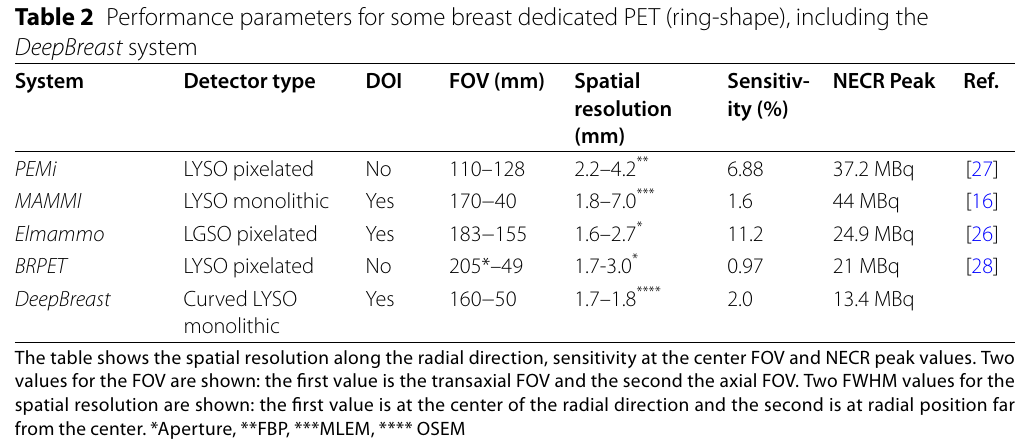
\includegraphics[width=0.9\linewidth]{img/freire2026-table2.png}
\end{center}

\paragraph{Why it matters here}
Three things. First, the reason the tube was not scaled: the authors say the
single-crystal approach of \ref{note:Freire2022} ``could not be applied'' at
\mm{200} bore ``because of limitations in the scintillation crystal growth
process of LYSO'', citing a 2013 J.\ Cryst.\ Growth paper. That is a stated
physical ceiling on the one-crystal annulus, and a reason any clinical-scale
annulus becomes segments optically joined. It also implies the rodent tube
was one grown piece. \gap{Confirm against \ref{note:Freire2022} and the cited
growth paper; what bore does LYSO growth allow?}
Second, it takes i3M's annular geometry past preclinical scale and couples it
to neural positioning (\ref{note:Freire2022a}), so the two detector lines
noted above have met in one scanner. Third, it names its own open items: no
TOF (they estimate about \ps{100} CTR would be needed to matter at this
bore), no randoms, dead-time or quantitative corrections, a short axial
length.

The gap they do not name is multiple interactions. Every event is reduced to
one point: the networks sum light across all 14 crystals and return a single
$(x,y)$, depth is one $E/I_{\max}$ ratio, and nothing detects, separates or
orders Compton scatter inside the ring. The glue makes this worse, not
better: light crossing the joints is the design, so a photon that scatters
from one crystal into the next lands in one merged light distribution that
the network was never trained to split (training used a fan beam, with low
centre-of-gravity events filtered out). That is the multi-vertex problem this
thesis takes up, on the one built scanner where the geometry most invites it.

\end{papernote}

\begin{papernote}{Cucarella et al.\ 2026 -- Development of a preclinical PET scanner with DOI capabilities using semi-monolithic detectors}{Cucarella2026}
\thumb{img/cucarella2026.png}
IEEE Trans.\ Radiat.\ Plasma Med.\ Sci.\ 10(7):1143--1151,
\doi{10.1109/TRPMS.2025.3648052}. Cucarella, Freire, González, Sánchez,
Gonzalez-Montoro, Jiménez-Serrano, Loignon-Houle, Moliner, Valladares,
Bruyndonckx, Correcher, Benlloch --- i3M with Bruker BioSpin. Open access.

\paragraph{Detector}
Two rings of 14 blocks, \mm{106} bore, \mm{52} axial, \mm{1.26} between the
rings. Each block is 22 LYSO slabs of \qtyproduct{0.97 x 25.6 x 12}{\mm}, the
long side axial, with a retroreflector on the entrance face, ESR between the
slabs and the narrow faces rough and black; glued to an 8 x 8 Hamamatsu array
at \mm{3.2} pitch, every one of the 1792 channels read by PETsys TOFPET2. Slab
from the centroid; position along the slab by one small network on the eight
summed signals, trained on a slit scan of a single module and used unchanged on
all 28; depth from $E/I_{\max}$, converted to mm by fitting its distribution in
flood data --- so only the network needs a collimated scan, and only once.

\paragraph{Key Findings}
\begin{itemize}
	\item Detector: \mm{1.7} FWHM along the slab, DOI \mm{3.08} at \mm{12}
		thick (side slit), slabs resolved with peak-to-valley 4.64; energy
		16.4\% (13.5\% centre) before a saturation correction they estimate
		would worsen it by about 30\%; CTR \ps{252} at detector level, but no
		system time-skew correction yet, so no TOF in the images.
	\item System, NEMA NU 4: \mm{1.61} mean at the centre (1.2/0.95/2.7
		radial/tangential/axial --- the gap between rings spoils the axial),
		\mm{1.0} at a quarter of the axial field; peak sensitivity 3.5\%
		(358--\keV{664}); NECR 106.9 kcps at \MBq{11.7}; CRC 0.20--0.85 for
		1--\mm{5} rods; \mm{1} Derenzo rods resolved.
	\item DOI correction improves radial resolution off centre, with residual
		degradation the authors put down to the DOI calibration.
	\item Table IV sets it against 17 preclinical scanners; it sits in the
		lower half (about 12th of 18 at \mm{1.61}); the authors call it
		``equivalent to other systems''.
\end{itemize}
\aside{The paper calls itself the first semi-monolithic preclinical scanner;
Aachen's 24-block one in \ref{note:Thull2026} contests that.}

\paragraph{Table IV against this map}
Of the monolithic entries, the map holds DigiPET (\ref{note:Espana2014}) and the
$\beta$-CUBE (\ref{note:Krishnamoorthy2018}) --- whose 12.4\% at
255--\keV{765} the table quotes as about 8\%, read off a plot for a narrower
window. Albira is \ref{note:Pajak2016} and the KU Leuven 7\,T insert
\ref{note:Gsell2020}. Of the pixelated ones, the DOI systems are the honest
comparators: QST's SR-PET (\ref{note:Kang2023}, three staggered layers) and
SIAT's dual-ended aPET (\ref{note:Kuang2020}). The rest are pixelated without
DOI and off this map's theme.

\paragraph{Why it matters here}
The measured semi-monolithic preclinical system whose full ring
\ref{note:Kuang2026a} only simulates (it measures a rotating two-detector
prototype), and a lower one: 3.5\% against 5.45\% simulated, \mm{1.6} against
about 1.1--\mm{1.4} without PSF modelling (sub-\mm{1} with it). Two things carry over. One network for every module is the
calibration economy a monolithic annulus needs. And the scanner is built as the
absorber of a Compton-PET with a thin scatter ring inside it
(\ref{note:Valladares2024}, on the plan of \ref{note:Ilisie2018}) --- i3M
taking the multi-interaction problem to two layers, where this thesis takes it
into one thick bulk.

\end{papernote}

\begin{papernote}{Pajak et al.\ 2016 -- NEMA NU4-2008 performance evaluation of Albira: a two-ring small-animal PET system using continuous LYSO crystals}{Pajak2016}
\thumb{img/pajak2016.png}
Open Med.\ J.\ 3:12--26, \doi{10.2174/1874220301603010012}. Pajak, Volgyes,
Pimlott, Salvador, Asensi, McKeown, Waldeck, Anderson --- Beatson Institute and
Glasgow, with Oncovision, i3M and Bruker. Open access (CC BY-NC).

\paragraph{Summary}
An independent NEMA evaluation of the first commercial monolithic PET. Two
octagonal rings of eight blocks, each one LYSO crystal shaped as a truncated
pyramid (\qtyproduct{50 x 50}{\mm} at the base, \qtyproduct{40 x 40}{\mm} at
the face, \mm{10} deep), on multi-anode PMTs with shared readout; \mm{111}
ring, \mm{94.4} axial. The tapering leaves a \mm{14.4} gap between the rings
at the front, right at the axial centre. Nothing is said about how position,
depth or energy are estimated beyond real-time continuous DOI, parallax
correction and a 300 x 300 virtual pixelation; it cites earlier papers.

\paragraph{Key Findings}
\begin{itemize}
	\item Resolution (MLEM, 30\% window): 1.72/1.70/\mm{2.45} radial/tangential/
		axial at the centre; 1.52/1.69/\mm{1.45} at a quarter of the axial field.
		Filtered back-projection cannot be done at the centre, in the gap.
	\item Peak sensitivity 5.3\% (255--\keV{767}), 4.2\% (358--\keV{664}).
	\item NECR 72 kcps at \MBq{7.1} (mouse), peaking early because the
		shared readout saturates; scatter fraction 9.8\%.
	\item Image quality: uniformity 4.9\%, RC 0.05--0.90 for 1--\mm{5} rods,
		spill-over 0.22 water, 0.14 air.
	\item The authors argue NEMA NU 4 penalises such geometries: the best
		resolution sits at the centre of each ring, not of the scanner.
\end{itemize}

\paragraph{Why it matters here}
The baseline a monolithic preclinical scanner started from in 2016: about
\mm{1.7} in plane, 5\% sensitivity, and a count rate set by the electronics,
not the crystal. No detector-level figure at all --- not DOI, not energy ---
so the monolith is only visible through its images.

\end{papernote}

\begin{papernote}{Gsell et al.\ 2020 -- Characterization of a preclinical PET insert in a 7 tesla MRI scanner: beyond NEMA testing}{Gsell2020}
\thumb{img/gsell2020.png}
Phys.\ Med.\ Biol.\ 65(24):245016, \doi{10.1088/1361-6560/aba08c}. Gsell,
Molinos, Correcher, Belderbos, Wouters, Junge, Heidenreich, Vande Velde,
Rezaei, Nuyts, Cawthorne, Cleeren, Nannan, Deroose, Himmelreich, González ---
KU Leuven with Bruker and i3M.

\paragraph{Summary}
The Bruker PET insert for a 7\,T MRI, the Albira line moved to SiPMs: three
rings of eight \qtyproduct{50 x 50 x 10}{\mm} monolithic LYSO blocks on 12 x 12
SiPM arrays at \mm{4.2} pitch, row-and-column readout; \mm{80} transaxial and
\mm{150} axial field. Mostly an MR-compatibility study, run under five MRI
sequences; positioning and DOI estimation are not described (refers to
González et al.\ 2016).

\paragraph{Key Findings}
\begin{itemize}
	\item Resolution (MLEM): 0.68/0.86/\mm{1.10} radial/tangential/axial at the
		centre and about \mm{0.92} on average out to \mm{35} off centre --- flat,
		which the authors credit to DOI.
	\item DOI about \mm{1.6} FWHM at \mm{10} thick, but fitted from flood data
		with no collimated beam; energy 16.6\% at low activity, 18.5\% at high,
		blamed on pile-up. No timing.
	\item Peak sensitivity 11.0\% (window not stated); NECR 486 kcps (mouse);
		\mm{0.7} Derenzo rods resolved; RC 0.14--0.95, uniformity 6.5\%.
	\item The MRI sequences change almost nothing: DOI worsens to 2.2 and
		\mm{2.1} (modules 0 and 10) only under FLASH.
\end{itemize}

\paragraph{Why it matters here}
What the monolithic preclinical line reached commercially: sub-millimetre and
flat to \mm{35} off centre, at 11\% sensitivity, against Albira's \mm{1.7} and
5\% four years before (\ref{note:Pajak2016}). Thin crystals and continuous DOI
do it; nothing about multiple interactions, and no TOF.

\end{papernote}

\begin{papernote}{Ilisie et al.\ 2018 -- Building blocks of a multi-layer PET with time sequence photon interaction discrimination and double Compton camera}{Ilisie2018}
\thumb{img/ilisie2018.png}
Nucl.\ Instrum.\ Methods A 895:74--83, \doi{10.1016/j.nima.2018.03.076}.
Ilisie, Giménez-Alventosa, Moliner, Sánchez, González, Rodríguez-Álvarez,
Benlloch --- i3M. Simulation (PENELOPE and GATE, agreeing within 1\%).

\paragraph{Summary}
The plan behind i3M's 4D-PET. A 511\,keV photon in LYSO is about as likely to
Compton scatter as to be absorbed (48.8 against 45.5\%; LaBr$_3$ 65.2 against
29.2\%), and a scattered event inside the photopeak is reduced to an
energy-weighted centroid. If every interaction and its order were known, the
first one gives the true line --- the thumbnail's top row against the centroid
images below. To use the scatter instead of averaging it: a ``double Compton
camera'', where the two photons' Compton cones must both contain the line, which
reduces to comparing the cosine of each geometric angle with the Compton angle
from the energies. That rejects randoms, patient scatter and wrong pairings in
multiple coincidences.

\paragraph{Key Findings}
\begin{itemize}
	\item Doppler broadening makes the Compton-angle error sharply non-Gaussian;
		treating it as Gaussian overstates it, so they propagate it by Monte
		Carlo.
	\item The stated premise: monolithic blocks on SiPMs \emph{cannot}
		separate several interactions well enough, so the design is
		multi-layer --- thin \mm{3}--5 LaBr$_3$ scatterers, a \mm{20} LYSO
		absorber, about \mm{30} apart so that \ps{100} TOF can order the hits.
	\item A \mm{3} LaBr$_3$ layer interacts with 21\% of photons; 41.5\% of
		those are one clean forward Compton, so 8.8\% of all photons (11.7\% at
		\mm{5}).
	\item The full matching algorithm and system simulation are deferred.
\end{itemize}

\paragraph{Why it matters here}
The clearest statement of the opposite bet to this thesis: separate the
interactions by building layers far apart and ordering them by time of flight,
because a single monolith cannot. \ref{note:Valladares2024} then measures
\ps{192} and finds the layers are too close for that. A thick bulk that
resolves its own interactions would make the layers unnecessary --- and this
paper's ideal-first-interaction Derenzo is the picture of what is at stake.

\end{papernote}

\begin{papernote}{Valladares et al.\ 2024 -- Detector characterization of a high-resolution ring for PET imaging of mice heads with sub-200-ps TOF}{Valladares2024}
\thumb{img/valladares2024.png}
IEEE Trans.\ Radiat.\ Plasma Med.\ Sci.\ 8(8):876--885,
\doi{10.1109/TRPMS.2024.3432194}. Valladares, Barrio, Cucarella, Freire, Vidal,
Benlloch, González --- i3M. Open access.

\paragraph{Summary}
The inner scatter layer of the 4D-PET: four flat detectors around a \mm{29}
square bore, eight modules of 24 x 24 Ca-codoped LYSO pixels
\qtyproduct{0.95 x 0.95 x 3}{\mm}, nine pixels to each \qtyproduct{3 x 3}{\mm}
SiPM with no light guide, every channel read by PETsys TOFPET2. The absorber
outside it is \ref{note:Cucarella2026}. Detector characterisation only: no
images, no DOI (\mm{3} thick), and no Compton events processed.

\paragraph{Key Findings}
\begin{itemize}
	\item CTR \ps{229} with skew correction, \ps{196} with time walk, \ps{192}
		with a within-SiPM transit-time correction; pixels 155--\ps{240}.
	\item Timing worsens at low energy: \ps{230} at 300--\keV{400}, \ps{286} at
		200--\keV{300}, over \ps{500} below \keV{200} --- the energies of the
		scattered deposits a Compton scheme needs.
	\item Energy 10.8\% after gain equalisation, 19.9\% after calibration to
		keV: nine pixels share one SiPM, which saturates.
	\item The authors' own conclusion: \ps{192} needs the layers about \mm{58}
		apart to tell which was hit first; they are \mm{38.5}. So TOF cannot
		order the interactions, and the ring is repurposed as a magnifying
		insert.
\end{itemize}

\paragraph{Why it matters here}
The measured answer to \ref{note:Ilisie2018}: even at a sub-\ps{200} CTR, time
of flight does not order two interactions centimetres apart. Ordering inside a
thick monolith, millimetres apart, cannot come from one timestamp per event; it
has to come from the photon arrival pattern --- which is the thesis.

\end{papernote}


 
\end{programnote}
 
 
% ===========================================================================
% 5. Aachen. Verified; Thull2026 nests inside as its paper.
% ===========================================================================
 
\begin{programnote}{RWTH Aachen -- Schulz group / Hyperion}{Aachen}
\location[150,-820]{50.78}{6.08}{Aachen, Germany}
 
\paragraph{What it is}
Two RWTH units, which matters for reading the author lists: the Department of
Physics of Molecular Imaging Systems (PMI, within Experimental Molecular
Imaging) and the Chair of Imaging and Computer Vision (LfB). Volkmar Schulz
holds posts in both, plus Hyperion Hybrid Imaging Systems GmbH and the
Fraunhofer Institute for Digital Medicine MEVIS, Bremen.
 
\aside{Thull's own address is LfB --- he came into PET from hematopoietic cell
classification, which is visible in the paper's shape: a computer-vision
treatment of a detector-physics problem.}
 
\paragraph{Platform}
Hyperion III preclinical PET/MRI; also the Hypmed scanner. Semi-monolithic LYSO
blocks with Philips DPC digital SiPMs. \textbf{Commercial arm} --- Hyperion is a
spin-off, not a paper affiliation of convenience.
 
\paragraph{Why it matters here}
They own light-distribution localisation uncertainty on real hardware, and they
have announced the follow-ups: multi-cluster event analysis, relating
light-spread structure to predicted uncertainty, and characterising inter-crystal
Compton scatter impact on positioning uncertainty. With a built scanner, a
fan-beam rig, four RTX 6000 Ada GPUs and a commercial arm, the
light-distribution version of ICS characterisation should be treated as theirs.
 
\paragraph{People}
Volkmar Schulz (chair), Julian Thull, Jan Remennik, David Schug, Björn Weissler,
Yannick Kuhl. Also Stefan Gundacker, Vanessa Nadig (TOF/DOI detector units,
TRPMS 2024)\aside{ --- relevant separately for the BGO and Cherenkov work}.
 
\paragraph{Adjacent outputs}
\begin{itemize}
	\item Kuhl, Mueller, Thull, Naunheim, Schug, Schulz --- 3D in-system
		calibration method for PET detectors, \emph{Medical Physics}.
		\gap{Year and volume. This is the ``calibration in hours not weeks''
		claim that closes ``calibrate faster'' as a contribution.}
	\item Kuhl, Thull, Gegenmantel, Weissler, Schug, Schulz --- In-system
		calibration demonstrated on Hypmed, 2025 IEEE NSS/MIC/RTSD, Yokohama.
	\item Thull, Remennik, Kuhl, Schulz --- ML-based uncertainty estimation for
		PET gamma interaction localisation, 2025 NSS/MIC. The conference
		precursor to \ref{note:Thull2026}.
	\item Thull, Mueller, Schulz --- Sinogram-based alignment estimation of PET
		detector blocks, 2024 NSS/MIC.
\end{itemize}
 
\begin{papernote}{Thull et al.\ 2026 -- Uncertainty-aware gamma interaction localisation and reconstruction}{Thull2026}
\thumb{img/thull2026.png}
Med.\ Phys.\ 53:e70471, \doi{10.1002/mp.70471}. Thull, Remennik, Schug, Weissler,
Kuhl, Schulz.

\paragraph{Summary}
Aachen (Schulz group, RWTH; three authors --- Schug, Weissler, Schulz --- also at Hyperion Hybrid Imaging Systems GmbH)
train localisation networks that emit a per-event positional variance alongside the
position estimate, then use that variance to filter and weight LORs during TOF-OSEM
reconstruction. Fully experimental: no simulation anywhere in the paper. The system is a
proof-of-concept preclinical scanner of 24 semi-monolithic LYSO blocks at \mm{62.5} inner
radius on the Hyperion III platform. Each block is
\qtyproduct{48.4 x 48.3 x 10}{\milli\metre} (planar-segmented,
planar-monolithic, DOI), built from two arrays of 44 polished LYSO slabs of
\qtyproduct{1 x 24 x 10}{\milli\metre} separated by \mm{0.1} BaSO$_4$, with a \mm{0.3}
light guide onto a 12 x 12
channel SiPM array formed from a 6 x 6 grid of Philips DPC3200-22 digital SiPMs.
Baseline detector performance is 12.7\% energy resolution and approximately \ps{500} CTR.

\paragraph{Capsule}
Thull et al.\ \cite{Thull2026} train per-detector, per-axis localisation networks on a
24-block semi-monolithic LYSO preclinical scanner that predict a positional variance
alongside each position estimate, then use that variance to filter and weight LORs in
TOF-OSEM reconstruction --- entirely on measured data. Headline result: the median
LOR-to-point-source distance falls from \mm{20.7} unfiltered to \mm{0.983} under combined
energy and variance filtering at 50\% retention (about 35\% effective), with variance the stronger and
complementary criterion because energy is a non-monotonic proxy for localisation quality
while predicted variance is monotonic. The work demonstrates rather than characterises:
$\sigma$ is rank-ordered but never calibrated, timing information is discarded, the
detector is fixed, and calibration cost is severe (weeks per scanner, 55 networks).
For this thesis it is the standing evidence that localisation confidence is a
first-class quantity, and it marks the light-distribution route as taken --- leaving the
temporal axis and information-theoretic bounds open.

\paragraph{Key Findings}
\begin{itemize}
    \item \textbf{Unfiltered localisation error dominates rather than dilutes.} Median
        distance from reconstructed LOR to a known point-source location is
        \textbf{\mm{20.7}} with no filtering. Energy windowing at 50\% retention brings this
        to \mm{2.4}; variance filtering at 50\% retention to \mm{1.12}; combined energy and
        variance filtering to \textbf{\mm{0.983}} (Table 4; the combined figure is
        about 35\% effective retention and a different model from the other two). This is the single most quotable number
        in the paper.
    \item \textbf{Variance outperforms energy as a filtering criterion, and the two are
        complementary.} Mean absolute error at 50\% singles retention (segmented /
        monolithic / DOI, in mm): energy filtering 0.49 / 0.72 / 1.03; variance filtering
        0.25 / 0.53 / 0.90; variance after energy 0.17 / 0.47 / 0.83 at about 35\%
        effective retention (0.243 / 0.527 / 0.892 at 49\%). Unfiltered CNN classifier is approximately \mm{1.1} in all three
        dimensions.
    \item \textbf{Energy is a non-monotonic proxy for localisation quality; predicted
        variance is monotonic.} MAE versus deposited energy shows a minimum at \keV{511}, a
        second minimum near \keV{340} (Compton backscatter, \degs{180}, producing a single
        light cluster), and elevated error between them --- a single Compton interaction
        cannot deposit intermediate energy, so that band is necessarily multi-scatter.
        Above \keV{511}, error rises again from pile-up and $^{176}$Lu background. MAE versus
        predicted $\sigma$ is monotonic with growing dispersion, i.e.\ a heavy-tailed error
        distribution.
    \item \textbf{A low-energy, low-variance population exists} (most visible in the
        monolithic and DOI dimensions) that energy windowing discards but variance
        filtering retains; the authors speculate these are geometrically well-constrained
        events occurring directly above a SiPM.
    \item \textbf{Image quality improves, at a noise cost.} With statistics restored to
        250 M coincidences, 50\% singles filtering gives PSNR 14.603 $\to$ 14.899,
        SSIM 0.405 $\to$ 0.462, COV 4.90\% $\to$ 4.66\%. Without restoring counts
        (62.5 M coincidences) COV degrades to 7.49\%. Peak-to-valley ratio on the \mm{0.8}
        rods rises from 1.0985 to 1.1840 under filtering and to 1.2171 under LOR weighting
        at $p = 4$, but COV at $p = 4$ blows out to 10.19\%. Filtering dominated weighting
        at matched effort; recovery coefficients improved at every rod diameter under both.
    \item \textbf{CNN classifiers beat regressors in-plane; CNN regressors win DOI.}
        Classifiers show systematically lower bias, and flood maps show regressors
        producing regions of near-zero prediction density where the continuous output
        collapses.
\end{itemize}

\paragraph{Methods Worth Noting}
\begin{itemize}
    \item \textbf{Heteroscedastic training.} Regressors train with a Gaussian
        negative log-likelihood,
        \[\mathrm{NLL} = \sum_n \bigl[\tfrac{1}{2}\log \sigma_n^2
            + (y_n - \hat{y}_n)^2 / 2\sigma_n^2\bigr],\]
        jointly predicting position and variance. Classifiers use ordinary
        cross-entropy over position bins, with uncertainty taken as the \emph{variance of
        the predicted softmax distribution} --- no special loss required.
    \item \textbf{Per-axis decomposition.} One independent network per detector per spatial
        dimension; 55 networks in total (7 central detectors x 3, 1 central x 2, 16 outer
        x 2). Optuna HPO over 12 configurations, approximately 377 trials each.
    \item \textbf{Fan-beam calibration.} Physical collimated fan of \mm{0.5} width on a
        motorised stage with \um{2} repeatability. Segmented axis: 44 positions at \mm{1.1}
        pitch, 20{,}000 samples each. Monolithic: 96 positions at \mm{0.5} pitch, 9{,}166
        each. DOI: 40 positions at \mm{0.25} pitch, 22{,}000 each. Roughly 880{,}000 events
        per detector per dimension, split 60/20/20. \textbf{Acquisition for the full
        scanner took several weeks.} DOI calibration fires \emph{parallel} to the
        photosensor face, so the lateral coordinate is deliberately unconstrained and
        marginalised over --- the per-axis decomposition is what makes this admissible.
        Only 7 of the 8 central-ring detectors could be labelled in all three dimensions; the 16
        outer detectors have monolithic and DOI labels only and borrow a segmented model.
    \item \textbf{Triggering is inherited, not designed.} The paper does not describe a
        trigger scheme; it uses the DPC die-level two-stage trigger and validation (Frach
        2009). The only stated acquisition-time selection is retention of readouts with
        more than 500 detected photons; no energy window is applied until evaluation.
    \item \textbf{Normalisation is recomputed under each filter and weight condition}
        (fan-sum method), which is what keeps the result quantitative rather than
        cosmetically sharper. Uncertainty is combined as
        $\sigma_{3D} = \sqrt{\sigma^2_{\mathrm{seg}} + \sigma^2_{\mathrm{mono}} +
        \sigma^2_{\mathrm{doi}}}$, and LOR weights as
        $w_{\mathrm{LOR}} = 1 / (\sigma_{3D,I_1} \cdot \sigma_{3D,I_2})^p$.
    \item \textbf{Reconstruction:} list-mode TOF-OSEM, 20 iterations, 10 subsets,
        \mm{0.2} isotropic voxels, 250 M coincidences,
        \qty[separate-uncertainty=true]{511 \pm 80}{\kilo\electronvolt} window,
        20 LORs sampled per coincidence. Phantoms: cylindrical shell (normalisation),
        HotRod with 2.0/1.5/1.2/1.0/0.9/\mm{0.8} rods at approximately \MBq{5} initial
        $^{18}$F-FDG, and a \MBq{1.5} $^{22}$Na point source at \mm{25} and \mm{35} radii.
    \item \textbf{Interpretation ceiling.} Label precision is \mm{0.5} (monolithic) and
        \mm{0.25} (DOI) with a \mm{0.5} fan width, so sub-\mm{0.5} MAE figures are not
        interpretable --- the authors say so, and introduce the LOR-to-point-source metric
        specifically to sidestep this.
\end{itemize}

\paragraph{Relevance to This Thesis}
This is the strongest published evidence for the premise that poorly localised
interactions actively damage reconstruction rather than weakly informing it, and it
forecloses the naive form of that idea: per-event uncertainty propagated into
reconstruction via filtering and weighting is done, on real hardware, with normalisation
handled correctly. Cite the \mm{20.7} unfiltered median LOR distance and the non-monotonic
energy--MAE curve as motivation; do not re-derive them.

What the paper does \emph{not} do:
\begin{itemize}
    \item \textbf{It demonstrates rather than characterises.} No Fisher information, no
        CRLB, no bound of any kind. One detector topology, one activity, an empirical
        threshold sweep. There is no crossover analysis for when rejecting a fraction $f$
        buys back more in bias than it costs at $1/\sqrt{1-f}$ in variance.
    \item \textbf{$\sigma$ is rank-ordered, never calibrated.} That $p = 4$ outperforms
        $p = 2$ is a direct tell: if $\sigma$ were a calibrated standard deviation,
        inverse-variance weighting would be optimal by construction. The authors do not
        remark on this. A rank-correct $\sigma$ does not transfer between detectors and
        does not compose across the two singles of a coincidence in any principled way.
    \item \textbf{Timing is entirely unused.} Network inputs are the 144 SiPM photon counts
        and nothing else. The 36 dies supply up to 36 independent timestamps per event at
        approximately \ps{500} CTR, all discarded, along with the pattern of \emph{which}
        dies triggered. The authors state that Compton interaction \emph{sequence} cannot
        be inferred from the light pattern because scintillation emission is isotropic ---
        true of photon counts, but not of arrival times.
    \item \textbf{The detector is fixed.} No design feedback; $\sigma$ is a measurement
        outcome, never an objective.
    \item \textbf{Aleatoric and epistemic uncertainty are not disentangled}, which the
        authors acknowledge: a deterministic network emitting a variance is nominally
        claiming aleatoric uncertainty but is contaminated by finite training data and
        model capacity.
\end{itemize}

\paragraph{Where It Might Go}
Motivation for any chapter arguing that localisation confidence is a first-class quantity;
the \mm{20.7} figure belongs in an introduction. Also the reference point for calibration
burden (several weeks per scanner, 55 networks, outer-ring detectors physically
unlabellable in the segmented direction) --- though note the group's own in-system
calibration work (Kuhl et al.\ 2025) claims to reduce this to hours via virtual
collimation, so ``calibrate faster'' is taken and ``design so that calibration is cheap''
is not.

\emph{Competitive note:} the discussion explicitly announces future work analysing
multi-cluster events, relating light-spread structure to predicted uncertainty, and
characterising the impact of inter-crystal Compton scatter on positioning uncertainty.
Aachen has the built scanner, the fan-beam rig, four RTX 6000 Ada GPUs and a commercial
arm. The light-distribution version of ICS characterisation should be treated as theirs.
The temporal axis --- cardinality and interaction ordering inferred from the joint
distribution of per-channel arrival times rather than from photon counts --- and the
information-theoretic bound on separability are the surviving directions. Note that
Carra et al.\ 2022 runs information both ways --- its joint layer uses timing to
refine position as well as light to refine timing (\ref{note:Carra2022}) --- and
J-PET positions along a strip from timing (\ref{prog:J-PET}), so ``time informs
position'' is not new; what is unaddressed is cardinality and ordering from
per-channel arrival times.
\end{papernote}
 
\end{programnote}
 
 
% ===========================================================================
% 6. NEW -- Ghent, disentangled from UTOFPET. Partially verified.

% ===========================================================================
% 6. Ghent MEDISIP -- the detector thread. The system thread is 6a. Partially
% verified.
% ===========================================================================

\begin{programnote}{Ghent MEDISIP -- the monolithic detector lineage}{Ghent}
\location[-960,200]{51.05}{3.72}{Ghent, Belgium}

\paragraph{Why separate from UTOFPET}
Ghent has a monolithic lineage that predates and runs parallel to the
consortium. Nesting Stockhoff 2021 and Decuyper 2021 under \ref{prog:UTOFPET}
implies more coordination than the evidence supports. Keep the nodes distinct
and cross-reference; UTOFPET is the joint detector project, not the whole of
either group.

\paragraph{Why separate from WT-PET}
This node was nine papers doing two jobs. The detectors and the positioning
stay here; the total-body system designs built on them are \ref{prog:WTPET},
and the spin-off that sells one is \ref{prog:Molecubes}. Three nodes, one pin
--- Ghent is the single most productive address on this map, and the threads
make different claims.

\paragraph{What it is}
Medical Image and Signal Processing (MEDISIP), Department of Electronics and
Information Systems, Ghent University. PI Stefaan Vandenberghe. The thread
here is the detector itself: thin monolithic crystals in
\ref{note:Espana2014}, a characterised \qtyproduct{50 x 50 x 16}{\mm} block
in \ref{note:Stockhoff2021}, and a positioning network for it in
\ref{note:Decuyper2021}.

\paragraph{People}
Vandenberghe (PI), Roel Van Holen, Mariele Stockhoff, Milan Decuyper, with
Jens Maebe on the positioning-and-timing work.

\paragraph{Key outputs}
\begin{itemize}
	\item Espa\~na et al.\ 2014 PMB --- DigiPET, the start of the lineage
		(\ref{note:Espana2014}).
	\item Stockhoff et al.\ 2021 PMB --- the measured block
		(\ref{note:Stockhoff2021}), \qtyproduct{50 x 50 x 16}{\mm}: the one the
		walk-through panels are built from, not the \qtyproduct{25.4 x 25.4 x 8}{\mm}
		block \ref{prog:Molecubes} ships.
	\item Decuyper et al.\ 2021 PMB --- the positioning network
		(\ref{note:Decuyper2021}). Kill (g).
	\item Maebe \& Vandenberghe 2022, ``Simulation study on 3D convolutional
		neural networks for time-of-flight prediction in monolithic PET
		detectors using digitized waveforms'', PMB 67(12):125016 --- TOF
		prediction, not joint position and timestamp.
\end{itemize}

\paragraph{Why it matters here}
Much of what \ref{prog:WTPET} claims at system level rests on this node: a
real monolith at \mm{1.14} intrinsic over its whole face, with a network that
slightly beats nearest neighbour on it, both measured
(\ref{note:Stockhoff2021}, 1.14 against \mm{1.17}); and a simulated ceiling for
network positioning (\ref{note:Decuyper2021}). If a thesis wants to contest the panel campaign, this is
where the contestable number actually lives --- not in the system simulations,
which only inherit it.

\paragraph{Thesis entry}
The review folds this node and \ref{prog:UTOFPET} into one programme entry,
``UTOFPET: Pisa and Ghent, from DigiPET to walk-through PET'', because the
WT-PET paper itself names UTOFPET as the detector's origin. Pisa is credited
for the positioning-and-timing network (\ref{note:Carra2022}), Ghent for DigiPET
and the WT-PET system. The separation kept here is for prior-art bookkeeping,
not something the thesis argues.

\begin{papernote}{Espa\~na et al.\ 2014 -- DigiPET: sub-millimeter spatial resolution small-animal PET imaging using thin monolithic scintillators}{Espana2014}
\thumb{img/espana2014.png}
Phys.\ Med.\ Biol.\ 59(13):3405, \doi{10.1088/0031-9155/59/13/3405}. Espa\~na,
Marcinkowski, Keereman, Vandenberghe, Van Holen.

\paragraph{Summary}
Sub-millimetre small-animal PET from thin monolithic LYSO slabs on digital
SiPMs: the thin slab trades stopping power for a light distribution narrow
enough to localise below a millimetre without DOI. The first monolithic
scanner in the Ghent line. Four \qtyproduct{32 x 32 x 2}{\mm} LYSO detectors
in a square, \mm{34.5} between opposite ones, each on a dSiPM module (the
figure's \mm{13} and \mm{38.5} label the module, not the crystal), with a fan
each. Positioning is maximum likelihood. Intrinsic resolution \mm{0.54} FWHM,
\mm{0.7} at the centre of the field; sensitivity 0.3\% (400--\keV{600}) or
0.6\% (250--\keV{650}); CRT \ps{680}; energy 18\%; ``no relevant DOI
effect'' in \mm{2}. The thin slab is argued on cost: thin unpixelated crystals
are cheap, and fine pixels make systems expensive.

\end{papernote}

\begin{papernote}{Stockhoff et al.\ 2021 -- High-resolution monolithic LYSO detector with 6-layer depth-of-interaction for clinical PET}{Stockhoff2021}
\thumb{img/stockhoff2021.png}
Phys.\ Med.\ Biol.\ 66:155014, \doi{10.1088/1361-6560/ac1459}. Stockhoff,
Decuyper, Van Holen, Vandenberghe.

\paragraph{Detector}
A \qtyproduct{50 x 50 x 16}{\mm} LYSO monolith (Epic Crystal), sides rough and
black-painted, top polished under a black-painted specular reflector, on an
8 x 8 array of \qtyproduct{6 x 6}{\mm} onsemi MicroFJ-60035 SiPMs at \mm{6}
pitch; a resistor network sums rows and columns, 64 pixels to 16 channels,
digitised free-running at 64 MHz. Measured, not simulated: a collimated
$^{68}$Ge beam of 0.6 or \mm{1.0}, 49 x 49 positions, with a 10 x 10 grid
offset by \mm{0.5} for validation.

\paragraph{Method}
Mean nearest neighbour (MNN) against a shallow network (three hidden layers of
256). The six ``virtual DOI layers'' are not measured depths: each event's
light is normalised, events at a position are sorted by the variance across
the 16 channels, and cut into six quantiles sized to Beer--Lambert
attenuation (29.5 / 23.0 / 17.9 / 13.9 / 10.8 / 4.9\% for MNN). DOI is
checked only as the share of events landing in each layer --- no side
irradiation, no DOI FWHM; the authors reject side irradiation because events
pile up at the edge. No Compton rejection beyond a 20\% energy window; about
60\% of events scatter.

\paragraph{Key Findings}
Intrinsic resolution \mm{1.14} FWHM over the whole face with a neural
network and \mm{1.17} with mean nearest neighbour; \mm{1.02} and \mm{1.13}
respectively over the central \qtyproduct{30 x 30}{\mm}. The stated target is
the \mm{1.3} intrinsic needed for \mm{2} at system level in whole-body PET.
2D bias falls from \mm{0.59} (MNN) to \mm{0.20} (network) over the face.
Energy resolution 11.0\% (10.7\% centre, up to 18\% in corners); no timing
reported. Bar phantom resolves 0.6--\mm{1.2} slits with both algorithms.
The network's gain is a centre gain: 9.7\% better FWHM in the central
\qtyproduct{30 x 30}{\mm} but 2.6\% over the whole face, so near the edges
it is roughly nil on FWHM, though its bias advantage survives. The paper's
own figures disagree in places (1.13 against 1.14, a ``1.5'' that Table 2 gives
as 1.15).

\paragraph{Why it matters here}
This is the block the walk-through work scales up from
(\ref{note:Vandenberghe2023}, \ref{note:AbiAkl2025}) and the same one
\ref{note:Decuyper2021} positions in simulation --- so the lineage's
detector, measured. Note the size: \qtyproduct{50 x 50 x 16}{\mm} here
against the \qtyproduct{25.4 x 25.4 x 8}{\mm} block
\ref{prog:Molecubes} sells. That smaller block is the one the WT-PET paper
means by its ``existing preclinical monolithic detectors [18]'' (the
$\beta$-CUBE, \ref{note:Krishnamoorthy2018}), scaled up by two to this size.

\end{papernote}

\begin{papernote}{Decuyper et al.\ 2021 -- Artificial neural networks for positioning of gamma interactions in monolithic PET detectors}{Decuyper2021}
\thumb{img/decuyper2021.png}
Phys.\ Med.\ Biol.\ 66:075001, \doi{10.1088/1361-6560/abebfc}. Decuyper,
Stockhoff, Vandenberghe, Van Holen.

\paragraph{Method}
A network of three hidden layers of 256 neurons maps the light distribution to
the first interaction position --- Compton or photoelectric --- in a
\qtyproduct{50 x 50 x 16}{\mm} LYSO monolith read out by a photodetector
array, trained on optical simulation where that first position is known.
\textbf{Simulation only:} GATE 8.0 with the measured-surface \texttt{LUT
Davis} model (\ref{note:Roncali2013}), an 8 x 8 array of \mm{6.07} SiPMs
at an idealised 75\% PDE, the 16 row and column sums as input. Training on a
49 x 49 grid at \mm{1} steps, 1000 events per position, L1 loss, with a
second grid offset by \mm{0.5} to catch the network snapping to training
positions --- which the larger networks do.

\paragraph{Key Findings}
Median 3D positioning error \mm{0.77} and 2D FWHM \mm{0.46}, a
\qty{17}{\percent} improvement in FWHM on nearest neighbour at the detector
centre with the same 16-channel readout (11\% over the whole detector, against
a 32-channel network); restricted to
non-Compton events, \mm{0.40} and \mm{0.42}. Continuous DOI comes from one
more output neuron, about 46\% better than nearest neighbour's six layers;
inference runs at 21 million events per second on one RTX 2080 Ti.

\textbf{Compton scatter.} About 60\% of
events scatter in the crystal before absorption, and for them the median 3D
error rises from \mm{0.40} to \mm{1.59} (means \mm{0.49} and \mm{2.29}),
the DOI error FWHM from \mm{0.71} to \mm{1.80}, and the position spread
grows long tails: 93\% more error overall than unscattered events alone. The
error has a direction --- most scatter is small-angle and forward, so the
light comes from nearer the sensor and the network places the event too
deep. The authors' remedy is in the discussion and not done: train networks to
recognise scattered events and position them separately.

No measured data: the authors say testing on real data is future work, and
that their DOI training has no counterpart in the lab, where the true depth of
the first interaction is unknown.\aside{ This note previously had it
transferring from simulation to measurement; it does not.}

\paragraph{Why it matters here}
Kill (g): the strongest published claim that a network beats nearest
neighbour on a monolith, and the one an annulus positioning argument has to
better or explain. Its ceiling is the first-interaction position, which only
simulation knows, and the paper never leaves simulation, so its \mm{0.46} is
a ceiling at an idealised PDE, not a measurement to set against a real
detector such as \ref{note:Stockhoff2021}.

It is also the cleanest published number for the multi-interaction problem in
a monolith: the majority of events, 60\% in \mm{16} of LYSO, are
multi-site, they carry most of the positioning error, and that error is
biased in depth. The authors name the next step --- detect the scattered
events, then treat them separately --- and stop there. The detecting half has
since been done, by \ref{note:Shen2025}: a classifier for one, two or
three-plus deposits, from photon counts, in simulated nanocomposite and
ceramic slabs. Treating them separately, locating more than the first
vertex, ordering them, and doing any of it from arrival times all remain
open.
\gap{Check whether Ghent later built the scatter-aware networks the
discussion proposes.}

\end{papernote}

\end{programnote}


% ===========================================================================
% 6a. WT-PET -- the system thread split out of Ghent. Four re-costings of one
% geometry; read them as one campaign, not six papers.
% ===========================================================================

\begin{programnote}{WT-PET -- Ghent's flat-panel total-body campaign}{WTPET}
\location[-1008,-896]{51.05}{3.72}{Ghent, Belgium}
\thumb{img/wtpet.png}

\paragraph{What it is}
The system-design thread of \ref{prog:Ghent}, under the same PI: stand the
patient upright between two flat panels of monolithic detectors instead of
lying them inside a cylinder, and buy resolution and sensitivity with
proximity rather than with crystal. Walk-through PET site:
\url{https://www.wt-pet.org/}. The detector is not its own --- it is the
\qtyproduct{50 x 50 x 16}{\mm} block of \ref{note:Stockhoff2021}, but its
assumed performance varies by paper: \ref{note:Vandenberghe2023} takes \ps{600}
for BGO and \ps{300} for LYSO; \ref{note:Dadgar2023} uses \mm{1.3} 2D, \mm{2}
DOI and \ps{327} cited from Carra 2022; \ref{note:AbiAkl2023} models \ps{200}
with Stockhoff's blurring; only \ref{note:AbiAkl2025} and
\ref{note:Dhaenens2026} use \mm{1.14}, \mm{2.67} and \ps{300}.
\gap{Funding and project status. The site reads like a funded project with a
named grant; find it, because ``a funded programme'' and ``a series of
simulation papers'' are different claims and this node currently asserts
neither.}

\paragraph{People}
Vandenberghe (PI), Jens Maebe, Maya Abi Akl, Meysam Dadgar, Boris Vervenne,
Elke Dhaenens, Florence Muller, Christian Vanhove.

\paragraph{Key outputs}
Six papers, and they are one argument rather than six results:
\begin{itemize}
	\item \ref{note:Vandenberghe2020} --- the cost-efficient total-body target the
		rest inherits, and the group's own case against monolithic readout cost.
	\item \ref{note:Vandenberghe2023} --- the walk-through design itself.
	\item \ref{note:Dadgar2023} --- panels against a cylinder, in BGO.
	\item \ref{note:AbiAkl2023} --- the same block wrapped into a ring instead.
	\item \ref{note:AbiAkl2025} --- panels thinned, gaps closed by moving them
		vertically.
	\item \ref{note:Dhaenens2026} --- panels narrowed, swept laterally.
	\item Maebe PhD thesis, Ghent 2024 --- ``Timing capabilities and image
		reconstruction for the walk-through PET''.
		\gap{Unread. The reconstruction half is where the limited-angle
		artefacts are either solved or conceded.}
\end{itemize}

\paragraph{Why it matters here}
Read in order, the campaign states its own weakness four times. Every
costing-down buys detectors back with angular coverage, and every paper ends
asking for better timing: \ref{note:Dadgar2023} weighs the panels against a
closed geometry, \ref{note:AbiAkl2025} reports
\qtyrange{3}{3.5}{\mm} perpendicular to the panel face, and
\ref{note:Dhaenens2026} concedes elongation artefacts in both its flat-panel
builds and asks for better than \ps{300} to suppress them. That is the
argument for a closed geometry made by the open-geometry camp itself --- an
annulus has no limited-angle artefact to buy off and no moving part to
schedule. It is also the reason \ref{note:AbiAkl2023} exists: when the same
group wrapped the same block into a ring, the comparison stopped being
rhetorical.

\paragraph{Scope boundary}
This node is system geometry. Detector physics, including the \mm{1.14} the
later papers assume, is \ref{prog:Ghent}; the productised preclinical
scanner is \ref{prog:Molecubes}.

\begin{papernote}{Vandenberghe et al.\ 2020 -- State of the art in total body PET}{Vandenberghe2020}
\thumb{img/vandenberghe2020.png}
EJNMMI Phys.\ 7:35, \doi{10.1186/s40658-020-00290-2}. Vandenberghe, Moskal, Karp.
Review, open access.

\paragraph{Summary}
The group's own survey of long-axial-field PET, and the citable home of their
PET20.0 design, which otherwise exists only as conference abstracts (EANM 2017;
Austrian Winter Symposium 2018): a compact total-body scanner with ``only 3--4
times the detector material of a current PET-CT'', using high-resolution
monolithic detectors to take ``a large step in spatial resolution'' as well as
sensitivity. Around it: sensitivity gains of 2.5--3.5x for a single organ
(saturating at \qty{70}{\centi\metre}) against up to 40x for a \qty{2}{\metre}
object; component cost dominated by crystal volume, photodetector area and
electronics.

\paragraph{On monolithic detectors}
\begin{itemize}
	\item Monolithic blocks cost about the same as pixelated ones at clinical
		pixel sizes (2--\mm{4}); the readout and positioning are what is ``more
		complex and costly'', and they call that ``a major limitation'' for
		total-body systems --- hoping faster FPGAs fix it.
	\item Timing is the hardest parameter, because the light spreads over more
		photodetectors; fast, accurate TOF estimators still have to be
		developed.
	\item Very good detector results in the lab, ``not yet \ldots realised in
		full systems''.
\end{itemize}

\paragraph{Why it matters here}
The cost and timing objections to a clinical monolith, stated by the group
most committed to building one: not the crystal but the readout and the
positioning, and not resolution but time. Those are the two things a thick
monolith with learned positioning has to answer. The walk-through panels
(\ref{note:Vandenberghe2023}) are their answer to the cost.

\end{papernote}

\begin{papernote}{Vandenberghe et al.\ 2023 -- Walk-through flat panel total-body PET: a patient-centered design for high throughput imaging at lower cost using DOI-capable high-resolution monolithic detectors}{Vandenberghe2023}
\thumb{img/vandenberghe2023.png}
Eur.\ J.\ Nucl.\ Med.\ Mol.\ Imaging 50(12):3558--3571,
\doi{10.1007/s00259-023-06341-x}.

\paragraph{Summary}
Two flat panels, each \qtyproduct{70 x 106}{\centi\metre}, \cm{50} apart,
the patient standing upright between them; 14 x 20 = 280 monolithic blocks
per panel, \qtyproduct{50 x 50 x 16}{\milli\metre} BGO or LYSO on 8 x 8
arrays of \qtyproduct{6 x 6}{\milli\metre} SiPMs with 6-layer DOI. Detector
surface is reduced 1.9x and scintillator volume 2.2x against a long-axial-FOV
cylinder at comparable sensitivity. \aside{System detail is held in
\ref{prog:UTOFPET}, including the block sizing by doubling.}

\paragraph{Why it matters here}
The clearest published statement that panel geometry is a \emph{cost}
argument rather than a performance one, and the paper that names UTOFPET as
the detector's origin.

\end{papernote}

\begin{papernote}{Dadgar et al.\ 2023 -- A simulation study of the system characteristics for a long axial FOV PET design based on monolithic BGO flat panels compared with a pixelated LSO cylindrical design}{Dadgar2023}
\thumb{img/dadgar2023.png}
EJNMMI Phys.\ 10:75, \doi{10.1186/s40658-023-00593-0}. Dadgar, Maebe, Abi Akl,
Vervenne, Vandenberghe.

\paragraph{Summary}
GATE comparison of the walk-through flat-panel BGO design against a pixelated
LSO cylinder: spatial resolution, sensitivity, count rate, scatter fraction
and image quality. The DOI-capable monolithic panels hold resolution below
\mm{2} in the directions parallel to the panels but reach \mm{3.36}
perpendicular to them; peak sensitivity \qty{154}{cps\per\kilo\becquerel},
against a cylinder that is coarser in resolution, more sensitive only with
no ring-difference cut (179.7 against 154 at MRD 322; 87.0 at MRD 85), and free
of the positioning constraint. The \mm{3.36} is the worst case, a point near a
panel at 3/8 of the axial field; the authors put it down to limited projection
angles. DOI is modelled as continuous Gaussian smearing (about \mm{2} FWHM),
not layers.

\paragraph{Why it matters here}
The honest self-assessment of the panel trade, from the group that proposed
it. Note the authorship: Dadgar and Maebe are joint first, Vervenne is fourth --- the reading
list had this as ``Vervenne \& Vandenberghe''.

\end{papernote}

\begin{papernote}{Abi-Akl et al.\ 2023 -- Monte Carlo simulation of the system performance of a long axial field-of-view PET based on monolithic LYSO detectors}{AbiAkl2023}
\thumb{img/abiakl2023.png}
EJNMMI Phys.\ 10:37, \doi{10.1186/s40658-023-00559-2}. Abi-Akl, Dadgar,
Toufique, Bouhali, Vandenberghe. Ghent MEDISIP with Texas A\&M University at
Qatar.

\paragraph{Summary}
GATE study of monolithic LYSO blocks, \qtyproduct{50 x 50 x 16}{\mm},
DOI-capable, 40 modules to a ring around a \cm{70} bore, in two lengths:
\cm{36.2} axial FOV over 7 rings and \cm{72.6} over 14. Sub-\mm{2} FWHM in
all three directions, central sensitivity \qty{29.2}{\kilo cps\per\mega\becquerel}
and \qty{106.8}{\kilo cps\per\mega\becquerel}, NECR peaks \qty{716}{\kilo cps}
and \qty{1235}{\kilo cps}, scatter fraction 32\%, timing modelled at \ps{200}.
\gap{Unread beyond the abstract and the numbers above. Read for how the DOI
layers are modelled and what the \ps{200} assumes, since the same block
appears in the walk-through work at a different granularity.}

\paragraph{Why it matters here}
The cylindrical counterpart to \ref{note:Dadgar2023}, from the same group
and the same simulation campaign: monolithic LYSO wrapped into a ring rather
than flattened into panels. Not a walk-through paper. It is the cleanest
published statement of what monolithic blocks with DOI reach in a conventional
cylinder --- sub-\mm{2} in every direction, where the panels lose to
\mm{3.36} perpendicular --- which makes it the comparison an annular
monolith such as \ref{prog:AnnPET} or \ref{prog:HUST} is measured against.
\aside{Abi Akl was already in the Ghent people list; this is the paper she
leads.}

\end{papernote}

\begin{papernote}{Abi-Akl et al.\ 2025 -- Performance evaluation of a medium axial field-of-view sparse PET system based on flat panels of monolithic LYSO detectors: a simulation study}{AbiAkl2025}
\thumb{img/abiakl2025.png}
EJNMMI Phys.\ 12:49, \doi{10.1186/s40658-025-00766-z}. Abi-Akl, Maebe,
Vervenne, Bouhali, Vanhove, Vandenberghe.

\paragraph{Summary}
The walk-through geometry costed down. Two vertical panels \cm{50} apart, in
two builds: the long panel at \cm{106} axial FOV over 20 detector rows, and a
sparse medium panel at \cm{60} over 8 rows with \mm{28} axial gaps --- about
half a detector width, closed by moving the panels vertically rather than by
buying detectors. Monolithic LYSO \qtyproduct{50 x 50 x 16}{\mm} with DOI,
intrinsic resolution \mm{1.14} parallel to the panel face and \mm{2.67} in
depth, CTR \ps{300}. The sparse build averages
\qty{26}{\kilo cps\per\mega\becquerel}, \num{4.6} times less sensitive than
the long one, holds sub-\mm{2} in the panel-parallel directions and
\qtyrange{3}{3.5}{\mm} perpendicular, and needs \qtyrange{2}{3}{\minute} to
match what the long panel does in \qty{30}{\second}.
\gap{Unread beyond the abstract. Read for how the panel motion is scheduled
and whether the gap is filled exactly or sampled, and for what the \ps{300}
rests on.}

\paragraph{Why it matters here}
The third point of the same campaign, and the one that prices the geometry:
\ref{note:Vandenberghe2023} proposed the panels, \ref{note:Dadgar2023} weighed
them against a cylinder in BGO, \ref{note:AbiAkl2023} wrapped the same
monolithic LYSO block into a ring, and this halves the detector count and
reports what that costs. The perpendicular \qtyrange{3}{3.5}{\mm} is the
panel geometry's standing weakness, in LYSO as in BGO --- the direction a
monolithic annulus does not have.

\end{papernote}

\begin{papernote}{Dhaenens, Vervenne et al.\ 2026 -- Simulation study of a low-cost Slide-Through PET scanner based on narrow flat panels with monolithic detectors}{Dhaenens2026}
\thumb{img/dhaenens2026.png}
Front.\ Phys.\ 13:1712273, \doi{10.3389/fphy.2025.1712273}. Dhaenens and
Vervenne (joint first), Abi Akl, Maebe, Vanhove, Vandenberghe. Ghent MEDISIP.

\paragraph{Summary}
The walk-through panels narrowed and put on rails. Two vertical panels
\cm{50} apart, each \cm{190.5} tall and stepped in width: \cm{20.9} across the
top for the torso, \cm{10.3} across the bottom for the legs. Instead of a panel
wide enough for the patient, the pair translates sideways to sweep a
\cm{73.9} field of view, 224 detector modules in all. The detector is the
lineage's own --- \qtyproduct{50 x 50 x 16}{\mm} monolithic LYSO on an 8 x 8
array of \qtyproduct{6 x 6}{\mm} SiPMs, with resolution values taken from
\ref{note:Stockhoff2021}, \ps{300} CTR and \mm{2.67} DOI.

\paragraph{Method}
GATE v9.4, against two references built from the same detectors: a wide static
flat panel and a cylinder. Three panel motions were tried (parallel, opposite,
single-panel), scored on NEMA image quality and XCAT phantoms.

\paragraph{Key Findings}
Only parallel motion covers the anatomy; the other two sample a focused region
and miss the rest. Sensitivity on a whole-body water phantom is
\qty{1.66}{cps\per\kilo\becquerel} in the upper section and
\qty{0.52}{cps\per\kilo\becquerel} in the lower, against
\qty{1.05}{cps\per\kilo\becquerel} everywhere for the cylinder --- so the
torso gains about half again and the legs lose half. Sub-\mm{3} at the centre
of the field of view. On torso noise, \mins{4} of ST-PET matches \mins{9.15}
of the cylinder. Both flat-panel systems show mild elongation artefacts from
the limited angular coverage, and the conclusion asks for better than \ps{300}
to suppress them.
\aside{This paper's sensitivity is a whole-body water phantom with
attenuation, while \ref{note:AbiAkl2025} quotes
\qty{26}{\kilo cps\per\mega\becquerel} on its own figure of merit. The units
are interconvertible and the numbers are not; do not put them in one table.}
Detector count is argued, cost is not: 224 detectors against 225 for a
standard cylinder, 1008 for the reference flat panels and 560 for the
original walk-through design, for \cm{190} of coverage; the conclusion claims
only a ``slightly reduced component cost''.
\gap{Worth reading for what the legs' \qty{0.52}{cps\per\kilo\becquerel}
means clinically, and how the lateral sweep is scheduled against tracer
kinetics.}

\paragraph{Why it matters here}
The fourth costing-down of one geometry, and the clearest statement of what
the panels keep paying with. \ref{note:Vandenberghe2023} proposed them,
\ref{note:Dadgar2023} weighed them against a cylinder in BGO,
\ref{note:AbiAkl2025} thinned them and closed the gaps by moving them
vertically, and this one narrows them and moves them sideways. Every step buys
detectors back with angular coverage, and every step ends asking for better
timing --- limited-angle elongation is the structural cost of a flat panel, and
\ps{300} is not enough to hide it. That is the argument for a closed geometry
stated by the panel camp itself: a monolithic annulus has no limited-angle
problem to buy off, and no moving part to schedule.

\end{papernote}

\end{programnote}
 
 
% ===========================================================================
% 6b. NEW -- Molecubes. The commercial arm of the Ghent lineage.
% ===========================================================================
 
\begin{programnote}{Molecubes -- Ghent spin-off, monolithic PET sold as a product}{Molecubes}
\location[-975,-379]{51.05}{3.72}{Ghent, Belgium}
\thumb{img/molecubes.png}
 
\paragraph{What it is}
A Ghent University spin-off selling benchtop preclinical scanners as a family
of stacking cubes: the $\beta$-CUBE (PET), $\gamma$-CUBE (SPECT) and X-CUBE
(CT). \url{https://www.molecubes.com/}. The $\beta$-CUBE is the monolithic
lineage of \ref{prog:Ghent} turned into a product --- monolithic LYSO with
DOI, maximum-likelihood clustering positioning, sold rather than demonstrated. Acquired by
Bruker on 19 November 2021 and run inside its BioSpin preclinical imaging
division; over 70 systems installed by then, on about 5 million euro of
2020 revenue.
\gap{Founding year: Qbic says 2015, another account 2016. Whether the
positioning network in the shipped product is the published one, and whether
anything of the calibration is documented outside the papers.}
 
\paragraph{People}
Roel Van Holen (co-founder, CEO), Pieter Mollet, Ewout Vansteenkiste, with
Stefaan Vandenberghe on the $\beta$-CUBE work --- the same people as
\ref{prog:Ghent}, which is why this is a separate node rather than a paper
inside it.
 
\paragraph{Literature}
Thin, and that is the point: one peer-reviewed performance paper
(\ref{note:Krishnamoorthy2018}), its IEEE NSS/MIC 2017 conference version and the makers' own JNM
abstract (\ref{note:Mollet2017}), then nothing until other groups' application papers that use a
$\beta$-CUBE as a platform rather than study it. No independent NEMA NU4
evaluation by a second lab, and no published account of the calibration a
shipped monolithic scanner needs.
\gap{Searched, not found --- worth one more pass before the thesis says
``none''. If it holds, the absence is itself evidence: the hard part of
monolithic PET is exactly what a vendor does not publish.}

\paragraph{Why it matters here}
The existence proof that a monolithic scanner can be productised: whatever a
thesis argues about calibration burden or positioning fragility has to survive
the fact that someone sells one and 70-odd labs run it. It also puts a
commercial floor under the annulus comparison --- \ref{prog:AnnPET} and
\ref{prog:HUST} are measured against \mm{1} at \qty{12.4}{\percent}, not
against a research prototype.
 
\begin{papernote}{Mollet et al.\ 2017 -- The beta-CUBE, a high-end compact preclinical benchtop PET for total body imaging}{Mollet2017}
\thumb{img/mollet2017.png}
J.\ Nucl.\ Med.\ 58(supplement 1):393,
\href{https://jnm.snmjournals.org/content/58/supplement_1/393}{jnm.snmjournals.org}.
Mollet, Deprez, Vandeghinste, Neyt,
Marcinkowski, Vandenberghe, Van Holen. A meeting abstract, not a paper: cite
it as one, and prefer \ref{note:Krishnamoorthy2018} wherever both cover the same
ground.

\paragraph{Detector}
The makers' own description of the shipped machine, which
\ref{note:Krishnamoorthy2018} does not give: nine modules to a ring, \mm{76} inner
diameter, \cm{13.3} axial FOV; five \qtyproduct{25.4 x 25.4 x 8}{\mm}
monolithic LYSO blocks per module on analogue Hamamatsu MPPCs, Peltier-held at
\qty{23}{\celsius}, per-pixel readout into five coincidence boards. Event
positioning is statistical and runs on a GPU in the acquisition server;
reconstruction is tube-of-response OSEM, 50 iterations, with continuous DOI
functions. Acquisition and reconstruction servers live inside the
\qtyproduct{54 x 54 x 54}{\cm} box.

\paragraph{Key Findings}
Intrinsic detector resolution \mm{0.76} FWHM against a \mm{0.4} collimated
beam. Reconstructed \mm{0.874} tangential and \mm{0.780} axial at the centre;
radial nearly flat, \mm{0.9} at \mm{10} off centre to \mm{1.15} at \mm{25}.
Hot-rod \mm{0.8} rods clear, some \mm{0.7} separable. Uniformity
\qty{16.6}{\percent}, recovery coefficients \numrange{0.28}{0.96}, absolute
peak sensitivity \qty{10.2}{\percent}.

\paragraph{Why it matters here}
Two things nothing else gives. First, ``statistical event positioning on a
GPU'' --- which \ref{note:Krishnamoorthy2018} spells out as maximum-likelihood
clustering against a light-spread model per DOI layer, calibrated with a
\um{400} collimated beam on a 3D robot stage.
Second, the numbers disagree with the independent measurement a year later:
\qty{10.2}{\percent} peak sensitivity here against
\qty{12.4}{\percent} in \ref{note:Krishnamoorthy2018}, uniformity
\qty{16.6}{\percent} against \qty{7.4}{\percent}, and sub-\mm{1}
reconstructed resolution against about \mm{1}.
\gap{Reconcile the two. Different energy windows, reconstruction settings or
a hardware revision between 2017 and 2018 would each explain it, and which it
is decides whether the vendor figures or the Penn ones belong in the thesis.}

\end{papernote}
 
\begin{papernote}{Krishnamoorthy et al.\ 2018 -- Performance evaluation of the MOLECUBES beta-CUBE: a high spatial resolution and high sensitivity small animal PET scanner utilizing monolithic LYSO scintillation detectors}{Krishnamoorthy2018}
\thumb{img/krishnamoorthy2018.png}
Phys.\ Med.\ Biol.\ 63:155013, \doi{10.1088/1361-6560/aacec3}.
Krishnamoorthy, Blankemeyer, Mollet, Surti, Van Holen, Karp. Penn and Ghent
together: \ref{prog:Penn} measuring the spin-off's scanner.

\paragraph{Detector}
\mm{8} thick monolithic LYSO read out by an array of \qtyproduct{3 x 3}{\mm}
Hamamatsu SiPMs (\mm{3.2} in the body and Table 1), giving DOI; five monolithic blocks
(\qtyproduct{25.4 x 25.4 x 8}{\mm} each) to a module.
\cm{13} axial FOV, \cm{7.6} bore --- total-body mouse in one bed position.
Nine modules to the ring, \mm{76} inner diameter, \cm{13.3} axial FOV, five
blocks to a module (\ref{note:Mollet2017}); the journal paper rounds the
axial FOV to \cm{13}.

\paragraph{Key Findings}
\mm{1.06} radial FWHM at the centre with filtered back-projection (\mm{1.1}
averaged there), and \mm{1} volumetric resolution; detector resolution
\mm{0.78} over the central 80\% of a block, \mm{0.9} over all of it; energy
resolution 12\%; five DOI layers, \mm{1.6}; absolute peak sensitivity \qty{12.4}{\percent} in a
\qtyrange{255}{765}{\kilo\electronvolt} window; peak NEC
\qty{300}{\kilo cps} for the mouse phantom and \qty{160}{\kilo cps} for the
rat; uniformity \qty{7.4}{\percent}, spill-over ratio \qty{8}{\percent},
about \qty{70}{\percent} contrast recovery on the \mm{2} rods.
Positioning is maximum-likelihood clustering against a light-spread model
trained per DOI layer, calibrated with a \um{400} collimated \keV{511} beam.
Peak sensitivity at the default $\pm$15\% window is 5.7\%; the NEC is at
that window.

\paragraph{Why it matters here}
The number to beat, and the one a reviewer will reach for: a monolithic
preclinical PET with \mm{1} resolution and \qty{12.4}{\percent} sensitivity,
measured largely by an outside group (Karp and Surti at Penn), though
Mollet and Van Holen of MOLECUBES are co-authors.

\end{papernote}
 
\end{programnote}
 
 
% ===========================================================================
% 7. STUB -- Delft. Names and years from memory; verify everything.
% ===========================================================================
 
\begin{programnote}{TU Delft -- Schaart group}{Delft}
\location[-408,-865]{52.00}{4.37}{Delft, Netherlands}
 
\gap{Entire node unverified. Everything below is memory-level.}
 
\paragraph{Why it matters}
The canonical baselines. k-nearest-neighbour and categorical average pattern
positioning (van Dam et al.\ 2011) are what every monolithic positioning paper
benchmarks against, and van der Laan's GATE optical-transport validation is
already load-bearing in kill (g) --- it is also cited by \ref{prog:AnnPET} as
the basis for trusting GEANT4 optical output in monolithic LYSO.
 
\paragraph{People}
Dennis Schaart (PI). \gap{van Dam, Seifert, van der Laan, Borghi --- confirm
initials, years, and who is still active.}
 
\paragraph{To read}
\gap{van Dam 2011 (kNN/CAP); van der Laan 2010 (GATE optical validation);
Schaart 2021 PMB 66 09TR01 (TOF review --- cited by \ref{note:Xie2026}, so the
citation at least is confirmed). Also, named in the review's Delft entry: Maas
2009 (monolithic LYSO on APDs, intrinsic DOI) and van der Laan 2012. Borghi
2016 has its own note below.}
 
\begin{papernote}{Borghi, Tabacchini and Schaart 2016 -- Towards monolithic scintillator based TOF-PET systems: practical methods for detector calibration and operation}{Borghi2016}
\thumb{img/borghi2016.png}
Phys.\ Med.\ Biol.\ 61(13):4904, \doi{10.1088/0031-9155/61/13/4904}.

\paragraph{Summary}
The TOF-capable, calibration-focused phase of the Delft line: practical
methods for calibrating and operating monolithic scintillator detectors in a
TOF-PET system. A \qtyproduct{32 x 32 x 22}{\mm} polished LYSO monolith (ESR on
the sides, Teflon on top) on a Philips digital photon counter, 64 light pixels
and 16 timestamps, at $-25\,^\circ$C. All results measured.

\paragraph{Method}
Calibration in about 9 hours instead of about 8 days of pencil-beam scanning:
a \mm{0.5} fan beam stepped at \mm{0.25} along $x$ then $y$ (12{,}800 events
per step, 6--7 h), and an uncollimated flood against a fast reference for
timing (about 2 million events, 2 h). Position by a $k$-nearest-neighbour
search restricted to pre-selected references (200 times fewer comparisons,
about 5 ms an event); DOI from a look-up of the summed squared pixel intensities
per $(x,y)$ bin, built from the same fan-beam data with Monte Carlo depth
fractions --- no side beam needed; time by maximum-likelihood interaction-time
estimation over the 16 timestamps. Events with up to four dark dies are filled
in from average light distributions, which lifts the usable share from 68\%
to about 96\%.

\paragraph{Key Findings}
\begin{itemize}
	\item $x$/$y$ \mm{1.68}/\mm{1.70} FWHM with the fast method (\mm{1.45}/\mm{1.49}
		with the standard one), degrading within 4--\mm{5} of each edge.
	\item DOI \mm{3.73} FWHM, measured with a side pencil beam; MAE \mm{2.23}.
	\item Energy resolution 10.25\%, 9.9\% corrected; CTR \ps{176} against the
		reference, \ps{214} extrapolated for two such detectors.
	\item At \degs{60} incidence, using DOI keeps the total error within 17\% of
		normal incidence, against 75\% without it.
	\item Compton events are left in and set the tails; not separated.
\end{itemize}

\end{papernote}
 
\end{programnote}
 
 
% ===========================================================================
% 7a. STUB -- Penn continuous NaI(Tl) plates. Not read; names from memory.
% ===========================================================================

\begin{programnote}{Penn -- HEAD PENN-PET and C-PET, continuous NaI(Tl) plates}{Penn}
\location[100,500]{39.95}{-75.19}{Philadelphia, Pennsylvania}

Karp and Muehllehner, University of Pennsylvania. HEAD PENN-PET (brain, one
annular NaI(Tl) crystal) and then C-PET (whole body, curved NaI(Tl) plates).
\gap{Nothing read yet beyond the abstracts below; the 1990 first-description
paper of HEAD PENN-PET is not yet located.}

\paragraph{Why it matters}
The historical root of monolithic PET and the first entry in the review's
programmes subsection: large continuous NaI(Tl) plates with Anger-logic
positioning were a commercial clinical scanner thirty years before the current
monolithic revival. Every later programme answers its limitations --- no DOI from
Anger logic, and the stopping power and count-rate ceiling of NaI(Tl) at
\keV{511} that the LSO/LYSO block detector then displaced.

\begin{papernote}{Karp et al.\ 1997 -- Three-dimensional imaging characteristics of the HEAD PENN-PET scanner}{Karp1997}
\thumb{img/karp1997.png}
J.\ Nucl.\ Med.\ 38(4):636--643, \href{https://jnm.snmjournals.org/content/38/4/636.long}{JNM}.

\paragraph{Summary}
A volume-imaging brain scanner without interplane septa, unique in using a
single annular crystal of NaI(Tl), giving a \qty{25.6}{\centi\metre} field of
view both transverse and axial; data reconstructed into a $128^3$ matrix of
\mm{2} voxels with fully 3D algorithms.
\gap{Unread. Plate thickness, PMT count and the Anger positioning details;
the count-rate ceiling they report, since that is the limitation the block
detector answered. Note the geometry: one annular crystal --- the first
monolithic annulus, decades before \ref{prog:AnnPET}.}

\end{papernote}

\begin{papernote}{Adam et al.\ 2001 -- Performance of a whole-body PET scanner using curve-plate NaI(Tl) detectors}{Adam2001}
\thumb{img/adam2001.png}
J.\ Nucl.\ Med.\ 42(12):1821, \href{https://jnm.snmjournals.org/content/42/12/1821}{JNM}.

\paragraph{Summary}
C-PET: the whole-body successor built from six curved NaI(Tl) plates.
\gap{Unread. Plate dimensions, NEMA figures, and the stated reasons the line
ended --- stopping power and count rate of NaI(Tl) against LSO blocks.}

\end{papernote}

\end{programnote}


% ===========================================================================
% 7b. cMiCE -- University of Washington. Li 2012 read from the PDF; the
%     rest of the lineage from its reference list and the thesis badge.
% ===========================================================================

\begin{programnote}{cMiCE -- University of Washington, Miyaoka and Lewellen}{cMiCE}
\location[100,-320]{47.65}{-122.31}{Seattle, Washington}

\paragraph{What it is}
Department of Radiology, University of Washington, Seattle. Robert S.\ Miyaoka
(senior), Tom K.\ Lewellen, William C.\ J.\ Hunter (from Barrett's Arizona
group), Xiaoli Li (later Toshiba Medical Research), earlier Jinhun Joung and Tao
Ling. NIH NIBIB and NCI funded. Continuous miniature crystal element (cMiCE):
small-animal PET from monolithic LYSO slabs with a statistics-based positioning
(SBP) algorithm.

\paragraph{Why it matters here}
The one monolithic programme that used Fisher information and the Cramér--Rao
lower bound as a detector design metric, a decade before the current revival ---
the direct precedent for the CRLB study, and the contrast to the UTOFPET scope
boundary (\ref{prog:UTOFPET}), where no bound appears anywhere in the lineage.
Also the origin of the sensor-on-entrance-surface (SES) idea.

\paragraph{Reading order}
Joung, Miyaoka and Lewellen 2002 NIM A 489 (cMiCE concept and SBP)
$\rightarrow$ Ling, Lewellen and Miyaoka 2007 PMB 52 (DOI decoding by ML
clustering) $\rightarrow$ Miyaoka et al.\ 2010 TNS 57(3) (SES versus
conventional readout) $\rightarrow$ \ref{note:Li2012} (CRLB evaluation). Adjacent: Li et al.\ 2011 TNS 58(3) on SiPM parameters and readout
schemes; Hunter, Barrett and Furenlid 2009 TNS 56(1) on ML calibration of 3D
interaction position, the Arizona method Hunter brought with him.
\gap{Only Li 2012 has been read. Give Joung 2002 and Ling 2007 nested papernotes
once read; confirm the first three citations against the PDFs.}

\begin{papernote}{Li et al.\ 2012 -- Use of Cramer--Rao lower bound for performance evaluation of different monolithic crystal PET detector designs}{Li2012}
\thumb{img/li2012.png}
IEEE Trans.\ Nucl.\ Sci.\ 59(1):3--12, \doi{10.1109/TNS.2011.2165968}. Li,
Hunter, Lewellen, Miyaoka. An NIH author manuscript is free in PubMed Central
(PMC3368804).

\paragraph{Detectors}
\begin{itemize}
	\item \textbf{Conventional:} \qtyproduct{50 x 50 x 15}{\milli\metre} LYSO on a
		Hamamatsu H8500 64-channel PMT at the exit surface; entrance face painted
		white, sides black. QE 22.5\%.
	\item \textbf{SES (simulated):} \qtyproduct{49.2 x 49.2 x 15}{\milli\metre}
		LYSO with a 12 x 12 array of \qtyproduct{3.8 x 3.8}{\milli\metre} FBK SiPMs
		at \mm{4.1} pitch on the \emph{entrance} surface; exit face white (0.98),
		sides black (0.10). PDE 16\%.
\end{itemize}

\paragraph{Method}
SBP treats each channel as an independent Gaussian whose mean and standard
deviation are tabulated per $(x, y, \text{DOI})$; the event estimate is the ML
minimiser over the table. DOI calibration is by ML clustering: events at one
$(x, y)$ are split into seven depth groups by peak-channel pulse height, then
regrouped by likelihood until stable; a third-order polynomial fit expands the
7-depth tables to 15. Calibration grid \mm{1.013}, interpolated to \mm{0.254}
bins. Two contour masks (Anger, then SBP) strip Compton-scattered events from the
calibration data; test data keep them.

\paragraph{The numbers to take}
\begin{itemize}
	\item \textbf{Experimental, conventional, 64 channels:} X/Y resolution
		\mm{1.55}/\mm{1.50} FWHM against CRLB \mm{1.21}/\mm{1.22}; DOI \mm{3.69}
		(\mm{3.29} after beam and reference corrections) against CRLB \mm{1.46}.
	\item \textbf{Simulated SES, ML-clustered LUTs:} X/Y \mm{0.91}, DOI \mm{1.52}
		against CRLB \mm{0.73}/\mm{0.88}. With true-DOI LUTs: \mm{0.86}/\mm{1.19}
		against CRLB \mm{0.76}/\mm{1.06}; photoelectric-only test events reach
		\mm{0.80}/\mm{1.05}, essentially at the bound.
\end{itemize}
X/Y sits 15--25\% above the bound; DOI is over double it experimentally and
about 1.7x in simulation for the SES detector (1.5x for the simulated
conventional one). Two causes are isolated by simulation: Compton scatter in the
crystal (removing it improves X/Y by 8\% and DOI by 16\%, DOI worse because
small-angle scatter dominates) and the ML clustering itself (true-DOI tables
improve DOI by 22\% and X/Y by 5\%). The clustering also \emph{underestimates} table variance,
so the CRLB it yields is artificially good --- a bound computed from clustered
calibration is not a bound on the detector.

\paragraph{Verdict, in their words}
The CRLB does not represent the detector's resolution; it requires a
systematic-error-free response model, an ML or WLS estimator and a
linear-Gaussian problem, none strictly met. It does rank-order detector designs
and is a quick guide when comparing geometries. \aside{That is exactly the use the
thesis makes of it, and the caveats are the ones the CRLB chapter has to carry.}

\paragraph{Why it matters here}
The precedent for the bound chapter: Fisher information used to compare
monolithic designs, with the measured detector 15--25\% off the bound in
position and over twice it in depth --- and the warning that a bound computed
from clustered calibration tables is not a bound on the detector.

\end{papernote}

\end{programnote}


% ===========================================================================
% 7c. HUST Wuhan -- the third annular monolith. Abstract read; PDF not.
% ===========================================================================

\begin{programnote}{HUST Wuhan -- monolithic scintillator ring}{HUST}
\location[-960,-700]{30.51}{114.41}{Wuhan, China}

\paragraph{What it is}
State Key Lab of Digital Manufacturing Equipment and Technology, School of
Mechanical Science and Engineering, Huazhong University of Science and
Technology, Wuhan, with Shanghai Jiao Tong University and Lawrence Berkeley
National Laboratory (Qiyu Peng). A preclinical PET detector built on one
monolithic scintillator ring.

\paragraph{Why it matters here}
The third group with an annular monolith, after \ref{prog:AnnPET} and
\ref{prog:i3M}, and the thinnest: a \mm{5} wall read only at its two ends, so
the ring gives angle and axial position but no depth. It is also the one paper
that measures what an unbroken ring does to coincidences --- both photons of a
pair can land in the same crystal, and their light overlaps.
The promised NEMA study never appeared. The line ends in conference
proceedings: a second-generation scanner of twelve thin ``semi-monolithic''
rings for axial resolution (\ref{note:Xie2018}), the stack of sliced rings
read on the outer surface (\ref{note:Zhang2019a}), and a GATE comparison of end
against inner-surface readout (\ref{note:Yang2020}); then a ring as a portable radiation
sensor (Zhang et al., Sensors 21:3376, 2021). The group has since moved to
pixelated and wearable brain PET; Peng is at LBNL, Xie at Shenzhen Bay
Laboratory.
All four are read. None of them measures or simulates depth: every ring has
a \mm{5} wall, and surface readout, which would give it, is shown better and
then set aside for cost. A thick-walled ring read from its faces is the
untried case.

\begin{papernote}{Xu et al.\ 2019 -- A preclinical PET detector constructed with a monolithic scintillator ring}{Xu2019}
\thumb{img/xu2019.png}
Phys.\ Med.\ Biol.\ 64(15):155009, \doi{10.1088/1361-6560/ab2ca4}. Xu, Xie,
Zhang, Tao, Yang, Zhao, Weng, Huang, Yi, Peng --- HUST, Shanghai Jiao Tong and
LBNL.

\paragraph{Detector}
One LYSO ring core-drilled from a single boule: \mm{48.5} inner and \mm{58.5}
outer diameter (a \mm{5} wall), \mm{25.1} long, inner and outer faces polished
under ESR. Each end is air-coupled to a ring of 46 SiPMs
(\qtyproduct{3 x 3}{\mm}, \degs{7.83} apart), all 92 channels read
individually; the SiPMs cover only 63\% of the \mm{5} end face. Angle by centre
of gravity over the nine SiPMs around the peak at each end, the two ends
averaged; axial position by a small neural network (27 inputs, one hidden
layer of 20) trained on a slit scan in \mm{1} steps. No depth: at \mm{5} the
authors judge it unnecessary.

\paragraph{Key Findings}
\begin{itemize}
	\item Angle: the averaged position measures \mm{1.44} FWHM (MAE \mm{0.65})
		with a \mm{0.5} slit not subtracted. The headline \mm{0.94}
		``intrinsic'' is half the difference between the two ends' angles, which
		assumes their errors are independent and so cancels anything both ends
		share --- including where scattered light really lands.
	\item Axial: \mm{2.45} FWHM (MAE \mm{1.08}), linear to within \mm{0.8}.
	\item Energy: 10.7\% at \keV{511}; 12.3\% in the phantom, and 11.4\% for
		the \keV{1022} peak of coincidences caught whole inside the one ring.
	\item Both photons of a pair can land in the ring at once, and their light
		overlaps. Simulated by adding two measured single events: below a
		\degs{70} separation the line of response is visibly wrong; above it
		the overlap still adds \mm{0.65} in quadrature, taking the intrinsic \mm{0.94}
		to \mm{1.14}.
	\item Derenzo rods of \mm{1.2} resolved, \mm{1.0} barely, reconstructed from
		the \keV{1022} coincidence peak (950--\keV{1300}) with no correction for
		the overlap.
	\item Limits the authors name: a LYSO boule allows a ring of at most about
		\mm{80} by \mm{240} at \mm{10} thick; one shared crystal lowers the
		maximum count rate by $N/2$ against $N$ blocks; overlapping light also
		corrupts timing.
\end{itemize}

\paragraph{Why it matters here}
The one place two simultaneous light sources in a single monolith are
measured, even if by adding events after the fact: the overlap that ruins a
centroid is the multi-interaction problem in its plainest form. It also shows
how an intrinsic resolution can be flattered --- a half-difference between two
readouts hides every error they share, and a Compton-scattered event shifts
both ends together.

\end{papernote}

\begin{papernote}{Zhang et al.\ 2019 -- A novel preclinical PET scanner constructed with stacks of sliced monolithic scintillator rings}{Zhang2019a}
\thumb{img/zhang2019a.png}
IEEE NSS/MIC 2019, \doi{10.1109/NSS/MIC42101.2019.9059816}. Zhang, Ye, Xie,
Xie, Huang, Xu, Peng. Two-page proceedings.

\paragraph{Summary}
The second-generation ring: twelve LYSO slices, each the \mm{5} wall of
\ref{note:Xu2019} but only \mm{1} long, glued with \mm{0.1} of BaSO$_4$ in
optical glue, so the ring is now segmented axially. Read on the \emph{outer}
surface instead of the ends, by 25 arrays of 2 x 4 SiPMs (98 channels after
row-and-column summing); inner surface and ends under aluminium foil. Light
spreads 9.5--\mm{12.6} around the ring, as before, and stays within one or two
SiPMs axially. Energy 10.6\% for a test crystal. The twelve slices do not
resolve in the flood map, worst at the ends, put down to uneven SiPM assembly
and too little light spread; a light guide is the proposed fix.

\paragraph{Why it matters here}
Reading the outer surface is how a ring could get depth, but this paper never
measures it --- the wall is still \mm{5}, and only the axial slices are tested.
It also trades the unbroken ring for slices, giving back continuity along the
axis to fix the axial resolution. The thick-walled, surface-read ring is still
untried here.

\end{papernote}

\begin{papernote}{Xie et al.\ 2018 -- PET scanners constructed with a monolithic scintillator ring and semi-monolithic rings}{Xie2018}
\thumb{img/xie2018.png}
IEEE NSS/MIC 2018, \doi{10.1109/NSSMIC.2018.8824577}. Xie, Zhang, Peng, Yang,
Zhao, Huang, Xu, Peng. Proceedings.

\paragraph{Summary}
The conference version of \ref{note:Xu2019}, with the same figures (\mm{0.94}
and \mm{2.45} FWHM, 10.7\%), plus two things the journal paper leaves out. How
the ring is made: turned from the boule with two core drills, milled, then
polished with a polyurethane pad and CeO$_2$ to a roughness of \qty{1.5}{\nm}
on the end face and \qty{2.6}{\nm} on the outer wall (atomic force
microscopy) --- the brittle hollow ring needs it. And the second generation:
twelve \mm{1} slices of the same ring, BaSO$_4$ between them, read on the outer
surface (built in \ref{note:Zhang2019a}). A Derenzo phantom here resolves
\mm{1.4} rods (this phantom has no \mm{1.2} sector).

\paragraph{Why it matters here}
A rare measured surface finish on a monolith, in the units \ref{prog:Davis}
models with: for an optical simulation of a ring, these are the roughness
numbers to use.

\end{papernote}

\begin{papernote}{Yang et al.\ 2020 -- A simulation study on two readout methods of a monolithic scintillator ring PET}{Yang2020}
\thumb{img/yang2020.png}
IEEE NSS/MIC 2020, \doi{10.1109/NSS/MIC42677.2020.9508071}. Yang, Xie, Xie,
Zhang, Peng, Xu, Xie. Proceedings; simulation only.

\paragraph{Summary}
GATE with optical transport, the ring of \ref{note:Xu2019} read two ways:
46 SiPMs on each end (as built), or eight rings of 46 on the inner surface.
Angle by centre of gravity in both; axial position by a small network for the
ends, by centre of gravity across the eight rings for the inner surface.
\begin{itemize}
	\item Angle: \mm{1.02} FWHM with the ends, \mm{0.61} with the inner surface.
	\item Axial: \mm{0.68} against \mm{0.38} --- the text does not say whether
		these are FWHM or MAE.
	\item A simulated Derenzo resolves \mm{0.5} rods (550 million lines).
	\item The authors pick end readout anyway, for cost and assembly.
\end{itemize}

\paragraph{Why it matters here}
Two lessons, neither the paper's. Surface readout is better on every axis it
tests, yet the wall is still \mm{5} and depth is never simulated, so the case
for reading the bulk from its faces is made and then not used. And the
simulated end readout gives \mm{0.68} axially where the same ring measured
\mm{2.45} (\ref{note:Xu2019}): a factor of three and a half between an
optical model and the bench, unremarked.

\end{papernote}

\end{programnote}

% ===========================================================================
% 7d. SIAT Shenzhen -- the semi-monolithic slab line. All eight read in full.
% ===========================================================================

\begin{programnote}{SIAT Shenzhen -- long semi-monolithic slabs with DOI}{SIAT}
\location[-1180,420]{22.60}{113.99}{Shenzhen, China}

\paragraph{What it is}
Paul C.\ Lauterbur Research Center for Biomedical Imaging, Shenzhen Institutes
of Advanced Technology, Chinese Academy of Sciences, led by Yongfeng Yang and
Zheng Liu, with Xiangnan University (Chenzhou) on the recent papers and Lanzhou
University on the early ones. Their detector is a stack of long scintillator
slabs: continuous along one axis and segmented along the other, read out at one
end by a SiPM array, with DOI taken from how far the light has spread inside
the slab. Nine years on one geometry, from a first SiPM demonstration in 2017
to a prototype scanner in 2026.

\paragraph{Literature}
Seven papers that read as one argument. \ref{note:Zhang2017} shows a stack of
slabs can encode depth and names its own next steps; the programme then takes
them one at a time --- longer slabs in \ref{note:Zhang2019}, thicker ones in
\ref{note:Zhang2021}, finer ones and the surface treatment in
\ref{note:Kinyanjui2026}, better positioning in \ref{note:Kinyanjui2025}, a
different crystal in \ref{note:Kuang2026}, a scanner in
\ref{note:Kuang2026a}. Beside them sits the group's pixelated dual-ended
scanner, \ref{note:Kuang2020} --- the yardstick the slabs are meant to beat.
All eight cards are read in full. The scanner's ring is simulated with Gaussian
detectors, so the line has yet to show a measured system; i3M has
(\ref{note:Cucarella2026}).

\paragraph{People}
Yongfeng Yang (professor at SIAT since 2015) and Zheng Liu lead; Zhonghua Kuang
(also Xiangnan University), Ning Ren, Samuel Mungai Kinyanjui, Xiaoming Zhang,
Ling Zhang, with Zhanli Hu, Dong Liang, Xin Liu and Hairong Zheng on the SIAT
papers.

\paragraph{Why it matters here}
The semi-monolithic design point: one continuous axis instead of two, which
buys DOI and sub-millimetre resolution in the monolithic direction while the
pixelated axis keeps the edge effect a full monolith suffers. That is the
cheapest published counter-argument to a monolithic annulus --- half the
positioning problem solved by sawing --- and it is the one this thesis has to
answer, not dismiss. Two further reasons: this is the only line pushing GAGG
rather than LYSO (\ref{note:Kuang2026}), and \ref{note:Kinyanjui2025}
is a rare like-for-like of analytic against learned positioning on the same
hardware and data. The same technique appears at
\ref{prog:i3M} (\ref{note:Freire2022a}) and \ref{prog:Aachen}; this is the
group that has carried it furthest, and the second Chinese group on the map
after \ref{prog:HUST}.

\begin{papernote}{Zhang et al.\ 2017 -- Performance of a SiPM based semi-monolithic scintillator PET detector}{Zhang2017}
\thumb{img/zhang2017.png}
Phys.\ Med.\ Biol.\ 62(19):7889--7904, \doi{10.1088/1361-6560/aa898a}. Zhang,
Wang, Ren, Kuang, Deng, Fu, Wu, Sang, Hu, Liang, Liu, Zheng, Yang.

\paragraph{Detector}
Eleven polished LYSO slices of \qtyproduct{1 x 11.6 x 10}{\mm}, glued with
enhanced specular reflector between and outside them, on a 4 x 4 SiPM array
through a \mm{1} light guide. Nothing reflects on the top and the two open
sides --- deliberately, to suppress the reflections that confuse position. The
16 signals are summed into four rows and four columns: columns identify the
slice, rows give $y$ from the centre of gravity of the light and $z$ from its
width. Scanned at \mm{1} intervals in $y$ and $z$ by electronic collimation (a
\mm{0.25} $^{22}$Na source against a \qtyproduct{1 x 1 x 20}{\mm} LYSO
crystal).

\paragraph{Key Findings}
All \mm{1} slices resolve, with slice-based energy resolution
\qty{14.9}{\percent} and \ps{575} timing against a reference PMT. Positioning is quoted as mean
absolute error, not FWHM: \mm{1.15} in both $y$ and $z$, falling to \mm{0.7}
once multiple-scatter events are rejected. Centre of gravity gives a different
$y$ for the same $y$ at different depths --- a depth-dependent edge effect ---
and both a least-squares and a maximum-likelihood estimator fix part of it at
the slab edges.
By estimator, mean absolute error without and with the rejection: least
squares \mm{1.10}/\mm{1.14} to \mm{0.69}/\mm{0.70} in $y$/$z$, maximum
likelihood \mm{1.13}/\mm{1.17} to \mm{0.68}/\mm{0.67}. The authors note that
multiple scatter barely moves the FWHM but strongly moves the mean absolute
error --- the tails carry it, which is why the two measures disagree.

How the multiple-scatter events are found: for each calibration position, a
2D histogram of the light's centroid against its spread (standard
deviation), and events outside a contour at 40\% of the peak are called
multiple scatter and dropped --- Ling et al.'s 2007 method for monoliths.
The mask is built per known beam position, so it needs the true position;
it is a bench cut, not a classifier a scanner could run on unknown events.
The fraction it removes is not reported (the paper's 70\% is the
calibration/test split, not the survivors).
\aside{Mean absolute error is not FWHM, so \mm{0.7} here and the FWHM figures
of the later papers are not the same quantity, and \mm{0.7} is conditional on
an unreported cut.}

\paragraph{Why it matters here}
The programme's first paper, and it names its own next three: longer slabs to
reduce the edge effect, \mm{20} thickness, better positioning algorithms. Each
became \ref{note:Zhang2019}, \ref{note:Zhang2021} and
\ref{note:Kinyanjui2025} --- a stated plan carried out over eight years, which
is worth more as evidence of what the geometry can and cannot reach than any
one of the papers.

\end{papernote}

\begin{papernote}{Zhang et al.\ 2019 -- Performance of long rectangular semi-monolithic scintillator PET detectors}{Zhang2019}
\thumb{img/zhang2019.png}
Med.\ Phys.\ 46(4):1608--1619, \doi{10.1002/mp.13432}. Zhang, Wang, Ren, Hu,
Ding, Kuang, Wu, Sang, Hu, Du, Liang, Liu, Zheng, Yang. SIAT with Lanzhou
University.

\paragraph{Detector}
Eleven polished LYSO slabs of \qtyproduct{1 x 37.6 x 10}{\mm} with enhanced
specular reflector glued between them, read out from the bottom face by a
4 x 12 SiPM array through a \mm{1.5} light guide, grouped into 4 row signals
(slice identity) and 12 column signals ($y$ and depth). Two detectors: one
with the top and both end faces painted black, one bare. Scanned with an
electronically collimated \keV{511} beam about \mm{0.5} wide.

\paragraph{Key Findings}
Black paint on the front and both end surfaces gives \mm{1.07} FWHM in the
monolithic direction and \mm{1.55} DOI, at the cost of \qty{24.9}{\percent}
energy resolution and \ps{788} coincidence timing. The trade is the whole
result: painting the surfaces kills the reflections that smear position, and
with them the light the energy and timing need.
Unpainted, the same detector gives \mm{1.77} in $y$ (squared centroid),
\mm{2.71} in depth (standard deviation), 15.8\% energy and \ps{596}
timing. The \ps{788} is against a reference --- a \qtyproduct{20 x 12 x
10}{\mm} LYSO block on a single-channel PMT, NIM electronics --- not the
detector against itself. Resolutions are quoted only for positions more than
\mm{5} from the slab ends, where $y$ is still linear; the ends are left out.
By estimator (painted): $y$ \mm{1.44} by plain centroid, \mm{1.07} squared;
depth \mm{1.55} by standard deviation, \mm{1.86} by max-to-sum, \mm{1.69} by
sum of squares. \ref{note:Zhang2021}'s comparison quotes the \mm{1.44}.

\paragraph{Why it matters here}
The baseline the later papers move: analytic positioning, one slab thickness,
and a timing figure far outside TOF. Read it for what the surface treatment
costs, which is the same choice an annulus faces at its ends.

\end{papernote}

\begin{papernote}{Kuang et al.\ 2020 -- Design and performance of SIAT aPET: a uniform high-resolution small animal PET scanner using dual-ended readout detectors}{Kuang2020}
\thumb{img/kuang2020.png}
Phys.\ Med.\ Biol.\ 65(23):235013, \doi{10.1088/1361-6560/abbc83}. Kuang,
Wang, Ren, Wu, Gao, Zeng, Gao, Zhang, Sang, Hu, Du, Liang, Liu, Zheng, Yang.

\paragraph{Summary}
The group's pixelated scanner, beside the slab line rather than in it: 48
modules of 23 x 23 polished LYSO crystals \qtyproduct{1 x 1 x 20}{\mm}, read at
both ends by 8 x 8 SiPM arrays, each end multiplexed to four signals; \mm{111}
ring, \mm{105.6} axial. Depth from the ratio of the two ends' energies.
Detector: DOI \mm{1.96}, energy 19.1\%, timing \ns{1.2} against a reference.
System: \mm{0.82} averaged out to \mm{30} off centre (OSEM with a PSF model,
1\% warm background), flat with radius; sensitivity 16.0\% at 250--\keV{750}
(11.9\% at 350--\keV{750}); NECR 324 kcps; \mm{1.0} rods resolved. Inter-crystal
scatter is not discussed.

\paragraph{Why it matters here}
The pixelated yardstick a monolithic or slab preclinical scanner has to meet:
\mm{20} crystals with \mm{2} DOI buy both sensitivity and flat resolution, at
the price of two photosensors per module and no timing. The sensitivity is not
measured to NEMA, and the resolution sits in a warm background with a PSF
model, so set it against others with care.

\end{papernote}

\begin{papernote}{Zhang et al.\ 2021 -- A thick semi-monolithic scintillator detector for clinical PET scanners}{Zhang2021}
\thumb{img/zhang2021.png}
Phys.\ Med.\ Biol.\ 66:065023, \doi{10.1088/1361-6560/abe761}. C.\ Zhang, Wang,
Sun, Kuang, X.\ Zhang, Ren, Wu, Sang, Sun, Hu, Yang, Liu. First author at
Shenzhen Technology University with SIAT.

\paragraph{Detector}
Nine LYSO slices of \qtyproduct{1.37 x 51.2 x 20}{\mm} with \mm{0.065} ESR foil
between them --- \mm{20} thick, twice the rest of the line, for detection
efficiency at clinical energies. Read out both ways for comparison: single-ended
and dual-ended, each end a 16 x 4 SiPM array of \qtyproduct{3.0 x 3.0}{\mm}
pixels at \mm{3.2} pitch, every one of the 64 channels through its own TOFPET2
ASIC channel, each array behind a \mm{1} glass light guide. The two end faces
of the stack are painted black and taped to cut reflections at the slab ends.
Only half the detector is scanned: 13 $y$ by 9 depth positions, \mm{2} apart.

\paragraph{Method}
Analytic throughout, no learning. Depth from each array is the share of the
light in its three brightest columns; dual-ended, depth is the difference of
the two shares and $y$ a depth-weighted mix of the two arrays' estimates. The
measured depth is non-linear in the true one, so it is mapped through a cubic
fitted to the scan before resolutions are taken.
\aside{The published abstract expands ESR as ``erythrocyte sedimentation rate
foils''. It means enhanced specular reflector; do not quote that sentence.}

\paragraph{Key Findings}
Single-ended: $y$ \mm{2.43}, DOI \mm{4.77}, energy \qty{25.7}{\percent}, timing
\ps{779}. Dual-ended: $y$ \mm{1.97}, DOI \mm{2.60}, energy
\qty{21.7}{\percent}, timing \ps{718} --- both timings against a
\qtyproduct{2 x 2 x 20}{\mm} reference crystal. The second photodetector nearly
halves the depth error, improves $y$ by a fifth, and barely moves energy and
timing. All but the edge slices resolve.
The paper says plainly that its energy and timing are worse than a segmented
array's and need work, and claims only cost against the array and a smaller
edge effect against a full monolith.
Single-ended depth resolution collapses beyond \mm{10} from the array.
The edge slices fail for an electronic reason, not an optical one: the
TOFPET2 lower thresholds were set high, so for an edge slice only a few SiPMs
in the edge row cross them, and the slice smears into a bright line.
The authors put the loss against their \mm{10} detector --- $y$ \mm{1.44} to
\mm{2.43}, depth \mm{1.86} to \mm{4.72} (their figure; Table 1 averages to
\mm{4.77}) --- down to thickness, and the worse
energy resolution (25.7\% against 18.8\%) to the ASIC's thresholds dropping
small signals. But slab width, length and electronics all changed between
the two, so thickness alone is not isolated; the comparison is suggestive,
not controlled.

\paragraph{Why it matters here}
The line's one attempt at clinical rather than preclinical scale, and the
honest version of the trade: at \mm{20} the single-ended depth estimate decays
to \mm{4.77}, and recovering it costs a second SiPM array per module. Read
against \ref{note:Stockhoff2021}, which gets \mm{1.14} intrinsic from a
\mm{16} monolith on one-sided readout --- the comparison that decides whether
sawing the monolith into slabs helps at clinical thickness or only at
preclinical.

\end{papernote}

\begin{papernote}{Kinyanjui et al.\ 2026 -- Performance of high-resolution PET detectors based on long semi-monolithic scintillator slabs}{Kinyanjui2026}
\thumb{img/kinyanjui2026.png}
Nucl.\ Sci.\ Tech.\ 37(6):96, \doi{10.1007/s41365-026-01920-7}. Kinyanjui,
Kuang, Liu, Ren, Yang. Submitted July 2024, so the hardware paper behind
\ref{note:Kinyanjui2025} despite the later date.

\paragraph{Detector}
Four long LYSO detectors on the same 4 x 16 SiPM array, \mm{1.5} glass light
guide and row-and-column readout as \ref{note:Kuang2026}: 12 slabs of
\qtyproduct{0.96 x 56 x 10}{\mm} with BaSO$_4$, ends and front black-painted
(1) or left bare (2); the same with ESR (3); and 14 slabs of
\qtyproduct{0.81 x 56 x 10}{\mm} with BaSO$_4$, painted (4). Measured against
a single-crystal reference through a \mm{1} tungsten hole, 2200 s a position
at \qty{14}{\celsius}; the \mm{1} beam width is not subtracted.

\paragraph{Key Findings}
\begin{itemize}
	\item All \mm{0.96} slabs resolve; with \mm{0.81} the second and third slabs
		from each edge do not.
	\item Over the whole detector (1 and 4): $y$ \mm{1.68} and \mm{1.67} FWHM by
		squared centroid, about 30\% better than plain centroid (\mm{2.15});
		DOI \mm{2.14} and \mm{2.28}; energy 17.4\% and 17.6\%; CTR about
		\ns{3.4} against the reference, blamed on the pick-off circuit.
	\item Black paint on the ends and front costs energy (14.7 to 15.8\%) and
		buys position: $y$ \mm{1.87} to \mm{1.66}, DOI \mm{3.41} to
		\mm{1.92} on the centre line. Reflections from those faces are what
		blur depth.
	\item ESR loses light but keeps the photopeak flat with depth and gives the
		clearest flood --- the reason \ref{note:Kuang2026} and the scanner use
		it.
	\item The authors claim the longest (\mm{56}) and thinnest (\mm{0.81})
		semi-monolithic detectors measured to date.
\end{itemize}

\paragraph{Why it matters here}
The LYSO baseline the rest of the line is measured against, and a clean
demonstration that a monolith's DOI comes from killing reflections, not from
collecting light: painting the faces black throws photons away and nearly
halves the DOI FWHM. The data are public (Science Data Bank,
\doi{10.57760/sciencedb.35988}) --- a measured semi-monolithic set with
known beam positions that a positioning or bound study could use as is.

\end{papernote}

\begin{papernote}{Kinyanjui et al.\ 2025 -- Machine learning positioning algorithms for long semi-monolithic scintillator PET detectors}{Kinyanjui2025}
\thumb{img/kinyanjui2025.png}
Phys.\ Med.\ Biol.\ 70(11):115018, \doi{10.1088/1361-6560/addbbe}. Kinyanjui,
Kuang, Liu, Ren, Yang.

\paragraph{Detector}
Two detectors: 12 LYSO slabs of \qtyproduct{0.96 x 56 x 10}{\mm} and 14 of
\qtyproduct{0.81 x 56 x 10}{\mm}, read out by a 4 x 16 SiPM array of \qtyproduct{3.4 x 3.4}{\mm} pixels through
a \mm{1.5} glass light guide, summed to 4 row and 16 column signals.
Calibration irradiates 27 x 5 $(y, z)$ positions per detector, \mm{2} apart in
both directions, with a collimated $^{22}$Na pencil beam about \mm{1} wide,
roughly 9500 events per position.

\paragraph{Method}
Extreme gradient boosting (XGBoost) predicts the monolithic ($y$) and DOI
($z$) coordinate, with hyperparameters searched by a genetic algorithm or
particle swarm optimisation --- not a neural network, which is what every
other group on this map reaches for. The input is the 16 column energies
alone, normalised; separate models for $y$ and $z$. The events of every
position are split at random 60/20/20 into training, validation and test, so
the test events sit on the same 27 x 5 points the model was trained on.
Before training, events outside $\pm1.5$ FWHM of each column's energy peak
are cut, to remove inter-crystal scatter.

\paragraph{Key Findings}
Against squared centre of gravity, $y$ improves from \mm{1.38 \pm 0.23} to
\mm{0.92 \pm 0.41} on the thicker-slab detector and from \mm{1.39 \pm 0.25} to
\mm{0.94 \pm 0.44} on the thinner. Against inverse standard deviation, DOI
improves from \mm{2.09 \pm 0.82} to \mm{1.67 \pm 0.41} and from
\mm{2.14 \pm 0.81} to \mm{1.68 \pm 0.45}. The gain is largest at both ends of
the slabs, which is where the analytic estimators break down.
Absolute bias falls from about \mm{0.23} to under \mm{0.1} in $y$ and from
about \mm{0.54} to \mm{0.40} in $z$; GA and PSO end up equivalent.
\aside{Note the spread, which is across positions: in $y$ it widens
(\mm{0.23} to \mm{0.41}) even as the mean falls, while in $z$ it narrows
(\mm{0.82} to \mm{0.41}), so the learned estimator is more uniform in depth
but not along the slab, whatever the text says about uniformity.}
What it does not test: positions between the calibrated points, since test
and training share them --- the grid-snapping \ref{note:Decuyper2021} checks for
with an offset grid --- and inter-crystal scatter, which is filtered out.
The authors call recovering scattered events future work and cite two papers
that already attempt it, \ref{note:Lee2021} and \ref{note:Gillam2014}.

\paragraph{Why it matters here}
The like-for-like that \ref{note:Decuyper2021} cannot give: same detector, same
data, analytic against learned, and the improvement concentrated at the edges.
A tree ensemble beating centre of gravity by \qty{33}{\percent} on one axis
sets the floor any annulus positioning network has to clear before the network
itself is the interesting part --- with two caveats that make the floor if
anything optimistic: it is judged on its own calibration points, and on data
with inter-crystal scatter cut out. Its centre-of-gravity baseline, \mm{1.38},
is already better than the \mm{1.68} the same detector gets in
\ref{note:Kinyanjui2026}.

\end{papernote}

\begin{papernote}{Kuang et al.\ 2026 -- Performance of high-resolution PET detectors consisting of long GAGG slabs with different reflectors}{Kuang2026}
\thumb{img/kuang2026.png}
EJNMMI Phys.\ 13:31, \doi{10.1186/s40658-026-00856-6}. Kuang, Kinyanjui, Zhang,
Ren, Liu, Tan, Huang, Hu, Yang. Xiangnan University with SIAT.

\paragraph{Detector}
Twelve GAGG slabs of \qtyproduct{0.96 x 56 x 10}{\mm} (Epic GAGG-HL, about
54{,}000 photons/MeV) --- the geometry of \ref{note:Kinyanjui2025} in a
different crystal --- with BaSO$_4$ (detector 1) or ESR (detector 2) between
the slabs, \mm{0.08} a layer with glue. Large faces and the SiPM face polished;
front and both ends rough and black-inked. A \mm{1.5} glass light guide, with
two cuts near the long edges to separate the outer slabs, on a 4 x 16 array of
Hamamatsu S14160-3050HS SiPMs (\qtyproduct{3 x 3}{\mm} active at \mm{3.65}
pitch); rows and columns summed, 64 signals to 4 + 16, with three timestamps
from the summed rows by leading-edge comparators. Measured at \qty{14}{\celsius}.

\paragraph{Method}
Positions selected by electronic collimation (a \mm{0.3} $^{22}$Na source in
coincidence with a single \qtyproduct{1 x 1 x 20}{\mm} LYSO crystal) plus a
\mm{1} hole in \mm{5} of tungsten, on a 27 x 5 grid at \mm{2} steps in $y$ and
depth, 600 s each. Slab from the row centroid; $y$ from the centroid or the
squared centroid of the 16 columns; depth from the inverse standard deviation
of the normalised columns, calibrated to mm with polynomial fits. Energy window
350--\keV{650}; scattered events are only trimmed (below 5\% of peak) for the
MAE.

\paragraph{Key Findings}
\begin{itemize}
	\item All \mm{0.96} slabs resolve in both detectors; peak-to-valley 4.08
		(BaSO$_4$) against 3.54 (ESR) --- 3.96 and 3.55 in the abstract.
	\item $y$: \mm{2.2} FWHM by centroid, \mm{1.60} and \mm{1.59} by squared
		centroid (MAE \mm{0.79}, \mm{0.77}); worse at the slab ends and far
		from the SiPMs.
	\item DOI \mm{2.33} and \mm{2.37} FWHM (MAE \mm{1.13}, \mm{1.16}), best at
		mid-depth and mid-slab.
	\item Energy resolution 15.6\% and 14.7\%. ESR gives a 30\% lower photopeak
		but one flat with depth, so no depth-dependent energy calibration;
		BaSO$_4$'s varies with depth. The authors prefer ESR for a scanner.
	\item CTR \ns{4.30} and \ns{4.76} against the reference crystal, which the
		authors put down to the timing pick-off and the summed readout, not the
		detector; GAGG's \ns{150} decay rules out TOF regardless.
	\item Against the same build in LYSO (\ref{note:Kinyanjui2026}): $y$ \mm{1.68}, DOI \mm{2.14}, energy 17.4\%, CTR
		\ns{3.34} --- so GAGG is equal in position, a little better in energy
		and flood, worse in time.
\end{itemize}

\paragraph{Why it matters here}
The only GAGG entry on this map, and the reason its 80\% more light bought
almost nothing: GAGG emits at \nm{530}, where these SiPMs are far less
efficient than at LYSO's \nm{420}. The authors say so themselves. The lesson
is general --- a crystal's light yield only counts once multiplied by the
sensor's detection efficiency at its wavelength --- and $y$ and DOI are set by
the light spread and the coarse \mm{3.65} sensor pitch, not by photon count.

\end{papernote}

\begin{papernote}{Kuang et al.\ 2026 -- Initial performance of a prototype small animal PET scanner consisting of long semi-monolithic scintillator detectors}{Kuang2026a}
\thumb{img/kuang2026a.png}
Sensors 26(15):4943, \doi{10.3390/s26154943}. Kuang, Kinyanjui, Zhang, Ren, Li,
Hu, Yang, Liu.

\paragraph{Detector}
Two semi-monolithic detectors of 12 LYSO slabs of
\qtyproduct{0.96 x 56 x 10}{\mm}, one with ESR and one with BaSO$_4$, read out
as in \ref{note:Kuang2026}, \mm{83} apart with a \mm{0.3} $^{22}$Na source on a
rotation stage between them: ten angles \degs{18} apart, 120 s each. The
transverse field of view is only \mm{12.4}, so the source is measured at 0 and
\mm{5} off centre. A full ring of 20 such detectors (\mm{83} diameter, \mm{56}
axial) is simulated in GATE, not built.

\paragraph{Method}
Calibration without a collimated beam: 30 minutes of the crystal's own
$^{176}$Lu background, assumed uniform in the volume, and the $y$ and depth
profiles split into equal-count bins --- 56 bins of \mm{1} along the slab and 8
of \mm{1.25} in depth. That is a look-up table the whole scanner can take in
place, the case \ref{note:Borghi2016} needs a fan beam for. Images by OSEM, with
and without a point-spread-function model taken from the centred point source.
The simulated ring does not model light: GATE's interaction positions are
blurred by Gaussians of \mm{1.7} along the slab and \mm{2.1} in depth, with
15\% energy resolution.

\paragraph{Key Findings}
\begin{itemize}
	\item Prototype, no PSF model: \mm{1.14}/\mm{1.10}/\mm{1.40}
		radial/tangential/axial at centre, \mm{1.08}/\mm{1.06}/\mm{1.35} at
		\mm{5}.
	\item With the PSF model: \mm{0.63}/\mm{0.60}/\mm{0.61} and
		\mm{0.60}/\mm{0.54}/\mm{0.60}. The authors call this a best case and an
		upper bound, since the PSF was fitted from the very source it is then
		applied to.
	\item Simulated ring: peak sensitivity 5.45\% at 350--\keV{650}; \mm{0.75}
		rods resolved at centre and \mm{15} off centre, with PSF modelling.
	\item Against i3M's measured semi-monolithic scanner (\mm{25.6} slabs,
		\ref{note:Cucarella2026}), as the authors quote it: 0.81/0.86/\mm{2.43}
		and 3.5\% sensitivity. The long slab is what buys the axial figure.
		They call that the only other one; Aachen's (\ref{note:Thull2026}) is a
		third.
\end{itemize}

\paragraph{Why it matters here}
The line reaching a scanner, with its two headline numbers both conditional:
\mm{0.65} only with a PSF fitted to itself, and \mm{0.75} rods only in a ring
whose detectors are Gaussian blurs. The honest measured number is about
\mm{1.1} in-plane without PSF. The 5.45\% simulated sensitivity is under half
the 12.4\% \ref{prog:Molecubes} sells. What is worth taking is the $^{176}$Lu
calibration: a monolithic annulus has no outside to aim a beam at, and this
is a calibration that needs none. Compare with \ref{prog:AnnPET} and
\ref{prog:HUST} as answers to the same preclinical problem --- not a monolithic
ring, but a ring of one-dimensional monoliths.

\end{papernote}

\end{programnote}


% ===========================================================================
% 8. STUB -- MODE. The pivot rests on this and it is entirely unverified.
% ===========================================================================
 
\begin{programnote}{UC Davis -- Roncali and Cherry, optical transport and dual-ended DOI}{Davis}
\location[-138,317]{38.54}{-121.75}{Davis, California, USA}

Emilie Roncali and Simon Cherry, University of California, Davis. Two lines
that meet: a measured description of what a crystal surface does to
scintillation light, and a dual-ended-readout DOI detector programme that tests
reflector and surface-finish choices against DOI resolution.

\paragraph{What it is}
The group that turned optical photon transport in a scintillator into a
measured quantity rather than a fitted one. Rather than describe a rough
surface by the width of an assumed Gaussian distribution of micro-facet
normals, Roncali and Cherry scanned real polished and ground crystal faces with
atomic force microscopy and computed reflectance look-up tables from the
measured topography. Cherry's dual-ended line is the experimental counterpart,
where the gradient of light collection with depth --- the thing a surface finish
actually controls --- is measured against DOI resolution across reflectors.

\paragraph{Why it matters here}
This is the programme closest to this thesis's own question, and it approaches
it from the opposite side. Both are about the optical transfer function; the
LUT work treats surface scattering as the thing to characterise so that light
loss can be predicted, while this thesis treats bulk scattering as the thing to
design, as a DOI encoding mechanism rather than a loss term. Roncali's
measured-surface argument is also the strongest available answer to the
objection that an optical model is unfalsifiable, which the characterisation
chapter has to answer.
\aside{Their LUT is a surface model and says nothing about the bulk; that gap is
where this thesis sits, and it should be stated in exactly those terms rather
than as a claim of novelty.}

\paragraph{People}
Emilie Roncali, Simon R. Cherry. Silin Ren, Yongfeng Yang and Junwei Du on the
dual-ended detector papers.
\gap{Confirm who now runs the optical-transport line and whether Roncali's
group maintains the GATE implementation; also whether Nadig or Kratochwil, who
appear on recent Davis-affiliated detector papers, belong to this programme or
are visiting from \ref{prog:Aachen} and Crystal Clear.}

\paragraph{To record}
The LUT model reached GATE as the \texttt{LUT Davis} optical surface option
in Stockhoff, Jan, Dubois, Cherry and Roncali 2017, ``Advanced optical
simulation of scintillation detectors in GATE V8.0: first implementation of a
reflectance model based on measured data'', Phys.\ Med.\ Biol.\ 62:L1--L8,
\doi{10.1088/1361-6560/aa7007} --- the shipped version's own reference, cited
by \ref{note:Roncali2017}. Its first author is the Stockhoff of
\ref{note:Stockhoff2021}, so Davis and Ghent share a person.
\gap{Check its status in GATE 10 against \ref{prog:OpenGATE} before citing
it.}

\begin{papernote}{Roncali and Cherry 2013 -- Simulation of light transport in scintillators based on 3D characterization of crystal surfaces}{Roncali2013}
\thumb{img/roncali2013.png}
Phys.\ Med.\ Biol.\ 58(7):2185--2198, \doi{10.1088/0031-9155/58/7/2185}.

\paragraph{Summary}
The paper that replaced the micro-facet surface description with a measured
one. Polished and ground LSO crystals were scanned by atomic force microscopy,
the angular distributions of reflectance and of reflected ray direction were
computed from the measured topography, and the result was stored as
incidence-angle-dependent look-up tables and used in a light transport model.
Simulated maximum light output and light output as a function of DOI were then
compared against measurements of the same crystals.

\paragraph{Detector}
Single LSO elements, \qtyproduct{2 x 2 x 20}{\milli\metre} and
\qtyproduct{5 x 5 x 20}{\milli\metre}, each either mechanically polished or
coarse ground (saw cut, then \um{30} grit), simulated and measured with and
without a Teflon reflector, not attached, modelled as diffuse with
$R = 0.97$. Only the \mm{2} crystals were scanned; the \mm{5} crystals
reuse their tables.

\paragraph{Method}
AFM in contact mode over \qtyproduct{90 x 90}{\micro\metre} patches,
\um{0.175} pixels (about \qty{100}{\nano\metre} resolution), two
patches per ground crystal --- four ground patches in all, plus two polished; the patches agree closely, so a
patch that small stands for the whole face. Each table is built by ray
tracing on the measured height map: incidence $\theta$ from \degs{0} to
\degs{90} in \degs{2.25} steps, azimuth in \degs{9} steps pooled, about
2000 photons per beam, Fresnel reflection off the local normal (LSO
$n = 1.82$ against air, or grease at 1.5 on the readout face), and repeat
reflections followed until the photon leaves. Two tables per surface: the
probability of reflection, and the distribution of reflected directions,
sampled per photon during transport. The paper describes no interpolation
between the tabulated angles. The model runs no slower than UNIFIED, and
\qty{10}{\percent} faster for the bare \mm{2} crystal.
\aside{Those are the numbers a bulk-scattering equivalent would have to
match: a \um{90} patch, sub-micrometre pixels, \degs{2.25} in incidence,
and a table pair per surface finish.}

\paragraph{Key findings}
\begin{itemize}
	\item AFM gives the ground finish a height variation of roughly
		\qtyrange{-3}{3}{\micro\metre} and a mean surface slope near \degs{18},
		rising towards \degs{35} at high incidence --- a distribution the
		single-parameter micro-facet model cannot represent.
	\item Without reflector the UNIFIED model overestimates maximum light
		output by \qty{38}{\percent} for the ground
		\qtyproduct{2 x 2 x 20}{\milli\metre} crystals and \qty{20}{\percent}
		for the ground \qtyproduct{5 x 5 x 20}{\milli\metre} crystals.
	\item With reflector the LUT simulations agree with experiment to within
		about \qty{10}{\percent} for \qtyproduct{5 x 5 x 20}{\milli\metre} and
		better than \qty{2}{\percent} for
		\qtyproduct{2 x 2 x 20}{\milli\metre}, where UNIFIED is still out by
		about \qty{10}{\percent} and \qty{30}{\percent} respectively.
	\item Energy resolution for the ground
		\qtyproduct{2 x 2 x 20}{\milli\metre} crystals was \qty{24}{\percent}
		measured against \qty{22}{\percent} from the LUT simulation.
\end{itemize}

\paragraph{The number to take}
The aspect-ratio dependence of the error. UNIFIED is worst exactly where this
thesis works --- the narrow, long element whose light has to bounce many times
before it arrives --- and the direction of the error is always an overestimate of
collected light, so any positioning or DOI bound computed on a UNIFIED surface
is optimistic.

\end{papernote}

\begin{papernote}{Ren, Yang and Cherry 2014 -- Effects of reflector and crystal surface on the performance of a depth-encoding PET detector with dual-ended readout}{Ren2014}
\thumb{img/ren2014.png}
Med.\ Phys.\ 41(7):072503, \doi{10.1118/1.4881097}.

\paragraph{Summary}
The experimental counterpart: five LSO arrays built with three intercrystal
reflectors and with either polished or unpolished crystal surfaces, read out at
both ends by position-sensitive avalanche photodiodes and compared on flood
histogram, energy resolution and DOI resolution.

\paragraph{Detector}
Five LSO arrays of 5 x 5 crystals, \qtyproduct{1.5 x 1.5 x 20}{\mm}, read at
both ends by position-sensitive avalanche photodiodes (PSAPDs): unpolished
(saw-cut, about \um{4} peak to valley by AFM) or polished (about \um{0.1}),
with ESR, Toray Lumirror E60 or Crystal Wrap (ePTFE) between crystals. Depth
is measured with a slab-collimated \mm{0.6} beam at five depths. The two
polished arrays were also read single-ended for comparison.

\paragraph{Key findings}
\begin{itemize}
	\item Every array except the polished-ESR one gave DOI resolution in
		\qtyrange{1.9}{2.9}{\milli\metre}; the polished ESR array was the
		outlier at \mm{16.4}, essentially no depth information, its GLCED
		(change in the end-to-end signal ratio per cm of depth) only 0.023.
	\item GLCED and DOI resolution by array: unpolished ESR 0.172 and
		\mm{2.9}; polished Toray 0.231 and \mm{2.3}; unpolished Toray 0.328
		and \mm{1.9}; unpolished Crystal Wrap 0.470 and \mm{1.9}.
	\item DOI resolution improved as the gradient in light collection
		efficiency with depth (GLCED) increased --- the paper's own
		single-figure explanation of why surface finish controls DOI.
	\item The ESR arrays gave the best energy resolution and Crystal Wrap the
		worst, with ESR and Toray giving comparable flood histograms: summed
		energy 16.5\% polished ESR, 19.4\% unpolished ESR, about 30\% with
		Toray and 54.6\% with Crystal Wrap. The price of depth is light.
	\item The geometric mean of the two end energies gives a more uniform
		photopeak position with depth than the conventional sum, so a
		depth-independent energy window becomes possible; with Toray it
		brings the energy resolution from about 30\% to about 21\%.
	\item Their recommendations: unpolished Toray for small-animal scanners,
		where energy resolution matters less; unpolished ESR for breast and
		brain, where it matters more; polished ESR for single-ended readout.
\end{itemize}

\paragraph{Why it matters here}
GLCED is the one-number summary of the optical transfer function that the
detector community already accepts, and this paper is where it is tied to a
measured DOI resolution. If the bulk-scattering mechanism is to be argued as a
DOI encoder, the comparison a reviewer will reach for is its GLCED against
these numbers --- a polished crystal with a scattering bulk versus a ground
crystal with a clear one.

\end{papernote}

\begin{papernote}{Roncali, Mosleh-Shirazi and Badano 2017 -- Modelling the transport of optical photons in scintillation detectors for diagnostic and radiotherapy imaging}{Roncali2017}
\thumb{img/roncali2017.png}
Phys.\ Med.\ Biol.\ 62(20):R207--R235, \doi{10.1088/1361-6560/aa8b31}.

\paragraph{Summary}
Topical review of the optical Monte Carlo packages and analytical models
available for scintillation detectors, their respective limitations, and their
applications across nuclear medicine, diagnostic and radiotherapy imaging. The
review's framing argument is that the community has invested heavily in
modelling ionising radiation transport while light transport is often ignored
or modelled coarsely, and that the complexity of the tools plus the spread of
private user codes has kept optical studies from being fully exploited.

\paragraph{Key findings}
\begin{itemize}
	\item \textbf{Bulk scattering as a loss:} ``Self-absorption and bulk
		scattering should be limited to ensure high light output. Bulk
		scattering is mainly due to changes in refractive index created by
		impurities. Other types such as Rayleigh scattering \ldots\ are
		typically negligible.'' The field's default view, stated plainly.
	\item \textbf{Where scattering is the physics:} granular phosphor screens
		for X-ray imaging, whose light transport is ``largely dominated'' by
		the grains and modelled with Mie theory --- the nearest existing
		treatment of a deliberately scattering scintillator.
	\item \textbf{Package table} (its Table 2, the open-source codes):
		MANTIS, hybridMANTIS, cartesianDETECT2 and GEANT4 all model bulk
		absorption, surface reflection and roughness, but only MANTIS and
		GEANT4 model Rayleigh scattering, wavelength effects and
		polarisation; the GPU code that buys a 627-fold speed-up drops them.
		GATE inherits GEANT4's optics and adds the measured-surface LUTs
		(\ref{note:Roncali2013}).
	\item \textbf{Validation is the weak point:} for scintillators the
		measurable quantities are few --- light output for given sizes,
		finishes and reflectors, and timing. (The warning that models with
		adjustable parameters are easy to fit and hard to test is made for the
		X-ray section.)
	\item \textbf{Outlook:} folding optical codes into GEANT4 and GATE is
		the most promising route to a common tool, with shared formats for
		geometry and output.
\end{itemize}
\aside{The first two points are the framing: this thesis treats as signal
the bulk scattering the review treats as a loss, and the nearest model for
it comes from phosphor screens, not PET crystals. The table gives the
statement of which optical model it uses and why: GEANT4 or GATE --- with
MANTIS, the only open codes here that keep Rayleigh scattering, and the only
ones of those with a PET route.}

\paragraph{Why it matters here}
The citation for ``nobody models the light properly'' --- the sentence the
introduction needs and which is otherwise hard to source without editorialising.

\end{papernote}

\begin{papernote}{Peng et al.\ 2019 -- Compton PET: a simulation study for a PET module with novel geometry and machine learning for position decoding}{Peng2019}
\thumb{img/peng2019.png}
Biomed.\ Phys.\ Eng.\ Express 5(1):015018, \doi{10.1088/2057-1976/aaef03}.
Peng, Judenhofer, Jones, Cherry.

\paragraph{Summary}
Stack thin monolithic slabs instead of building one thick crystal: four LYSO
layers of \qtyproduct{13.24 x 13.24 x 3.16}{\mm}, separated by ESR, each read on
all four sides by 4 x 4 SiPM arrays (64 channels). Depth is the layer that
fired, so DOI resolution is the layer thickness by construction; side readout
recovers light a top or bottom face would trap, giving 9.3\% energy resolution
after a position calibration. GATE with full optics, simulation only. A small
CNN classifies the first layer's 16 side signals onto a \mm{0.5} grid, trained
on normal incidence and tested on an isotropic source.

\paragraph{Key Findings}
\begin{itemize}
	\item \textbf{Sequencing.} The first interaction layer is chosen from the
		layer energies with Compton kinematics in mind: 82\% of photopeak events
		touch one layer, 17\% two, 1\% three or more. For two, ``closest layer''
		(forward scatter) is right 69.2\% of the time; calling it the other way
		when the near layer holds 162--\keV{238}, where 65\% are backscatter,
		lifts it to 81.3\%. Three and four layers: 93.4\% and 96.8\%. Overall
		96.6\% land in the right \mm{3.36} layer.
	\item Energy only: positions are not used, because forward and backward
		scatter can give the same positions and energies and finite resolution
		and multiple scatter blur the kinematics.
	\item \textbf{Positioning} in the first layer: \mm{0.40} FWHM over the
		module, 0.26--\mm{0.31} in local regions, with up to \mm{0.2} bias
		at the edges from oblique incidence and the classifier's grid.
		Scatter inside a layer is not separated. 5\% electronic noise costs
		\mm{0.07}. Timing not studied.
\end{itemize}

\paragraph{Why it matters here}
The other answer to the multi-interaction problem, and the one nearest a
monolith: each layer is a monolithic slab, and it does order interactions ---
but only across layers, where the ESR keeps each interaction's light separate,
and only from energies. Inside a layer, where light from two interactions
mixes, it does not try. So it and \ref{note:Petersen2020} bracket the problem
from the segmented side: optical isolation, by layer or by prism, makes
interactions separable; a continuous bulk is the case neither attempts, and
the energy-only sequencing here, about 81\% for two sites, is a baseline
any arrival-time method has to beat.
The module was built and measured in \ref{note:Peng2019a}.

\end{papernote}

\begin{papernote}{Peng et al.\ 2019 -- Compton PET: a layered structure PET detector with high performance}{Peng2019a}
\thumb{img/peng2019a.png}
Phys.\ Med.\ Biol.\ 64(10):10LT01, \doi{10.1088/1361-6560/ab1ba0}. Peng,
Judenhofer, Cherry.

\paragraph{Summary}
The module of \ref{note:Peng2019}, built. Four LYSO slabs of
\qtyproduct{13.34 x 13.34 x 2.76}{\mm} at \mm{3.36} pitch, ESR glued between, read
on four sides by 4 x 4 SensL arrays (64 channels, TOFPET2). A one-layer CNN
trained on a \mm{0.6} pencil beam stepped on a \mm{1} grid, tested on
\mm{0.25} steps between the training points.

\paragraph{Key Findings}
\begin{itemize}
	\item \mm{1.1 \pm 0.1} FWHM averaged over centre, edges and corners
		(0.90--\mm{1.18} for one-layer events), 10.3\% energy resolution after
		a saturation and position calibration, \ps{348} timing from an
		amplitude-weighted average of all 64 channel timestamps.
	\item Two-layer events are 4.8--13.7\% of the photopeak (most at the
		centre; at the edges the scattered photon escapes) and resolve worse,
		1.07--\mm{1.49}, with wider tails.
	\item For them the experiment does not sequence: of closest layer,
		furthest layer and the layer with most energy, the last positions best,
		so it is used --- higher signal-to-noise, and forward scatter keeps the
		error small.
\end{itemize}

\paragraph{Why it matters here}
The reality check on \ref{note:Peng2019}: \mm{0.40} simulated became \mm{1.1}
measured, a factor of nearly three, and the energy-based sequencing of the
simulation was dropped for a max-energy rule once real data arrived. It is
the clearest sim-to-measurement gap on the map for a multi-interaction claim,
and the honest benchmark for anything this thesis proposes from simulation.

\end{papernote}

\end{programnote}

\begin{programnote}{LBNL -- Cates group, Cherenkov and scintillation photon counting}{LBNL}
\location[-811,-9]{37.88}{-122.25}{Berkeley, California, USA}
\thumb{img/lbnl.png}

\paragraph{What it is}
Applied Nuclear Physics Program, Nuclear Science Division, Lawrence Berkeley
National Laboratory. Joshua W.\ Cates leads a line on TOF-PET detectors that
count optical photons one at a time: low-noise high-frequency SiPM readout
fast enough to resolve single-photon pulses, an optical bandpass filter that
absorbs SiPM crosstalk so the arrays run at high overvoltage, and BGO, whose
few prompt Cherenkov photons carry its timing. The crystal is a monolith or
semi-monolith on purpose: spreading the light over many channels makes the
photon arrivals sparse enough in space and time to timestamp individually.

\paragraph{Why it matters here}
The one group whose detectors already record what the temporal axis needs ---
per-channel, per-photon arrival times from a thick monolithic crystal --- and
they use it for timing, not for counting interactions. Cates is also the author
of \ref{note:Cates2015}, the analytic transit-time PDF this thesis takes as its
template for the bounds; the 2026 paper measures that PDF per voxel and channel.

\paragraph{People}
Joshua W.\ Cates (lead), Woon-Seng Choong, Seungeun Lee, Ryan Heller; Erik
Brubaker on the 2024 monolithic prototype. Cates's 2015 bound, from his
time with Levin at Stanford, opens the line (\ref{note:Cates2015}).

\begin{papernote}{Cates, Vinke and Levin 2015 -- Analytical calculation of the lower bound on timing resolution for PET scintillation detectors comprising high-aspect-ratio crystal elements}{Cates2015}
\thumb{img/cates2015.png}
Phys.\ Med.\ Biol.\ 60(13):5141--5161, \doi{10.1088/0031-9155/60/13/5141}.
Written at Stanford in Levin's group, before Cates was at LBNL; filed here
for the line it starts, which \ref{note:Cates2024} and \ref{note:Lee2026}
carry on.

\paragraph{Summary}
A Cramér--Rao lower bound on coincidence timing resolution for long crystals,
derived with an analytical probability density function for the optical transit
time inside the crystal rather than a Monte Carlo photon transport
distribution. The point is that in a high-aspect-ratio element the spread in
optical path length is no longer negligible against the other terms, so the
bound has to carry the optics explicitly.

\paragraph{Detector}
LYSO:Ce pairs, \qtyproduct{3 x 3 x 5}{\milli\metre} (Teflon) and
\qtyproduct{3 x 3 x 20}{\milli\metre} (ESR or Teflon), on Hamamatsu
S12572-50C analogue SiPMs, leading-edge timing. The bound takes the
manufacturer's single-photon time resolution, \ps{250} FWHM.

\paragraph{Key findings}
\begin{itemize}
	\item Calculated bound \ps{152 \pm 8} for the
		\qtyproduct{3 x 3 x 20}{\milli\metre} crystals and
		\ps{125 \pm 8} for \qtyproduct{3 x 3 x 5}{\milli\metre}.
	\item Measured CTR \ps{162 \pm 1} FWHM (ESR) and
		\ps{165 \pm 1} (Teflon) at \mm{20}, and
		\ps{135 \pm 1} at \mm{5} --- within \qty{6.5}{\percent}
		of the bound for ESR and \qty{8.6}{\percent} for Teflon.
	\item The analytically calculated optical transport PDF agreed well with
		detailed light transport simulation, so the analytical route avoids the
		Monte Carlo step entirely.
	\item The arrival-time variance is largest for interactions close to the
		photosensor and decreases with distance from it: light reflected back
		from the far end arrives late and thins out the early photons.
	\item The bound falls linearly as the crystal shortens from \mm{20} to
		\mm{5}, then flattens where the photosensor dominates; at \mm{5} it
		matches Seifert's bound without optical transport to within 1\%.
	\item Photon statistics still dominate: scaling the photon count by
		0.05--2 moves the bound by up to \ps{600}, while lengths of
		3--\mm{40} move it by about \ps{20}. A 20--30\% change in
		the assumed single-photon resolution moves it by 10--\ps{15}.
	\item With better light extraction and 50\% PDE, about \ps{100} CTR
		is within the bound for \mm{20} LYSO read from one end.
\end{itemize}

\paragraph{Why it stays in the file}
The methodological template for this thesis's bound work, and the reason the
bound chapter cannot treat the optics as a nuisance. Cates derives an analytic
PDF for the optical observable and puts it inside the Fisher information; the
same construction is what a scattering bulk needs, with a
transit-time-and-position PDF in place of a transit-time one. The last finding is the one to
keep in view --- the optical contribution to the bound is itself depth-dependent,
which is why a single scalar ``timing resolution'' for a long crystal is
already an approximation.
It is the clear precursor of \ref{note:LoignonHoule2021}, which takes the same idea
from a bound on timing to a bound on depth.
The near-constant excess over the bound, \ps{10} at both lengths (\ps{13}
with Teflon at \mm{20}), is one they do comment on: they take the equal
margin as evidence the optical transport is modelled right, and put the
margin itself down to noise and to the bound's assumption that every
detected photon is timestamped, which analogue SiPMs with one leading-edge
trigger do not provide. That assumption is the one \ref{note:Cates2024}
sets out to meet in hardware, a photon-counting monolith on analogue SiPMs.

\end{papernote}

\begin{papernote}{Cates, Choong and Brubaker 2024 -- Scintillation and Cherenkov photon counting detectors with analog silicon photomultipliers for TOF-PET}{Cates2024}
\thumb{img/cates2024.png}
Phys.\ Med.\ Biol.\ 69(4):045025, \doi{10.1088/1361-6560/ad2125}.

\paragraph{Summary}
The concept paper. Spread a monolith's light over enough SiPM channels, with
readout fast enough, and the photons reaching each channel arrive further
apart than the single-photon pulse is wide, so each can be counted and
timestamped with ordinary analog SiPMs instead of a digital photon counter.
A sizing estimate puts BGO within reach of a 4 x 4 array at a \ns{4} pulse,
and LYSO at about 13 x 13 with \ns{2}. Built as a
\qtyproduct{12 x 12 x 15}{\mm} BGO monolith, polished and Teflon-wrapped, on
a 4 x 4 array of \qtyproduct{3 x 3}{\mm} Broadcom SiPMs, with a \mm{1} BG40
filter between them --- the first use of a crosstalk-absorbing filter on a
monolith --- 16 low-noise high-frequency channels and waveforms digitised at
5 GSa/s, shaped to \ns{2} single-photon pulses. Position is relative only:
squared-weight centroid for $x,y$ and the sum of squared counts for depth,
coarsened to 3 x 3 x 2 voxels. Per voxel and pixel, a first-photon
delay distribution with a Cherenkov term gives the timing correction, the
method \ref{note:Lee2026} develops.
Authors: Cates, Choong (LBNL), Brubaker (Sandia).

\paragraph{Key Findings}
\begin{itemize}
	\item \textbf{Photon counting:} 66\% of optical pulses are single
		photons, 21\% two and 13\% three or more; every photon is counted,
		but a bunch shares one timestamp.
	\item \textbf{Filter:} removes external optical crosstalk almost
		entirely, leaving the noise the datasheet predicts from dark counts
		and internal crosstalk.
	\item \textbf{Readout:} single-photon time resolution \ps{133 \pm 1}
		at the operating voltage, \ps{117} at best, held back by the
		digitiser's \qty{1}{\volt} range and bandwidth.
	\item \textbf{Timing:} CTR against the reference \ps{237 \pm 10} for
		the fast (Cherenkov-led) component, 51\% of events; about \ps{315}
		estimated for two such detectors.
	\item \textbf{Energy:} 17.6\% FWHM from counted photons, after a
		per-voxel light-collection correction.
	\item \textbf{Cherenkov yield:} about 18.5 photons per 511 keV event,
		inferred from the fitted prompt component.
\end{itemize}

\paragraph{Why it matters here}
The full-monolith version, so nearer this thesis's geometry than the slab
of \ref{note:Lee2026}, and the first record of per-photon, per-channel data
from a monolith with analog SiPMs. Every event is treated as one
interaction: Compton scatter is not mentioned, and the first-photon fits are
built per voxel on that assumption. Positioning is deliberately crude here,
so the paper says nothing about how well the arrival pattern locates an
interaction, let alone two.

\end{papernote}

\begin{papernote}{Lee et al.\ 2026 -- Exploring spatiotemporal information in a Cherenkov and scintillation photon counting BGO TOF-PET semi-monolithic detector concept}{Lee2026}
\thumb{img/lee2026.png}
Phys.\ Med.\ Biol.\ 71(1):015032, \doi{10.1088/1361-6560/ae2db7}.

\paragraph{Summary}
A single BGO slab, \qtyproduct{42.68 x 2 x 20}{\mm}, all faces polished, read
out along its long edge by a 16 x 1 row of \qtyproduct{2 x 2}{\mm} Broadcom
SiPMs at \mm{2.68} pitch through a \mm{1} BG40 bandpass filter. Each channel
has a fast comparator, so the output is a train of digital single-photon
pulses with a timestamp on each rising edge, and pileup read from the pulse
width. Position across the slab comes from a small CNN on the 16 channel
amplitudes, trained with a fan beam in \mm{1} steps; depth is binned four
ways by the max-to-mean ratio of the amplitudes. For each of the 42 x 4
voxels and each of the 16 channels they fit a first-photon delay distribution
(FPDD): a Cherenkov delta plus a scintillation bi-exponential, convolved with
the detector response. Its offset $\theta$ corrects each event's first-photon
timestamp for where the interaction was, and its Cherenkov share gives a
per-event probability that the first photon was Cherenkov.
Authors: Lee, Heller, Choong, Cates --- all LBNL.

\paragraph{Key Findings}
\begin{itemize}
	\item \textbf{First photon resolved:} 77\% of events have a uniquely
		timestamped first photon (69\% single-width pulses, plus those whose
		only extra width is crosstalk).
	\item \textbf{Readout:} single-photon time resolution \ps{60 \pm 7} FWHM
		per channel; crosstalk 7.8\% against the SiPM's 30\%, thanks to the
		filter.
	\item \textbf{Timing:} CTR against a \ps{45} LYSO reference \ps{197}
		FWHM from the first photon, \ps{172} after FPDD position correction;
		about \ps{186} estimated for two such BGO slabs. Binning events by
		Cherenkov probability gives \ps{103} FWHM for the most Cherenkov-like
		20\%, and about \ps{100} for the best 40\%.
	\item \textbf{Positioning:} \mm{3.17} FWHM across the slab, bias
		\mm{0.69}, worse at the ends; DOI in four bins, not measured as a
		resolution.
	\item \textbf{Energy:} 21\% FWHM.
\end{itemize}

\begin{center}
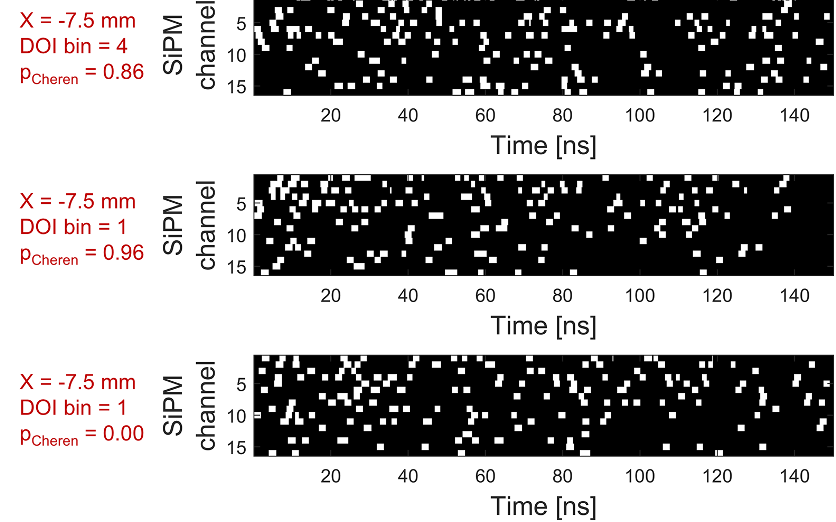
\includegraphics[width=0.9\linewidth]{img/lee2026-bitstream.png}
\end{center}

\paragraph{Why it matters here}
The temporal axis is the direction the notes keep marking as open after
\ref{note:Thull2026} and \ref{note:Carra2022}: cardinality and interaction
order from the joint pattern of per-channel arrival times. This detector
produces exactly that pattern --- their discussion of Figure 10 calls it ``video-like
frames of photon arrivals'' --- and the paper spends it on one number, the
interaction time. Every event is assumed to be one interaction; Compton
scatter inside the slab is never mentioned, and the FPDDs are calibrated with
the same assumption, so a two-site event is fitted as one voxel. Position
again informs timing, the direction \ref{note:Carra2022} runs; nobody runs
the arrival pattern back into position or cardinality.

The FPDD is also the measured counterpart of the \ref{note:Cates2015} PDF: an
arrival-time density per interaction voxel and per channel, with the
Cherenkov and scintillation parts separated. That is the likelihood a Fisher
information calculation needs, so this group has built the ingredients of
both the temporal-axis estimator and its bound without assembling either.
\aside{Their stated next steps are a stacked-slab module and a fully
time-based readout; a multi-interaction analysis is not among them.}

\end{papernote}

\end{programnote}

\begin{programnote}{Prism-PET -- Stony Brook and Weill Cornell, Goldan group}{PrismPET}
\location[251,-80]{40.91}{-73.12}{Stony Brook, New York, USA}
\thumb{img/prismpet.png}

Amir Goldan's group, Stony Brook University, with Weill Cornell Medicine on
every paper since 2023. Single-ended readout of segmented LYSO arrays with a
segmented light guide --- an array of prismatoids --- in place of the uniform
glass slab.

\paragraph{What it is}
The leading light-guide approach to DOI encoding. The mechanism is deliberate
rather than statistical: each prismatoid redirects light into a defined set of
neighbouring readout pixels, so the light-sharing pattern mimics dual-ended
readout while keeping one readout face, and crystal identification improves
rather than degrades. The programme has carried it from a module to a conformal
brain scanner and then to tapered crystals.

\paragraph{Current work}
Goldan's lab (XEIL) is now in Radiology at Weill Cornell Medicine, where
Prism-PET is its main brain project: a compact, portable, upright brain
scanner with motion compensation and CT-less attenuation correction. In
November 2024 Goldan and Gloria Chiang received a \$6.2M U01 from the National
Institute on Aging for it, titled ``High resolution, cost-effective, portable,
and upright brain PET scanner for early diagnosis of Alzheimer's disease''.
Others are taking the design up: a KU Leuven report reads Prism-PET from both
ends and gets \mm{2.57} DOI and \ps{254} CTR at 4-to-1 coupling, \mm{4.01} and
\ps{267} at 9-to-1 --- no better DOI than the single-ended
\ref{note:LaBella2020}. No 2025--26 journal papers from the group were found;
output may be in SNMMI and NSS/MIC abstracts.
\gap{The KU Leuven report's authors and date
(lirias.kuleuven.be/retrieve/fae36454-d553-4745-ac51-ea8f2a6b1669); a 2024
Monte Carlo study of light transport in prismatoid guides (PMC11025681),
whose authors, DOI and the geometry it varies are unchecked --- it may already
sweep the guide shape; and the grant's clinical target (reported elsewhere as
early tau imaging), which the Weill Cornell pages do not state.}

\paragraph{Why it matters here}
This is the design the bulk-scattering mechanism competes with, and the
comparison is the sharpest one available because both answer the same question
--- how to get DOI out of a single readout face --- by shaping where the light
goes rather than by adding a second photosensor. Prism-PET shapes it with
geometry at the far face; this thesis shapes it in the bulk. Their
\ref{note:Zeng2024} result matters most: an optical photon time-of-flight depth
estimate, which is the optical transfer function read out directly in the time
domain rather than through a light-distribution centroid.
\aside{The honest framing is that their encoding is deterministic and mine is
statistical, which is a disadvantage on resolution and an advantage on
manufacturability. Do not pretend otherwise.}

The same determinism is their claim on multi-interaction events, and it is
prior art this thesis must cite. Every interaction lights a fixed pattern of
primary and nearest-neighbour SiPMs, so overlapping patterns from a
multi-crystal Compton event ``can be very accurately decomposed to yield
crystal-level energy, spatial, and DOI information of the individual
interactions'' (\ref{note:Zeng2023}); \ref{note:LaBella2020}'s Supplemental
Note 2 decomposes side-by-side scattered-photon and recoil-electron events,
the most common and hardest case. A uniform light guide, or a monolith, gives
no fixed pattern to decompose against --- which is the difficulty this thesis
takes on. Yet both the scanner and the oTOF papers reject inter-crystal
scatter rather than use it.
The decomposition is \ref{note:Petersen2020}, taken to the whole photopeak in
\ref{note:Petersen2024}: it separates the interactions and picks the first
crystal (64.7\% of scattered events, in simulation), but never orders them in
time.
\gap{Still unread: LaBella 2020's Supplemental Note 2; Makek et al.\ 2019,
``Scintillator pixel detectors for measurement of Compton scattering'',
Condens.\ Matter 4:24. Petersen cites the Davis layered detector as the
complex alternative (``multi-layer, detector with 4-sided readout''); its simulation study is \ref{note:Peng2019}.}

\paragraph{Detector lineage}
Polished LYSO arrays coupled 4-to-1 or 9-to-1 to \qtyproduct{3 x 3}{\milli\metre}
SiPM pixels, prismatoid light-guide array on the non-readout face, \mm{20}
thick throughout.

\paragraph{Scope boundary}
A segmented array, not a monolith --- it belongs on this map as a DOI-encoding
programme, not as a monolithic one, and the review entry should say so.

\begin{papernote}{LaBella et al.\ 2020 -- High-resolution depth-encoding PET detector module with prismatoid light-guide array}{LaBella2020}
\thumb{img/labella2020.png}
J.\ Nucl.\ Med.\ 61(10):1528--1533, \doi{10.2967/jnumed.119.239343}.

\paragraph{Summary}
The module paper that introduced the prismatoid light guide, measured against a
uniform glass light guide built the same way. Flood histograms were taken with
a \MBq{3} \textsuperscript{22}Na source and DOI resolution from lead-collimated
irradiation at known depths.

\paragraph{Key findings}
\begin{itemize}
	\item The uniform glass light-guide module gave DOI resolution \mm{5.0}
		FWHM and energy resolution \qty{13}{\percent} FWHM.
	\item The 4-to-1 coupled Prism-PET module gave DOI resolution \mm{2.5}
		FWHM and energy resolution \qty{9}{\percent} FWHM --- a factor of two in
		DOI from the light guide alone. Both from one centre crystal per
		module; both energies after DOI correction (20\% and 14\% before).
	\item Crystal separation in the flood histogram is uniform across the
		Prism-PET array, where the uniform glass module degrades at the edges
		and corners.
\end{itemize}

\paragraph{The number to take}
\mm{2.5} FWHM DOI at \mm{20} thickness with single-ended readout, with the
edge-and-corner uniformity as the second claim. The uniformity is the one that
is hard to match statistically, because an edge crystal in a monolith sees a
truncated light distribution no matter what the bulk does.

The paper also stakes the Compton claim: a uniform guide gives each event a
random SiPM pattern, the prismatoids a deterministic one wherever the
interaction sits in the column, which lets side-by-side scattered-photon and
recoil-electron events be decomposed into their energies, positions and DOI
(Supplemental Note 2). Inter-crystal scatter recovery is listed among the
design's sensitivity gains, not shown in the main text.

\end{papernote}

\begin{papernote}{LaBella et al.\ 2021 -- Sub-2 mm depth of interaction localization in PET detectors with prismatoid light guide arrays and single-ended readout using convolutional neural networks}{LaBella2021}
\thumb{img/labella2021.png}
Med.\ Phys.\ 48(3):1019--1025, \doi{10.1002/mp.14654}.

\paragraph{Summary}
The Prism-PET module of \ref{note:LaBella2020} --- a 16 x 16 array of
\qtyproduct{1.4 x 1.4 x 20}{\mm} polished LYSO, 4-to-1 on 3~mm SiPMs, BaSO$_4$
between crystals --- with a shallow CNN in place of the ratio estimator for
depth. Depth-collimated data at 19 depths (\mm{1} steps, \mm{1} pinhole),
TOFPET2 readout. Inter-crystal Compton events are cut first by the expected
light-sharing pattern (highest signal over twice the second, second within 1.2
times the third), leaving about 60\% of photopeak events. The CNN is tested on
crystals it was not trained on.

\paragraph{Key Findings}
\begin{itemize}
	\item DOI \mm{1.84} FWHM averaged over the array with all 64 signals, against
		\mm{3.04} for the classical max-over-sum ratio; \mm{1.92} from only the
		four highest signals.
	\item By region with four signals: \mm{1.84} centre, \mm{2.14} edge,
		\mm{2.55} corner (classical 2.59, 4.51, 4.38). The CNN is best at both
		crystal ends, where the ratio estimator is worst.
	\item No SiPM saturation correction; the authors suggest the CNN learns it.
		Energy resolution 8.7\% FWHM, read from Fig.\ 2(a) only (10\% for the
		reference module); timing is not reported.
\end{itemize}

\paragraph{Why it matters here}
The best reported single-ended DOI at \mm{20}, and the number on the
leaderboard a thick monolith or scattering bulk has to approach. It is a
clean-event figure: 40\% of the photopeak, the multi-crystal part, is removed
before it is measured.

\end{papernote}

\begin{papernote}{Zeng et al.\ 2023 -- A conformal TOF-DOI Prism-PET prototype scanner for high-resolution quantitative neuroimaging}{Zeng2023}
\thumb{img/zeng2023.png}
Med.\ Phys.\ 50(6):3401--3417, \doi{10.1002/mp.16223}.

\paragraph{Summary}
The programme's scanner: a decagon-shaped, brain-dedicated single-ring
prototype built from 40 Prism-PET modules, evaluated on DOI, energy, timing and
spatial resolution, sensitivity, and ultra-micro Derenzo and 3D Hoffman
phantoms.

\paragraph{Detector}
Long diameter \cm{38.5}, short diameter \cm{29.1}, axial field of view
\mm{25.5}; each module a 16 x 16 array of
\qtyproduct{1.5 x 1.5 x 20}{\milli\metre} LYSO coupled 4-to-1 to an 8 x 8 SiPM
array with the prismatoid guide opposite.

\paragraph{Key findings}
\begin{itemize}
	\item DOI resolution \mm{2.85} FWHM, DOI-corrected energy resolution
		\qty{12.6}{\percent}, timing resolution \ps{271} FWHM.
	\item Intrinsic spatial resolution \qtyrange{0.89}{1.40}{\milli\metre} FWHM,
		averaging \mm{1.22}; reconstructed resolution \mm{1.53} FWHM across the
		field of view with 3D filtered back-projection.
	\item Peak absolute sensitivity \qty{1.2}{\percent} over a
		\qtyrange{400}{650}{\kilo\electronvolt} window.
	\item \mm{1.00} diameter hot rods fully resolved in the ultra-micro Derenzo
		phantom, which they claim as the highest reported spatial resolution for
		a human brain PET scanner.
\end{itemize}

\paragraph{Why it matters here}
The benchmark a monolithic brain insert gets compared against, and the set of
numbers to quote when the thesis argues what DOI resolution is worth at the
image level. Note the gap between \mm{1.22} intrinsic and \mm{1.53}
reconstructed, which they attribute to mechanical misalignment of detector
blocks rather than to the detector.

Inter-crystal scatter is identified from its characteristic energy pattern
across the SiPMs under one prismatoid and rejected before reconstruction; DOI
rebinning then reassigns each line of response by its continuous depth. The
discussion counts the cost: about half of singles Compton-scatter in
\mm{1.5} crystals, so rejecting them costs much of the sensitivity, and it claims the
overlapping patterns could instead be decomposed to recover the first
interaction --- not done here.

\end{papernote}

\begin{papernote}{Zeng et al.\ 2024 -- Depth-encoding using optical photon TOF in a Prism-PET detector with tapered crystals}{Zeng2024}
\thumb{img/zeng2024.png}
Med.\ Phys.\ 51(6):4044--4055, \doi{10.1002/mp.17095}.

\paragraph{Summary}
The one to read first. A light-sharing module generates several timestamps per
gamma event, and the difference between timestamps from photons travelling in
opposite directions is a depth-dependent optical photon time of flight (oTOF).
The paper's argument is that light leak at the crystal--readout interface is
what destroys this signal, and that tapering the crystal to sit inside the SiPM
active area recovers it.

\paragraph{Detector}
16 x 16 array of \qtyproduct{1.5 x 1.5 x 20}{\milli\metre} LYSO tapered to
\qtyproduct{1.2 x 1.2}{\milli\metre} at the readout face, coupled 4-to-1 to an
8 x 8 array of \qtyproduct{3 x 3}{\milli\metre} SiPM pixels, prismatoid guide
opposite, barium sulphate reflector at \mm{0.1} intercrystal spacing. Scanner
sensitivities were simulated in GATE.

\paragraph{Key findings}
\begin{itemize}
	\item oTOF-based DOI resolution \mm{5.42} FWHM tapered against \mm{13.87}
		FWHM non-tapered --- the first experimental report of oTOF depth
		encoding at module level.
	\item Energy-based DOI resolution \mm{2.35} against \mm{3.18} FWHM for
		centre crystals (tapered edge and corner: 3.70 and \mm{4.76}; \mm{2.68}
		weighted over the module), so tapering improves the conventional
		estimator as well. Energy resolutions are uncorrected for saturation.
	\item Energy resolution \qty{8.88}{\percent} against
		\qty{11.18}{\percent} FWHM; coincidence timing \ps{243} against
		\ps{286} FWHM.
	\item Simulated sensitivity for a 10-ring scanner
		\qty{29.5}{\kilo cps\per\mega\becquerel} tapered against
		\qty{30.9}{\kilo cps\per\mega\becquerel} non-tapered --- the geometric
		cost of tapering is small.
\end{itemize}

\paragraph{Why it matters here}
This is the optical transfer function measured in the time domain, by the
programme that encodes DOI geometrically. The \mm{5.42} against \mm{13.87}
comparison is a direct measurement of how much an interface imperfection
degrades a transfer-function-based estimator, which is the same sensitivity
this thesis has to quantify for bulk scattering --- and it is far larger than the
energy-based estimator's degradation over the same change. That asymmetry is
the finding, and it is an argument for caution about time-domain encoding.
The arithmetic holds --- oTOF DOI degrades by a factor 2.6 between tapered and
non-tapered, the energy estimate by 1.35 --- and it is not confounded by
reflector spacing: tapered and \mm{1.5} cuboid share the same \mm{0.1}
BaSO$_4$ gaps. The comparison has a third arm that settles it. The \mm{1.5}
cuboid crystals overhang the SiPM active area by \mm{0.05} on two sides, and
that leak is the damage; the group's older \mm{1.4} cuboid module, with
\mm{0.2} gaps and crystals inside the active area, gives \mm{2.59} energy and
\mm{6.45} oTOF DOI, close to the tapered \mm{2.35} and \mm{5.42}. The
correlation between the two depth estimates tells the same story: 0.80, 0.43
and 0.83. oTOF is the difference between the primary SiPM's timestamp and its
nearest neighbours'; averaging three neighbours gives the \mm{5.42}, and
combining it with the energy estimate (0.2/0.8) reaches \mm{2.25} for centre
crystals (0.3/0.7 is best at the edges and corners; \mm{2.52} weighted over the
module), so time adds
a little to light here. Inter-crystal scatter is rejected first, so the
timestamps always come from one interaction.

\end{papernote}

\begin{papernote}{Petersen et al.\ 2020 -- Compton decomposition and recovery in a Prism-PET detector module}{Petersen2020}
\thumb{img/petersen2020.png}
IEEE NSS/MIC 2020, \doi{10.1109/NSS/MIC42677.2020.9507898}. Petersen, LaBella,
Howansky, Zhao, Goldan.

\paragraph{Summary}
The multi-interaction paper of the programme, in simulation. A 16 x 16 array of
\qtyproduct{1.4 x 1.4 x 20}{\mm} LYSO on an 8 x 8 SiPM array with the prismatoid
guide; GATE for the gammas, TracePro for the optics. Hits are grouped by
crystal, crystals under \keV{30} dropped, and each firing crystal mapped to its
own SiPM pattern from its energy-averaged depth; the readout is the sum of
those patterns. Two decoders. An analytic one, for central events inside one
prism (about half the photopeak): the ratios of the brightest SiPM signals count
the firing crystals, and a linear system, closed with empirical light-sharing
ratios, splits the pattern into per-crystal energies. And a U-Net-style CNN
that maps the whole 8 x 8 readout to the first interaction position: crystal
index in $x$, $y$ and continuous depth.

\paragraph{Key Findings}
\begin{itemize}
	\item Only 37\% of photopeak events are single-crystal at \mm{1.4} pitch.
	\item Analytic: firing crystals identified 99.3\% correctly (99.7\% one,
		98.9\% two, 88.0\% three or four); decomposed crystal energy off by
		\keV{0.7}, \keV{29.7} and \keV{25.7} on average.
	\item CNN: first-interaction crystal right for about 98\% of single- and
		88\% of multi-crystal events; depth error \mm{1.0} FWHM single,
		\mm{2.1} multi.
	\item Central beam at normal incidence only; edges, corners and oblique
		angles are future work. No timing, no measured data.
\end{itemize}

\paragraph{Why it matters here}
The closest prior art to the multi-interaction half of this thesis, and the
contrast is exact. It separates and counts interactions and recovers the first,
but only because the light guide gives every crystal a fixed, known pattern and
the readout is a linear sum of them --- a dictionary to decompose against. The
first position comes out of the CNN directly; no order is ever estimated, and
energies and patterns are all it uses. A monolith or a scattering bulk has no
such dictionary: each interaction's pattern depends continuously on where it
is, so the decomposition becomes a joint estimate of positions, which is where
arrival times and a bound earn their place. Within one crystal it also merges
all hits to one energy-averaged depth, so it cannot see the multi-site events
inside a crystal that a monolith is made of.

\end{papernote}

\begin{papernote}{Petersen et al.\ 2024 -- Resolving inter-crystal scatter in a light-sharing depth-encoding PET detector}{Petersen2024}
\thumb{img/petersen2024.png}
Phys.\ Med.\ Biol.\ 69:035024, \doi{10.1088/1361-6560/ad19f1}. Petersen,
LaBella, Li, Wang, Goldan --- Stony Brook and Weill Cornell.

\paragraph{Summary}
The journal follow-up to \ref{note:Petersen2020}, still a simulation: GATE
(Penelope physics, \mm{0.1} cuts) for the gamma interactions and TracePro for
the light, with each crystal's light pattern tabulated in 80 depth bins of
\mm{0.25}, on the 1.4 mm, 4-to-1, \mm{20} Prism-PET module. The simulation is
checked against measurement: its block DOI of \mm{2.67} and depth-corrected
energy resolution sit inside the measured 2.50--\mm{3.41} and 8.5--12.6\%
(\ref{note:Zeng2023}, \ref{note:LaBella2020}). Real sensor data are left to
future work, which the authors call the major limitation.

\paragraph{Key Findings}
\begin{itemize}
	\item \textbf{Two adjacent crystals, decoded.} A Bayesian estimate --- a
		scatter-absorption prior times a detector-response likelihood ---
		splits the energy and depth of each crystal to \keV{20.5} and
		\mm{3.1} FWHM error; a small network matches it (\keV{26.2},
		\mm{2.9}). Without the prior, maximum likelihood still works with
		errors about doubled: the response model, that is the light guide,
		carries the accuracy. Their derived prior differs markedly from plain
		Klein--Nishina.
	\item \textbf{Whole photopeak.} A CNN that predicts the first crystal and its
		depth separately: 83.0\% crystal accuracy overall --- 100\% for
		photoelectric events, 64.7\% for inter-crystal scatter, falling from
		65.6\% at the centre to 54.9\% in corners. DOI error \mm{2.4} for
		photoelectric events, \mm{4.2} for scatter, \mm{3.0} for all.
		Photoelectric events are 51.8\% of the photopeak.
	\item \textbf{Image level.} Between two opposed modules \cm{34} apart,
		spillover into the wrong line of response falls from 63.8\% to 47.0\%
		(15.6\% for an ideal detector); the coincidence FWHM goes from 0.82 to
		\mm{0.75} (\mm{0.72} ideal), reported as a 38.9\% improvement on Lee and
		Lee's metric. Simulated hot-rod images resolve \mm{0.8} rods better.
	\item Claims the highest crystal-selection accuracy reported for a
		light-sharing detector, against 73\% in \ref{note:Lee2021}'s comparable
		module.
\end{itemize}

\paragraph{Why it matters here}
The best answer yet to Prism-PET's discarded scatter, and still only a
simulation. It recovers the first crystal for two of three scattered events from
light patterns and energies alone, with no timing --- and the miss rate on
scattered events, about one in three, is the room an arrival-time estimate has
to work in (\ref{note:IdeaOrdering}). Within a crystal it still keeps one
energy-weighted depth, so multi-site events inside one crystal stay merged.
\end{papernote}

\end{programnote}

\begin{programnote}{Crystal Clear and Milano-Bicocca -- light sharing, recirculation and the timing limit}{CrystalClear}
\location[767,-833]{46.23}{6.05}{CERN, Geneva, Switzerland}

Marco Pizzichemi, Stefan Gundacker, Etiennette Auffray and colleagues, spanning
the CERN Crystal Clear collaboration and the University of Milano-Bicocca ---
one group with two addresses, pinned here at CERN.

\paragraph{What it is}
The programme that made light sharing a designed mechanism with a theory
attached. Their modules obtain continuous DOI from a single readout side by
sharing and redirecting scintillation light between neighbouring detectors and
exploiting its attenuation along the crystal, without one-to-one coupling, and
the same group then pushed the coincidence timing of such modules towards the
limit and derived what the timing signal itself can say about depth.

\paragraph{Why it matters here}
Three things this thesis needs come from here. The
light-sharing-and-recirculation mechanism is the conceptual ancestor of every
single-ended DOI design including \ref{prog:PrismPET}'s prismatoids. The
\ps{157} result answers the standard objection to spending light on depth, but
not the way the abstract suggests: sharing the light roughly doubles the raw
timing for the 8 x 8 module (x1.4 for the 4 x 4),
and it is the depth estimate that wins it back by pooling every SiPM's
corrected timestamp (\ref{note:Pizzichemi2019}) --- depth pays for itself
rather than coming free. And \ref{note:LoignonHoule2021}
derives a Cramér--Rao lower bound for time-based DOI estimation, which is the
closest published relative of this thesis's own bound work and has to be cited
as prior art rather than discovered late.

\paragraph{People}
Marco Pizzichemi (first author on the light-sharing line, at both CERN and
Milano-Bicocca), Stefan Gundacker, Etiennette Auffray, Francis Loignon-Houle,
Roger Lecomte.
\gap{Confirm current affiliations --- Gundacker has moved to \ref{prog:Aachen}
and Loignon-Houle's line runs through Sherbrooke, so the group boundary is
softer than one pin suggests. Decide whether Milano-Bicocca deserves its own
panel.}

\begin{papernote}{Pizzichemi et al.\ 2016 -- A new method for depth of interaction determination in PET detectors}{Pizzichemi2016}
\thumb{img/pizzichemi2016.png}
Phys.\ Med.\ Biol.\ 61(12):4679--4698, \doi{10.1088/0031-9155/61/12/4679}.

\paragraph{Summary}
The method paper. Continuous DOI from single-side readout, obtained by sharing
and redirecting scintillation light among several detectors together with the
attenuation of light along the crystal length, and without requiring
one-to-one coupling between scintillators and photosensors. A prototype module
coupling a LYSO matrix to a commercial SiPM array was built and characterised.

\paragraph{Detector}
An 8 x 8 matrix of \qtyproduct{1.53 x 1.53 x 15}{\mm} LYSO at \mm{1.6} pitch,
ends polished and lateral faces mildly depolished, with \um{70} ESR foils
between crystals (not bonded, so an air gap remains). Four crystals share each
\qtyproduct{3 x 3}{\mm} SiPM of a 4 x 4 Hamamatsu array at \mm{3.2} pitch.
On the far face a \mm{1} glass light guide backed by ESR: the light leaving a
crystal's far end is reflected back into the whole matrix and spreads over all
16 SiPMs. A reference module is identical but fully polished, with no light
guide.

\paragraph{Method}
The crystal comes from Anger logic, $(u, v)$, on the 16 signals; the depth from
$w = p_{\max}/P$, the light on the directly coupled SiPM over the total.
Depolishing makes the near-to-far light ratio depend on depth, and the light
guide turns the far share into a spread over every SiPM, so $w$ falls as the
interaction moves away from the sensor. $w$ is linear in depth for every
crystal, calibrated by electronic tagging. Events depositing in more than one
crystal fall away from the 64 clusters in $(u, v, w)$ and are discarded as
``not useful in a realistic PET system''.

\paragraph{Key findings}
\begin{itemize}
	\item Mean DOI resolution \mm{4.1 \pm 0.1} FWHM on \mm{15} long crystals,
		uniform across the array.
	\item Averages over the 16 central crystals. Light output 8800 against 9100
		ADC channels for the polished
		reference, about 3\% lower: that is the ``negligible light loss''.
		Energy resolution is not: raw, 16.1\% against the reference's
		11.2\%, blamed on depolishing and the light guide's absorption. The
		headline 12.7\% is after a depth-dependent gain correction using $w$,
		while the reference figure is uncorrected.
	\item Every crystal separated: excellently in the centre, less
		efficiently near the edges (\S4.1; the abstract says ``all'').
	\item Preliminary coincidence time resolution \ps{353 \pm 7} FWHM, about
		\ps{30} worse than the reference --- derived, not direct: one SiPM
		channel biased, time corrected by a ToT--DOI relation, the reference's
		\ps{155} subtracted and the result scaled by $\sqrt{2}$.
\end{itemize}

\paragraph{Why it matters here}
``Sharing and redirection, plus attenuation along the crystal'' is the
mechanism statement this thesis is a variant of, and it is the earliest clean
one. The claim that depolishing costs negligible light is worth checking
carefully, because it is the same claim a scattering bulk has to make and the
same objection it has to answer.
So the claim holds for light output and not for energy resolution: depth
encoded by depolishing costs spectral sharpness, which a correction recovers
only partly. A scattering bulk has to answer the same split --- total light
kept, but how is it distributed event to event. And the multi-crystal events
are thrown away by construction, which is the opposite of what this thesis
wants to do with them.

\end{papernote}

\begin{papernote}{Pizzichemi et al.\ 2019 -- On light sharing TOF-PET modules with depth of interaction and 157 ps FWHM coincidence time resolution}{Pizzichemi2019}
\thumb{img/pizzichemi2019.png}
Phys.\ Med.\ Biol.\ 64(15):155008, \doi{10.1088/1361-6560/ab2cb0}.

\paragraph{Summary}
The timing follow-up: the same light sharing and recirculation mechanism
examined with timing as the focus, together with a method that uses the DOI
information to optimise coincidence time resolution. A dedicated 64-channel
readout with \ps{16} FWHM intrinsic timing resolution was built for it.

\paragraph{Method}
Eight modules: depth-encoding (depolished, glass light guide) and polished
references, each as an 8 x 8 matrix of \mm{1.53} crystals or a 4 x 4 of
\mm{3.1}, all \mm{15} long on 4 x 4 arrays of \mm{3} SiPMs read through
NINO32. Timing uses every SiPM, not only the one under the crystal: light
reaching the others is delayed by an amount that depends on depth, so each
measured delay $g_i(w) = \langle t_i - t_1 \rangle$ is calibrated against $w$,
every SiPM yields its own estimate $t_1^{(i)} = t_i - g_i(w)$, and the
estimates are averaged with weights $1/\sigma_i^2$. The thumbnail is one such
delay against $w$.

\paragraph{Key findings}
\begin{itemize}
	\item \ps{157} FWHM coincidence time resolution, with \mm{1.5} FWHM spatial
		resolution, \mm{3} FWHM DOI resolution and \qty{9}{\percent} FWHM energy
		resolution at \keV{511}, on \mm{15} long crystals.
	\item The \ps{157} is the central crystals of the 8 x 8 module after
		correction (\ps{166} over all crystals; the 4 x 4 gives 159 and 165).
		Before correction the same modules give \ps{307} (8 x 8) and \ps{233}
		(4 x 4), against \ps{154}--\ps{162} for the polished references.
	\item Extracting the DOI coordinate was shown not to deteriorate the
		module's timing performance.
	\item The readout's own contribution is \ps{16} FWHM, so the quoted CTR is
		a detector number rather than an electronics one.
\end{itemize}

\paragraph{The claim to be substantiated}
That DOI extraction is free in timing terms. The full text says something more
precise and more useful. The light-sharing module's raw timing is twice the
reference's --- sharing the light \emph{does} cost the timestamp --- and it is
the depth estimate that buys it back, by telling each SiPM's delay so that all
16 timestamps can be pooled. Corrected, the depth module matches the polished
one; so depth is not free, it is the price of recovering what light sharing
spent. That pooling is a depth-informed combination of per-channel arrival
times: a first, single-interaction step along the temporal axis.

The figures in the abstract are not one measurement. Timing and energy (8.9\%
central) are measured here; the \mm{3} DOI is cited from Stringhini et al.\
2016, and the \mm{1.5} is the positron-range limit the \mm{1.53} crystals are
argued to reach (pitch \mm{1.6}), not a measurement. The \ps{157}, like every
CTR in its Table 2, is fitted against a reference crystal, the reference
subtracted and the result scaled by $\sqrt{2}$.

\end{papernote}

\begin{papernote}{Loignon-Houle et al.\ 2021 -- DOI estimation through signal arrival time distribution: a theoretical description including proof of concept measurements}{LoignonHoule2021}
\thumb{img/loignonhoule2021.png}
Phys.\ Med.\ Biol.\ 66(9):095015, \doi{10.1088/1361-6560/abf604}.

\paragraph{Summary}
The paper this thesis has to engage with. Fast timing signals intrinsically
carry DOI information even with single-ended readout, so features of the
detected photon arrival-time distribution can be used to estimate where the
interaction happened --- and in return improve timing precision. The argument is
made in two steps: measurements with LSO:Ce:Ca on FBK NUV-HD SiPMs and
high-frequency readout, establishing a DOI effect on CTR not visible with
slower electronics and a double-threshold DOI discrimination scheme; then a
simulation study of four estimators for future detectors.

\paragraph{Key findings}
\begin{itemize}
	\item \textbf{Measurement:} a \qtyproduct{2 x 2 x 20}{\mm} LSO:Ce:Ca
		crystal on a \qtyproduct{4 x 4}{\mm} FBK NUV-HD SiPM, high-frequency
		readout, scanned at six depths against a \mm{3} reference. CTR is
		worst mid-crystal even though light output rises towards the SiPM ---
		not the $1/\sqrt{N}$ behaviour light alone predicts.
	\item A DOI-dependent effect on coincidence time resolution is resolvable
		with high-frequency readout and was not observable with slower
		electronics.
	\item A double-threshold scheme on the analogue timing signal, combined
		with signal intensity, discriminates DOI with no detector modification
		and no complex readout: \mm{8.5 \pm 0.4} DOI resolution, or about 90\%
		correct top-half against bottom-half.
	\item A simple two-timestamp difference estimator improves CTR; kernel
		density estimation and a neural network do better and converge to the
		bound.
	\item The paper derives a Cramér--Rao lower bound for time-based DOI
		estimation. The tested estimators, KDE especially, come close to it,
		so a better estimator would gain little; a larger gain needs a detector
		whose time profile changes more with depth. Uncorrected, CTR saturates
		at 60--\ps{70} for a \mm{20} crystal; with DOI correction and
		\ps{10} SPTR the simulated detectors reach about \ps{10}.
\end{itemize}

\paragraph{The bound}
From section 2.2.8.
\begin{itemize}
	\item \textbf{Likelihood.} Each detected photon's time is an
		independent draw from one density $p_{\mathrm{tot}}(t \mid d)$, the
		convolution of emission (one bi-exponential), transport at depth $d$
		and a Gaussian SiPM response. Per-photon Fisher information
		$\mathcal{I}(d) = \int (\partial_d p_{\mathrm{tot}})^2 /
		p_{\mathrm{tot}}\,\mathrm{d}t$, and the bound is
		$\mathrm{Var}(\hat{d}) \geq 1/(N_d\,\mathcal{I}(d))$ with $N_d$ the
		\emph{expected} number of detected photons.\aside{ Photons are
		treated as i.i.d.\ and unordered, though the estimators use ordered
		first-$n$ timestamps, and the photon count is fixed rather than
		Poisson, so depth information in the count itself is left out.}
	\item \textbf{Per event.} It bounds a single event's depth from its
		$N_d$ photons; it is the usual i.i.d.\ CRLB, attained only
		asymptotically in $N_d$. To turn it into a CTR they draw each event's
		depth from a normal with that variance and push it through the same
		time-bias correction as the real estimators.
	\item \textbf{Nuisance.} The gamma's arrival time $\theta$ is the only
		one, and it is not profiled but removed: each depth's density is
		shifted so all start together, on the argument that the first trigger
		alone should say nothing about depth.\aside{ That alignment discards
		the absolute-onset information a joint $(\theta, d)$ treatment would
		handle through the Schur complement.}
	\item \textbf{Same detector?} No, in two ways. The measured detector
		(analogue SiPM, double threshold) is not the simulated one (a
		\mm{20} polished crystal, 98\% specular reflector, digital SiPM
		timestamping every photon, PDE 55\%, no dark counts). And within the
		simulation, the estimators' transport densities come from Geant4 while
		the bound's come from the analytic model of \ref{note:Cates2015}.
	\item \textbf{Single interaction.} Only photoelectric events are
		simulated and kept. The authors say outright that multi-interaction
		events --- ``Compton interaction followed by a photoelectric
		interaction in the same crystal'' --- are ``a complex problem worthy of
		future investigation, especially for monolithic crystals'', and that
		energy and depth are confounded in the timestamps: a low-energy deep
		event can look like a high-energy shallow one.
\end{itemize}

\paragraph{Why it matters here}
This is prior art for the bound work, and it must be cited as such. The
difference to establish is one of parameterisation: their bound is on DOI
estimated from the arrival-time distribution in a clear crystal, where the
depth dependence comes from optical path length; the bound this thesis needs is
on position estimated from a scattering bulk, where the depth dependence is
engineered into the spatial light distribution as well. The Fisher information
is computed from a different observable, and that has to be said explicitly and
early.
The full text sharpens the difference into three points to make in the
chapter: their observable is the time of each photon and nothing else
(positions, counts per channel and energy are all outside the likelihood);
their nuisance handling is an alignment, not a profile; and their model is one
interaction per event, which they name as the open problem for monoliths.
\aside{Finding this late would have been bad. It is the single most important
citation on this map for the CRLB chapter.}

\end{papernote}

\end{programnote}

\begin{programnote}{Geneva HUG -- Zaidi group, PET system design by simulation}{Geneva}
\location[770,-146]{46.19}{6.15}{Geneva, Switzerland}

\paragraph{What it is}
Habib Zaidi's Division of Nuclear Medicine and Molecular Imaging at Geneva
University Hospital, with Tehran University of Medical Sciences (Mohammad Reza
Ay) on the instrumentation. Monte Carlo design studies of whole scanners, and
deep-learning work across PET; on this map for its monolithic system design.

\paragraph{People}
Habib Zaidi (lead), Amirhossein Sanaat, Hossein Arabi; Mohammad Reza Ay
(Tehran).
\gap{Sanaat's later monolithic positioning work --- the multilayer perceptron
for DOI on a 12 x 12 SiPM array that \ref{note:Shen2025} cites --- is not this
paper; find and note it.}

\begin{papernote}{Sanaat et al.\ 2020 -- Novel preclinical PET geometrical concept using a monolithic scintillator crystal offering concurrent enhancement in spatial resolution and detection sensitivity: a simulation study}{Sanaat2020}
\thumb{img/sanaat2020.png}
Phys.\ Med.\ Biol.\ 65(4):045013, \doi{10.1088/1361-6560/ab63ef}. Sanaat,
Arabi, Ay, Zaidi.

\paragraph{Summary}
Mix thin and thick monoliths in one small-animal ring: \mm{2} blocks for
resolution, \mm{10} blocks for sensitivity, either facing their own kind or
facing each other, with rotating variants to even out the resolution. Rings of
10 or 12 blocks (bores \mm{154} and \mm{187}), each a
\qtyproduct{50.2 x 50.2}{\mm} LYSO monolith in BaSO$_4$ on a 12 x 12 SiPM array
at \mm{4.2} pitch. GEANT4 with full optical transport --- a ``Paint''
reflector at 97\% and UNIFIED ``ground'' crystal--glue--SiPM interfaces, 25{,}000 photons per MeV --- validated against the group's prototype
scanner, and positioned by an analytic row-and-column method (correlated signal
enhancement). No DOI, no learning, simulation only.

\paragraph{Key Findings}
\begin{itemize}
	\item All-\mm{2} rings: 0.6--\mm{0.75} radial, but 1.6--2.6\% sensitivity;
		all-\mm{10}: up to 4.3\%, resolution no better than about \mm{1}.
	\item Mixed rings beat a uniform \mm{6} compromise: \mm{0.6}--\mm{0.9}
		against 0.8--\mm{1.2}, at similar or higher sensitivity (2.8\% for 12
		blocks against 2.45\%), with 40\% less LYSO than the all-\mm{10}
		rings.
	\item Peak NECR 16--20 kcps, lower than the uniform rings and judged
		irrelevant at mouse activities.
\end{itemize}

\paragraph{Why it matters here}
A system-level answer to the same thickness trade a monolith faces --- depth
blurs the thick crystal --- solved by geometry rather than by recovering depth:
the thin side of each line of response pins it. That is the alternative to
measuring DOI, and a reason a thick-monolith thesis has to show its depth
estimate is worth more than simply mixing thicknesses. Two cautions: depth is
ignored outright, which flatters the thick blocks' parallax, and the surfaces
use the UNIFIED ``ground'' model that \ref{note:Roncali2013} shows
overestimates collected light.

\end{papernote}

\end{programnote}

\begin{programnote}{QST Chiba -- Yamaya group, layered DOI and the X'tal cube}{QST}
\location[-68,-351]{35.63}{140.11}{Chiba, Japan}

Taiga Yamaya's group at the National Institutes for Quantum Science and
Technology (formerly the National Institute of Radiological Sciences), Chiba.
The main non-monolithic school of DOI encoding, and the only Japanese programme
on this map.

\paragraph{What it is}
DOI by segmentation rather than by positioning. The group's long-running answer
is to build the depth information into the crystal block itself --- staggered
multi-layer arrays, and in the X'tal cube a three-dimensional array of
\qtyproduct{1 x 1 x 1}{\milli\metre} crystals read out on all six faces
(\ref{note:Yamaya2011}), glued in 2011 and laser-engraved inside a monolithic
block in the versions that followed --- so that depth is recovered by
crystal identification instead of from a continuous light distribution. The
programme also ships: their hemispherical brain scanner is sold in Japan as
VRAIN.

\paragraph{Why it matters here}
The alternative this thesis has to argue against, and the one with the strongest
record. Segmentation gets depth by construction, at the cost of dead material,
assembly complexity and a fabrication step per layer; a scattering bulk gets it
from the optics of a single piece of crystal. A literature review that does not
state that trade-off explicitly has not engaged with the field. The X'tal cube
is the sharpest case, because it starts from a monolith and then removes the
very continuity this thesis depends on.
\aside{Note the irony and use it: the X'tal cube's successors are laser-engraved
inside a monolithic block, a demonstration that the bulk of a monolith can be
structured optically. That is closer to a scattering bulk than it first looks.}

\paragraph{People}
Taiga Yamaya (PI), Han Gyu Kang, Eiji Yoshida, Fumihiko Nishikido, Go Akamatsu.

\paragraph{Off the map: Kang et al.\ 2026}
Kang et al.\ 2026, ``Design optimization using GATE Monte Carlo simulations for a
sub-0.5 mm resolution PET scanner with 3-layer DOI detectors'', Phys.\ Med.\
Biol.\ 71:035001 (doi 10.1088/1361-6560/ae3b02), was noted here and taken off:
it is a layered, not monolithic, detector, and its GATE model has optical
processes switched off --- gamma interactions only, inter-crystal scatter
collapsed to an energy-weighted centroid per layer and then the highest-energy
hit. Its one result worth keeping: the gamma-only model matched measured radial
resolution to \mm{0.03} out to \mm{10} off centre, but missed by \mm{0.3} at
\mm{15}, which the authors put down to crystal-decoding errors in the real
light-sharing readout. A model without optics fails exactly where the light
distribution decides the answer.

\paragraph{To read}
\gap{The laser-processing papers (2012 NSS/MIC, 2013 TNS) and
the VRAIN system paper, Akamatsu et al.\ 2022, Phys.\ Med.\ Biol.\
67(22):225011, \doi{10.1088/1361-6560/ac9e87}, which reports \mm{2.2} rods and
\ps{229} TOF with one-to-one coupling and no DOI --- worth recording as the
commercial outcome even though it is off this map's theme.}

\begin{papernote}{Yamaya et al.\ 2011 -- A SiPM-based isotropic-3D PET detector X'tal cube with a three-dimensional array of 1 mm\textsuperscript{3} crystals}{Yamaya2011}
\thumb{img/yamaya2011.png}
Phys.\ Med.\ Biol.\ 56(21):6793--6807, \doi{10.1088/0031-9155/56/21/003}.
Yamaya, Mitsuhashi, Matsumoto, Inadama, Nishikido, Yoshida, Murayama, Kawai,
Suga, Watanabe --- NIRS, Chiba University, Hamamatsu.

\paragraph{Summary}
A 16 x 16 x 16 block of 4096 LYSO cubes, \mm{0.993} on a side, polished and glued
with no reflector inside, read out on all six faces by 96 Hamamatsu MPPCs (a
4 x 4 array of \qtyproduct{3 x 3}{\mm} per face). Position is one 3D Anger
centroid over all 96 signals; each spot in the 3D flood is a crystal. The
chosen design adds \mm{1} light guides and a thin reflector belt at the edges.
(The abstract says LGSO; the text and tables say LYSO.)

\paragraph{Key Findings}
\begin{itemize}
	\item Almost all 4096 crystals identified; edge planes partly merged.
	\item Energy resolution 12.7\% FWHM; no timing, and no resolution in mm
		--- the isotropic \mm{1} is the crystal pitch.
	\item Inter-crystal scatter is not handled: in simulation 43.6\% of
		events scatter between crystals; the mean positioning error over all
		events is \mm{1.49}; maximum-likelihood recovery is proposed, not done.
	\item Next: laser-engraved grids inside a monolithic block, to cut the
		assembly cost and the faces read out.
\end{itemize}

\paragraph{Why it matters here}
The far end of segmentation: depth by construction at \mm{1} in three
dimensions, at the price of 96 photosensors for a \mm{16} cube and nearly half
the events mispositioned by scatter it does not try to separate.
\end{papernote}

\begin{papernote}{Kang et al.\ 2023 -- Submillimeter-resolution PET for high-sensitivity mouse brain imaging}{Kang2023}
\thumb{img/kang2023.png}
J.\ Nucl.\ Med.\ 64(6):978--985, \doi{10.2967/jnumed.122.264433}. Kang,
Tashima, Wakizaka, Nishikido, Higuchi, Takahashi, Yamaya. Open access.

\paragraph{Summary}
SR-PET: a \mm{52.5} ring of 64 detectors, each three staggered layers of
\qtyproduct{0.9 x 0.9}{\mm} LYSO crystals (4, 4 and \mm{7}; \mm{15} in all),
offset half a pitch so each layer lands at its own spot in one flood map; four
signals per SiPM array. Depth is three discrete bins. Energy 24.3\% system-wide;
timing \ns{9.5}.
\begin{itemize}
	\item Resolution: about \mm{0.6} with 3D OSEM, about \mm{1.0} with FBP,
		at the centre; \mm{0.55} rods resolved at 50 iterations, \mm{0.75}
		rods at 10 (the Inveon fails the \mm{0.75} rods; it was not tested
		on the \mm{0.55} phantom). Resolution figures are averages over
		0--\mm{10} radial offset.
	\item Peak sensitivity 8.66\% at 250--\keV{750}, falling to 2.84\% at
		400--\keV{600} and 1.56\% at 440--\keV{560}: inter-crystal scatter is
		only rejected by narrowing the window.
	\item Parallax still degrades radial resolution at 10--\mm{15} off centre:
		three layers do not remove it.
\end{itemize}

\paragraph{Why it matters here}
The best pixelated DOI preclinical system on this map, and the clearest price
list for it: a 5.5-fold sensitivity loss to keep scatter out, per-crystal
calibration, a 72-hour normalisation. That sensitivity cost is exactly what
recovering multi-interaction events in a continuous crystal would bid for.

\end{papernote}

\end{programnote}

\begin{programnote}{MODE Collaboration -- differentiable detector design}{MODE}
\location[-960,1100]{50.67}{4.61}{Louvain-la-Neuve, Belgium}
 
\gap{\textbf{Entire node unverified.} This is the load-bearing claim of the
thesis pivot and currently has no grounding in this file at all. Fill before
writing any proposal text.}
 
\paragraph{The claim to be substantiated}
Three propositions, each of which needs a citation:
\begin{enumerate}
	\item HEP built end-to-end differentiable / surrogate-based detector design
		machinery between roughly 2022 and 2026. \gap{Which papers, which
		toolchains, which experiments.}
	\item GATE 10 (2025) made the equivalent feasible in medical imaging.
		\gap{See \ref{prog:OpenGATE}.}
	\item The 5th MODE workshop contained zero PET, SPECT or Compton camera
		work. \gap{Verify against the actual programme. A time-bounded absence
		claim is checkable and will be checked --- get the workshop date,
		location, and the full session list, and record where you looked.}
\end{enumerate}
 
\paragraph{Why the third point is the fragile one}
An absence claim is only as good as its search. If a reviewer finds one
PET-adjacent contribution, the framing collapses. Either verify exhaustively and
cite the programme, or reframe as ``substantially absent'' with the evidence
shown.
 
\end{programnote}
 
 
% ===========================================================================
% 9. STUB -- OpenGATE.
% ===========================================================================
 
\begin{programnote}{OpenGATE -- GATE 10}{OpenGATE}
\location[150,1100]{45.76}{4.84}{Lyon, France}
 
\gap{Entire node unverified.}
 
\paragraph{Why it matters}
The stated enabling condition for doing differentiable co-design in medical
imaging rather than HEP. If the argument is ``this became possible in 2025'',
the release, its capabilities, and specifically what it exposes that GATE 9 did
not, all need to be on the record.
 
\gap{Sarrut et al.\ GATE 10 release paper --- full citation, release date, and
the specific feature that enables gradient flow or surrogate training. Also:
does it actually support what the pivot needs, or does it need extending? That
question is the difference between a feasible thesis and an infeasible one.}
 
\end{programnote}
 
 
% ===========================================================================
% 10. STUB -- own group. Uncomfortable but necessary.
% ===========================================================================
 
\begin{programnote}{UTS -- Franklin group}{UTS}
\thumb{img/uts.png}
\location[-900,-600]{-33.88}{151.20}{Sydney, Australia}

\paragraph{What it is}
School of Electrical and Data Engineering, University of Technology Sydney.
Daniel R.\ Franklin (PI), with Mitra Safavi-Naeini and Mehran Abolhasan;
students Keenan Wilson (PhD 2020), Roumani Alabd, Mushen Shen, Ragy Abraham.
Site: \url{https://www.uts.edu.au/staff/daniel.franklin}. The line is a
continuous cylindrical-shell PET scanner in cheap monolithic media ---
nanocomposites and transparent ceramics --- with the localisation done by
networks.

\paragraph{Why it needs to exist}
Two of the seven kills are internal. Writing the external landscape carefully
while leaving the internal one implicit is the failure mode this file exists to
prevent. \gap{Scope boundary: what is Abraham's lane, explicitly, and where
does it end? Ask Franklin directly.}

\begin{papernote}{Li et al.\ 2015 -- A new virtual ring-based system matrix generator for iterative image reconstruction in high resolution small volume PET systems}{Li2015}
\thumb{img/li2015.png}
Phys.\ Med.\ Biol.\ 60(17):6949--6973, \doi{10.1088/0031-9155/60/17/6949}.
Li, Safavi-Naeini, Franklin, Han, Rosenfeld, Hutton, Lerch --- Centre for
Medical Radiation Physics, Wollongong, with UTS and UCL. Filed from the authors'
accepted manuscript (UTS OPUS).

\paragraph{Summary}
A very fine detector makes the system matrix too large to hold. The answer here
is a virtual single-layer detector ring: every physical line of response, from
any detector element and depth, is mapped to the pair of virtual detectors it
crosses, and the matrix is built for those. Two ways to fill it are compared ---
Siddon ray tracing with a detector response, and Monte Carlo --- on PETiPIX, a
simulated mouse-brain scanner of four edge-on Timepix silicon pixel detectors
(\um{55} pixels, a \mm{15} field) that detects mostly by tracking recoil
electrons rather than by photoelectric absorption.

\paragraph{Key Findings}
\begin{itemize}
	\item Compression of $5 \times 10^{7}$ (geometric) and
		$2.5 \times 10^{7}$ (Monte Carlo), leaving 0.5--\qty{1.2}{GB} of
		matrix in memory.
	\item The Monte Carlo matrix gives the best images (contrast recovery,
		noise, structural similarity) at a large one-off cost; MOBY mouse-brain
		structures resolve below a millimetre.
	\item A 3D extension, the virtual cylinder, is shown on a small-animal DOI
		design (\mm{35} across, \mm{30} long).
\end{itemize}

\paragraph{Why it matters here}
The virtual-cylinder method \ref{note:EnriquezMieyTeran2024} tests on the
Sydney mouse scanner, from the same UTS circle as the shell-scanner papers
above; Enríquez calls its comparison of compressed and full matrices
inconclusive and makes that comparison directly. PETiPIX's recoil-electron tracking is also a direct-detection
counterpart to resolving multiple interactions.
\end{papernote}

\begin{papernote}{Wilson et al.\ 2019 -- Localisation of the lines of response in a continuous cylindrical shell PET scanner}{Wilson2019}
\thumb{img/wilson2019.png}
41st IEEE EMBC, Berlin, \doi{10.1109/EMBC.2019.8856676}. Wilson, Alabd,
Abolhasan, Franklin, Safavi-Naeini.

\paragraph{Summary}
A technique for localising LOR endpoints in a PET scanner built from a
continuous cylindrical shell scintillator, demonstrated on a simulated
sensitivity-optimised shell in two materials, the ceramic garnet GLuGAG:Ce and
a LaF\textsubscript{3}:Ce--polystyrene nanocomposite (the abstract says
LuF\textsubscript{3}; the body and Table I say LaF\textsubscript{3}).
\aside{The co-supervisor's own prior art on the capstone geometry.}
Positioning extends Li et al.'s analytic method to a cylindrical shell: a model
of the optical photon distribution, with total-internal-reflection cut-offs, is
fitted jointly to the inner and outer photon maps by Levenberg--Marquardt (GATE
8.1, full optical tracking). Median LOR placement error 1.27--\mm{1.62} for
GLuGAG:Ce and 3.12--\mm{4.13} for LaF\textsubscript{3}:Ce--PS, from the centre
to 75\% of the inner radius.

\end{papernote}

\begin{papernote}{Wilson et al.\ 2020 -- Optimisation of monolithic nanocomposite and transparent ceramic scintillation detectors for positron emission tomography}{Wilson2020}
\thumb{img/wilson2020.png}
Sci.\ Rep.\ 10:1409, \doi{10.1038/s41598-020-58208-y}.

\paragraph{Summary}
A Monte Carlo method for choosing the thickness of a monolithic slab by
maximising the probability of detecting and localising a \keV{511}
interaction, run over five nanocomposites and four ceramics; LaF\textsubscript{3}:Ce--polystyrene
and GLuGAG:Ce reach 48.8\% and 67.8\% sensitivity at the stated localisation
accuracy. The paper that set up the monolithic + NN line.

\end{papernote}

\begin{papernote}{Wilson 2020 -- High-sensitivity PET using optimised continuous cylindrical shell nanocomposite and transparent ceramic scintillators (PhD thesis)}{Wilson2020a}
\thumb{img/wilson2020a.png}
UTS, \href{https://opus.lib.uts.edu.au/handle/10453/147336}{OPUS}.

\paragraph{Summary}
The thesis behind the two papers above, supervised in Franklin's group: a
continuous cylindrical shell of nanocomposite or transparent ceramic scintillator
as a cheaper route to sensitivity, read by SiPMs on both its inner and outer
surfaces, all in GATE with full optical tracking. Chapters 3 and 4 are
\ref{note:Wilson2020} and \ref{note:Wilson2019}; chapters 5 and 6 are not
published elsewhere on this map.

\paragraph{Key Findings}
\begin{itemize}
	\item \textbf{Materials (ch.\ 3).} Five nanocomposites and four ceramic
		garnets; ``optimal thickness'' defined as the one that localises the
		most photons to within a set distance. GLuGAG:Ce is best: about
		\mm{20} for accuracy (46\% of photons within \mm{1}, 62.5\% within
		\mm{5}), about \mm{27.5} for sensitivity. LaF\textsubscript{3}:Ce in
		polystyrene is the best nanocomposite. The position fit needs an extra
		optical-scattering term these materials demand.
	\item \textbf{The shell (ch.\ 4).} A polygonal shell \mm{296} long,
		\mm{233} inner radius, \mm{24.9} thick in GLuGAG:Ce (\mm{42.9} in
		LaF\textsubscript{3}:Ce-PS), 104 inner and 116--124 outer faces of
		\mm{14.2}; detection efficiency 67.8\% and 48.8\%. Median LOR error
		1.27--\mm{1.62} (GLuGAG) and 3.12--\mm{4.13} (nanocomposite) from
		the centre to 75\% of the radius.
	\item \textbf{Pile-up (ch.\ 5).} In one continuous shell, events
		overlap in space and time. Pixels are grouped into regions, each
		region's light flux is deconvolved by the scintillator's
		depth-dependent impulse response into an impulse train marking event
		onsets, and coincidences are pairs of impulses in one timing bin and
		different regions. Of all annihilations, 32.8\% are geometrically
		detectable; the algorithm finds 17.4\%, misses 15.4\% (mostly weak
		signals) and adds 2.1\% randoms. Timing is sampled at \ns{10}, so
		not TOF.
	\item \textbf{Images (ch.\ 6).} A brain scanner reconstructed in STIR
		(2D FBP, 3D FBP with reprojection, OSEM): \mm{2} sources under
		\mm{4} FWHM in nearly every direction with OSEM --- from only
		\qty{3}{\second} of simulated data, since full optical tracking is
		so costly.
	\item \textbf{Future work:} NEMA testing from a statistical model of the
		localisation error instead of full optics; sub-nanosecond, TOF-capable
		timing by joint spatial--temporal pulse analysis; other materials;
		a truncated spherical shell for the brain.
\end{itemize}

\paragraph{Why it matters here}
The group's own starting point for the capstone geometry, and a case of
separating overlapping events in a monolith using time: chapter 5
deconvolves the optical flux in space and time to find event onsets. It works
between events (pile-up), at \ns{10}, not between the interactions of one
event --- the gap this thesis aims at. Its proposed next step, joint
spatial--temporal pulse analysis for timing, points the same way.

\end{papernote}

\begin{papernote}{Shen et al.\ 2025 -- Deep learning based localisation and classification of gamma photon interactions in thick nanocomposite and ceramic monolithic scintillators}{Shen2025}
\thumb{img/shen2025.png}
Sci.\ Rep.\ 15:28607, \doi{10.1038/s41598-025-13339-y}. Shen, Abraham,
Cribbin, Gregor, Safavi-Naeini, Franklin.

\paragraph{Summary}
An InceptionNet classifier for the mode of interaction and CNN and
InceptionNet regressors for the first interaction point, from scintillation
photon distributions in thick monolithic nanocomposite and ceramic slabs.
Single-deposition events classified at $\geq$90.1\%, two-deposition at
$\geq$77.6\%, three-plus at $\geq$66.7\% (abstract; its Table 6 gives 66.4\%); median localisation error
\qtyrange{0.58}{2.91}{\milli\metre} with the CNN and
\qtyrange{0.59}{2.10}{\milli\metre} with InceptionNet.

\paragraph{Method}
GATE simulation of nine thick slabs, five nanocomposites and four ceramics,
each at the optimum thickness from \ref{note:Wilson2020}, read out on both
faces through Meltmount; 50{,}000 gammas per material, trained at 100\%
detector efficiency and evaluated down to lower ones. The input to every
network is the optical photon \emph{count} map on the two faces, 20 x 20 x 2.
GATE records each interaction's time, but no network uses it. The classifier
has three classes --- one, two, or three-plus energy deposits --- and the
localiser one target, the first point of interaction, from a single network
for all events: the class is not fed into positioning.

\paragraph{Key Findings}
\begin{itemize}
	\item \textbf{Classification} is nearly material-independent: one
		deposit 90.1--91.4\% correct, two 77.6--81.7\%, three-plus
		66.4--68.4\%; multi-deposit events are mostly misread as fewer
		deposits, with about a quarter of three-plus events called single.
	\item \textbf{Localisation} at 50\% efficiency: median error
		\mm{0.58} to \mm{1.13} in the ceramics, \mm{0.87} to \mm{2.91} in
		the nanocomposites, where InceptionNet beats the plain CNN by 46\% on
		average; both beat the earlier least-squares fit (LaBr$_3$:Ce/PS
		median \mm{1.2} to \mm{0.87}).
	\item \textbf{Use of the class} is proposed, not done: weight each event
		in the sinogram by its number of deposits, and keep Compton events
		that a photopeak window would drop.
\end{itemize}

\paragraph{Why it matters here}
``Classification'' in the title: interaction multiplicity is already being
classified in this group, so the multiplicity classifier is an inheritance,
not a proposal. What the paper leaves is the rest of the multi-interaction
problem: it counts deposits but locates only the first, never orders them,
never conditions positioning on the count, and never looks at arrival times
--- the input is photon counts alone. So the temporal axis is untouched here
as well as in \ref{note:Decuyper2021} and \ref{note:Lee2026}: this is the
counting half from light, with timing and the later vertices still open.

\end{papernote}

\end{programnote}

% ===========================================================================
% University of Sydney -- Open-Field Mouse Brain PET (Kyme, Meikle). Dual-ended
% multiplexed DOI detectors, in-situ DOI calibration, inter-crystal scatter.
% ===========================================================================

\begin{programnote}{University of Sydney -- Open-Field Mouse Brain PET (Kyme, Meikle)}{USYD}
\location[-68,109]{-33.888}{151.187}{Brain and Mind Centre, University of Sydney}

\paragraph{What it is}
A brain PET scanner for an awake, freely moving mouse: four box-shaped panels of
dual-ended readout DOI detectors around an open field, a gantry that follows the
animal, and motion tracking for motion-compensated reconstruction. Andre Kyme
and Steven Meikle (Brain and Mind Centre and School of Biomedical Engineering)
lead it; Francisco Enríquez-Mier-y-Terán's detector, reconstruction and
calibration papers are the instrumentation; UC Davis (Sun Il Kwon, Martin
Judenhofer) collaborates. Funded by the Australian Research Council
(DP190102318).
\gap{The system papers: Kyme et al.\ 2017 (design optimisation) and the 2021
NSS/MIC overview; whether the full scanner has been built and imaged.}

\paragraph{Why it matters here}
The local, measured case for dual-ended readout: 9:1 multiplexing so the second
photosensor does not double the electronics, a calibration that needs no
collimator, and a simulation study of inter-crystal scatter that puts a
physical ceiling on picking the first interaction. Meikle is also in the near
network, and with Nuyts, Jones and Cherry wrote the 2026 history of the field
(``Landmark developments in nuclear medicine physics and engineering over the
last 70 years'', PMB) the thesis can lean on.

\begin{papernote}{Enríquez-Mier-y-Terán et al.\ 2024 -- Virtual cylindrical PET for efficient DOI image reconstruction with sub-millimetre resolution}{EnriquezMieyTeran2024}
\thumb{img/enriquezmieyteran2024.png}
Phys.\ Med.\ Biol.\ 69:115043, \doi{10.1088/1361-6560/ad4c51} (corrigendum
69:179501). Enríquez-Mier-y-Terán, Kyme, Angelis, Meikle. Open access.

\paragraph{Key Findings}
\begin{itemize}
	\item The box-shaped scanner's lines of response, across crystal pairs and
		DOI bins, are condensed onto a virtual cylinder of detectors
		(0.74, 0.47 or \mm{0.36}), each virtual pair standing for every
		physical line that crosses it. GATE simulation.
	\item At least 50\% fewer lines of response; with \mm{0.47} virtual
		detectors and 6 DOI bins (\mm{3.3} each), 86\% fewer and transaxial
		images nearly identical to the physical geometry's.
	\item Sub-millimetre volumetric resolution across the field with 6 DOI
		bins. Radial and tangential anisotropy follows the DOI resolution, not
		the virtual detector size; the axial direction loses most.
		Resolution modelling removes most of the anisotropy the box geometry
		causes.
\end{itemize}

\paragraph{Why it matters here}
DOI makes the number of lines of response explode in a non-cylindrical,
narrow-bore scanner; this is a practical way to reconstruct one, building on the
virtual ring of \ref{note:Li2015}, and the
geometry problem Prism-PET's decagon (\ref{note:Zeng2023}) and the WT-PET panels
(\ref{prog:WTPET}) share.
\end{papernote}

\begin{papernote}{Enríquez-Mier-y-Terán et al.\ 2024 -- A deep neural network for positioning and inter-crystal scatter identification in multiplexed PET detectors: a simulation study}{EnriquezMieyTeran2024a}
\thumb{img/enriquezmieyteran2024a.png}
Phys.\ Med.\ Biol.\ 69:165017, \doi{10.1088/1361-6560/ad682e}.
Enríquez-Mier-y-Terán, Zhou, Meikle, Kyme. Open access.

\paragraph{Key Findings}
\begin{itemize}
	\item GATE simulation of the mousePET's finely segmented LYSO blocks;
		light distributions of photoelectric-only (P) and Compton-then-
		photoelectric (CP) events from optical GATE plus a faster analytic
		model, through the multiplexed readout.
	\item Inter-crystal scatter is nearly symmetric: 54\% forward, 46\%
		backward, against the 70\% forward a naive Klein--Nishina reading
		predicts.
	\item A network classifies the crystal for 90\% of P events and 82\% of
		CP events, positioning at least 34\% and 14\% better than Anger logic;
		an energy-guided rule inside it picks the first crystal of a CP event.
	\item The authors put the ceiling on the physics: with backward and
		forward scatter near 1:1, the first crystal of a CP event cannot be
		chosen with high certainty.
\end{itemize}

\paragraph{Why it matters here}
The strongest statement on the map that interaction order is limited by
physics, not by the estimator, when only energies and light patterns are used.
It is the premise \ref{note:IdeaOrdering} has to break with timing, and a
second simulation, on a multiplexed light-sharing geometry, beside
\ref{note:Petersen2020}'s 88\%.
\end{papernote}

\begin{papernote}{Enríquez-Mier-y-Terán et al.\ 2025 -- Development and performance optimization of a multiplexed DOI-encoding PET detector using the TOFPET2 ASIC}{EnriquezMieyTeran2025}
\thumb{img/enriquezmieyteran2025.png}
IEEE Trans.\ Radiat.\ Plasma Med.\ Sci.\ 9(4):395--405,
\doi{10.1109/TRPMS.2024.3505135}. Enríquez-Mier-y-Terán, Pineda-Valencia,
Judenhofer, Meikle, Kyme. Open access.

\paragraph{Detector}
A 23 x 23 array of \qtyproduct{0.785 x 0.785 x 20}{\mm} LYSO at \mm{0.85} pitch
in Toray reflector, read at both ends by 6 x 6 SiPM arrays (\mm{3.3} pitch)
through \mm{1.2} PMMA light guides. Custom boards reduce the 72 SiPM signals to
eight (four per end) before the PETsys TOFPET2 ASIC --- 9:1 multiplexing.

\paragraph{Key Findings}
\begin{itemize}
	\item Bias and ASIC thresholds tuned for flood-map quality; best at
		\qty{27.5}{\volt}.
	\item Energy resolution 10.5 $\pm$ 1.6\%, DOI \mm{2.3 \pm 0.3}, CTR
		\ns{1.3} between two such detectors.
	\item Shows a low-cost ASIC built for one channel per SiPM works in a
		heavily multiplexed configuration.
\end{itemize}

\paragraph{Why it matters here}
Dual-ended DOI at a fraction of the channels: the cost objection to dual-ended
readout answered by multiplexing, at the price of timing (\ns{1.3}) and with
energy resolution better than any other dual-ended row on the leaderboard.
\end{papernote}

\begin{papernote}{Enríquez-Mier-y-Terán et al.\ 2026 -- Calibration of DOI-capable PET detector panels using uncollimated front-face irradiation}{EnriquezMieyTeran2026}
\thumb{img/enriquezmieyteran2026.png}
Phys.\ Med.\ Biol.\ 71:185006, \doi{10.1088/1361-6560/ae9d12}.
Enríquez-Mier-y-Terán, Kyme, Meikle. Open access.

\paragraph{Key Findings}
\begin{itemize}
	\item The same dual-ended block. With a $^{22}$Na source facing the
		detector, gamma rays travel along the depth axis; the depth-dependent
		photopeak position this gives agrees with collimated slab-based
		irradiation to a median 1\% RMSE.
	\item Two uncollimated calibrations --- a physics-informed model and a
		multilayer perceptron --- match the gold standard to 0.36--\mm{0.61}
		RMSE, with no significant difference; the network gives better DOI
		resolution.
	\item A 4 x 4 panel calibrated this way: energy 15.6\% after saturation
		correction, DOI \mm{2.0}, from one uniform source exposure.
\end{itemize}

\paragraph{Why it matters here}
The calibration burden the map keeps flagging (\ref{note:Thull2026}'s weeks
per scanner, collimated depth scans everywhere else) cut to a single flood ---
for pixelated dual-ended detectors. Whether a front-face flood carries enough
depth information to calibrate a monolith is the open question.
\end{papernote}

\end{programnote}

 
 
% ===========================================================================
% 11. CONFERENCES. confnote, not programnote: same panel and map pin, plus the
%     dates the board counts down to.
% ===========================================================================
 
\begin{confnote}{IEEE NSS/MIC/RTSD 2026 -- Granada}{NSSMIC2026}
\location[-428,266]{37.18}{-3.60}{Granada, Spain}
\dates{2026-11-07}{2026-11-14}
\deadline[abstracts]{2026-05-12T23:59:59+02:00}
\href{https://nssmic.ieee.org/2026/}{nssmic.ieee.org/2026}.

\paragraph{What it is}
The IEEE Nuclear Science Symposium, Medical Imaging Conference and Room
Temperature Semiconductor Detector Conference: the annual meeting where
detector physicists, engineers, medical physicists and clinicians present
radiation instrumentation, and where monolithic PET work is shown.
At the Palacio de Congresos, short courses 7--10 November, sessions to the
14th.

\paragraph{Why it matters here}
The abstract deadline passed on 12 May 2026, so this edition is a reading
target rather than a submission one: the monolithic sessions say who is
still active and what \ref{prog:AnnPET}, \ref{prog:i3M} and \ref{prog:Ghent}
are claiming now.
\end{confnote}
 
\begin{confnote}{IEEE NSS/MIC/RTSD 2027 -- Pasadena}{NSSMIC2027}
\location[22,-236]{34.15}{-118.14}{Pasadena, California, USA}
\dates{2027-10-30}{2027-11-06}
\href{https://ieee-npss.org/nss-mic-conference-links/}{IEEE NPSS conference links}.

\paragraph{What it is}
The next edition, 30 October--6 November 2027.
\gap{Venue listed as Pasadena by a conference aggregator and as Los Angeles by
another; IEEE has published no 2027 page yet. Confirm both the venue and the
abstract deadline when it appears --- 2026's abstracts closed 12 May for a
November meeting, so expect roughly May 2027. No \deadline is recorded here
until IEEE states one, so the panel counts down to the meeting itself.}

\paragraph{Why it matters here}
The realistic first submission target for this thesis's own monolithic work.
\end{confnote}
 
% ===========================================================================
% 11. STUBS -- machinery. Top-level papernotes, not programme-affiliated.
%     These are what turn "nobody states a bound" into a contribution.
% ===========================================================================
 
\begin{programnote}{Ljubljana JSI -- TOF-DOI panel PET}{Ljubljana}
\location[730,298]{46.05}{14.51}{Ljubljana, Slovenia}

\paragraph{What it is}
Rok Pestotnik's group in the Experimental Particle Physics Department of the
Jožef Stefan Institute, with the University of Ljubljana, Yale (Georges El
Fakhri) and FBK: flexible, modular two-panel PET built on fast timing --- they
cite their own measured \ps{76} CTR as the basis for assuming \ps{70}. On this map for
the panel geometry it shares with \ref{prog:WTPET} and for what it says a
panel needs from DOI.

\paragraph{People}
Gašper Razdevšek, Rok Pestotnik, Rok Dolenec, Matic Orehar; Georges El Fakhri,
Thibault Marin, Yanis Chemli (Yale); Alberto Gola (FBK); David Gascon
(Barcelona); Stan Majewski, the same as at \ref{prog:AnnPET}.

\begin{papernote}{Razdevšek et al.\ 2025 -- Flexible and modular PET: evaluating the potential of TOF-DOI panel detectors}{Razdevsek2025}
\thumb{img/razdevsek2025.png}
Med.\ Phys.\ 52(5):2845--2860, \doi{10.1002/mp.17741}.

\paragraph{Summary}
GATE and CASToR study of two facing \qtyproduct{30 x 30}{\cm} panels of
pixelated \qtyproduct{3 x 3 x 20}{\mm} LSO, at 40--\cm{80} apart, against a
simulated Siemens Biograph Vision. Timing is 200 or \ps{70}; DOI is modelled by
cutting each crystal into 2, 4, 8 or 16 layers, a stand-in for any DOI method.
NEMA, Derenzo, XCAT and brain phantoms, and \qtyproduct{120 x 60}{\cm} panels for
long axial fields of view. Pixelated and simulated; it names monolithic and
semi-monolithic crystals as candidate panel detectors and cites the WT-PET
panels.

\paragraph{Not a monolith}
The detector tested is pixelated, not monolithic: \qtyproduct{3 x 3 x 20}{\mm}
LSO crystals in 16 x 16 modules, given DOI by cutting each crystal into ideal
layers, which the authors take as achievable with dual-ended readout. The
monolithic link is only that the paper names monolithic and semi-monolithic
crystals as candidate panel detectors and cites the monolithic WT-PET panels
(\ref{prog:WTPET}); no monolith is simulated.

\paragraph{Method}
A perfect detector, on purpose. GATE ground-truth hits, no optical transport
and no position estimator: each module's hits collapse to one energy-weighted
centroid (\texttt{TakeEnergyCentroid}), crystal identification is exact, and
DOI is the ideal layer that centroid falls in. Timing is the true time of the
first interaction plus Gaussian noise tuned to the target CTR for a central
point source, with no depth-dependent bias. Energy is the module's deposit
blurred to 10\%, \qtyrange{435}{585}{\kilo\electronvolt}. Inter-crystal
scatter is kept but merged into the centroid, which lands between the hits;
all valid coincidence pairs are kept (\texttt{takeAllGoods}). Object scatter
and randoms are simulated and counted for NECR, but only trues are
reconstructed in the main study (Appendix B tests scatter and random
correction on the XCAT images). Dead time and pileup are ignored, positron range is not
simulated.

\textbf{Detector figures.} Because the detector is ideal, its resolutions are
bin widths rather than measured spreads: \mm{3} across the panel (the crystal
pitch; positions come out per crystal), and in depth the layer thickness ---
\mm{10}, 5, 2.5 or \mm{1.25} for 2, 4, 8 or 16 layers in \mm{20}. Energy
resolution 10\% FWHM (\qtyrange{435}{585}{\kilo\electronvolt}), timing
\ps{200} or \ps{70} FWHM CTR as Gaussian noise; the reference gets the same
10\% and \ps{214}. A box-shaped bin's FWHM is its full width, while monolith
papers quote Gaussian FWHMs: matched by standard deviation, a \mm{3} pixel is
about \mm{2.0} Gaussian FWHM and a \mm{2.5} layer about \mm{1.7}, which is
the fairer number to set against a monolith's DOI.

\textbf{Against Prism-PET}, the nearest measured counterpart (pixelated LYSO,
\mm{20}, single-ended DOI): \mm{1.5} pitch against \mm{3}; DOI \mm{2.5}
(\ref{note:LaBella2020}), \mm{2.85} in the scanner (\ref{note:Zeng2023}),
\mm{2.35} tapered and \mm{2.25} with oTOF in a centre crystal, \mm{2.52} over the
module (\ref{note:Zeng2024}), Gaussian
FWHMs against the \mm{1.7} Gaussian-equivalent saturation here; energy 8.9
to 12.6\% against 10\%; CTR 243--\ps{271} against 70 or \ps{200}. So
Prism-PET's DOI sits near, not at, the saturation point --- around the 4- to
8-layer designs --- while its finer pitch would likely move that point lower;
its timing is past this paper's slower case, and in a panel would be the weak
link, worst with panels far apart and at their edges.

Compared with a simulated Siemens Biograph Vision (78 cm ring, 26.3 cm axial,
\qtyproduct{3.2 x 3.2 x 20}{\mm} LSO, \ps{214}, no DOI) on system metrics ---
sensitivity, NECR at 5 kBq/mL, scatter fraction and relative crystal volume ---
and on image metrics:
\begin{itemize}
	\item point-source spatial resolution, FWHM in $x$ and $y$ ($y$ across
		the gap between the panels) against MLEM iterations;
	\item Derenzo rod resolvability, 2--\mm{5} rods, with line profiles
		through the 2.5 and \mm{4} rods;
	\item NEMA image quality: percent contrast against background variability
		for the 13 and \mm{28} hot spheres;
	\item contrast-to-noise ratio of inserted lesions in the XCAT phantom, as a
		surrogate for lesion detectability;
	\item visual quality of XCAT and high-resolution brain phantom images.
\end{itemize}

\paragraph{Key Findings}
\begin{itemize}
	\item Sensitivity rises more than threefold from \cm{80} to \cm{40}
		apart; NECR matches the reference at about \cm{50}.
	\item Resolution across the panels, the limited-angle direction, goes
		from \mm{8.7} (abstract; \mm{7.9} in \S3.3) to \mm{1.6} with closer panels and \ps{70} plus DOI in
		place of \ps{200} without.
	\item \textbf{DOI saturates}: 8 layers (\mm{2.5} in \mm{20}) perform as
		16; beyond that, crystal size, non-collinearity, positron range, block
		decoding and reconstruction limit --- for perfectly decoded \mm{3}
		pixels.
	\item \textbf{TOF against DOI}: with panels \cm{40} apart and DOI,
		200 and \ps{70} give nearly the same point-source resolution at the
		centre. TOF matters more with panels further apart, towards the panel
		edges, and for noise and contrast; DOI matters most for parallax with
		close panels.
	\item With \ps{70} and DOI the panels match or beat the reference scanner
		with about four times less crystal, and extend to long axial fields of
		view without distortion.
\end{itemize}

\begin{center}
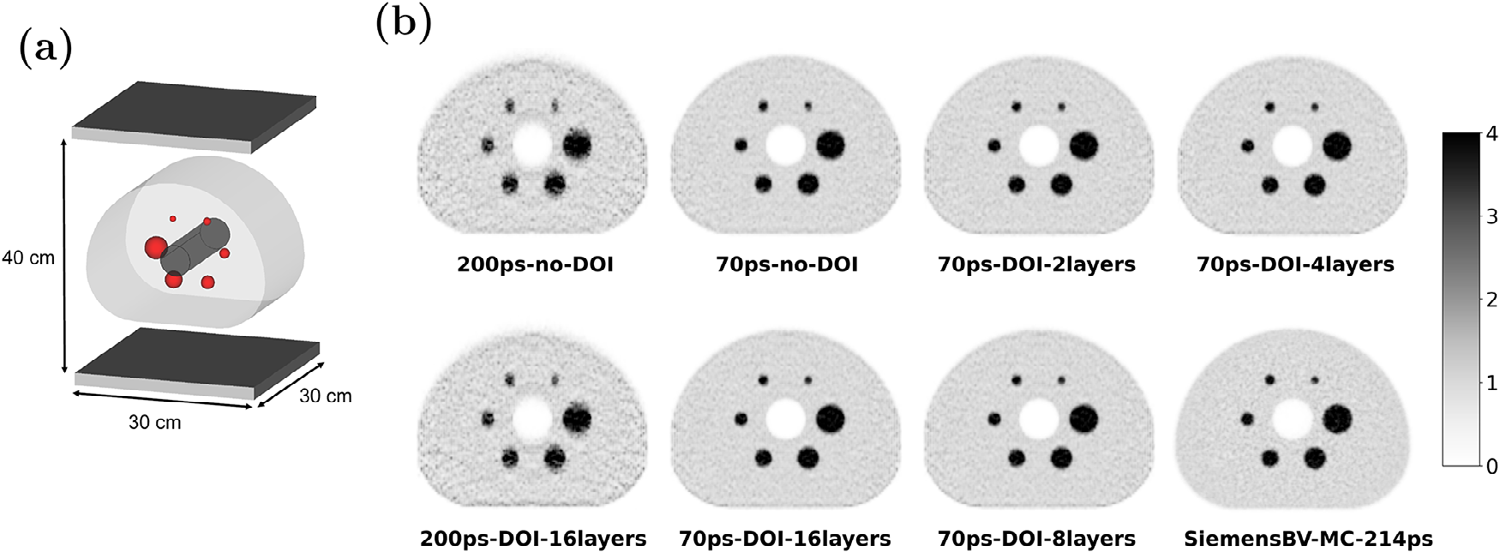
\includegraphics[width=0.9\linewidth]{img/razdevsek2025-nema.png}
\end{center}

\paragraph{Why it matters here}
Not monolithic, but it answers a question a monolithic panel has to: how good
does DOI need to be? In a panel at \ps{70}, \mm{2.5} FWHM is enough and more is
wasted --- a target a thick monolith can be measured against, set by an
image-level study rather than by detector pride. But it is the saturation
point of an ideal detector with \mm{3} pixels: no decoding error, no
depth-dependent timing, scatter merged to a centroid. A monolith with finer
transverse resolution may keep gaining past \mm{2.5}, and its real DOI error
and scatter tails are what this study leaves out. It is also the high-timing
end of the panel argument whose monolithic end is \ref{prog:WTPET}
(\ps{300}, \mm{2.67} DOI): the two together bracket what a monolithic panel's
timing and DOI buy in an image.

\end{papernote}

\end{programnote}

\begin{programnote}{Seoul SNU -- Jae Sung Lee group, inter-crystal scatter recovery}{Seoul}
\location[-202,144]{37.46}{126.95}{Seoul, South Korea}

\paragraph{What it is}
Jae Sung Lee's group in Nuclear Medicine at Seoul National University (with the
spin-off Brightonix Imaging): light-sharing PET detectors and learned decoding,
here for events that scatter between crystals.

\paragraph{People}
Jae Sung Lee; Seungeun Lee --- by name and topic very likely the Seungeun Lee
now at \ref{prog:LBNL}, first author of \ref{note:Lee2026}.

\begin{papernote}{Lee and Lee 2021 -- Inter-crystal scattering recovery of light-sharing PET detectors using convolutional neural networks}{Lee2021}
\thumb{img/lee2021.png}
Phys.\ Med.\ Biol.\ 66(18):185004, \doi{10.1088/1361-6560/ac215d}.

\paragraph{Summary}
Simulation (GATE with optical transport) of four \mm{20} LSO arrays on one
8 x 8 SiPM array through a glass window: pitches 3.2, 2.1, 1.6 and \mm{1.2},
so crystal-to-sensor ratios from 1:1 to 2.6:1. Two CNNs on the 8 x 8 map:
one regresses the energy in every crystal and then picks the event's one or two
crystals, the other classifies the first-interacted crystal directly. Within a
crystal, multiple hits are summed; only the two main crystals are recovered,
so the 5--10\% of events in three or more crystals are treated as two-crystal
ones. No timing.

\paragraph{Key Findings}
\begin{itemize}
	\item Inter-crystal scatter grows as crystals shrink: two-crystal events
		28.6\% at \mm{3.2} pitch, 33.5\% at \mm{1.2}; photoelectric
		66.3 to 56.5\%.
	\item The energy network separates events correctly 97, 92, 90 and 77\%
		of the time and picks the right crystal pair 91, 78, 62 and 35\%,
		roughly matching a constrained-optimisation baseline at coarse pitch
		and beating it at fine.
	\item The classifier finds the first crystal about twice as often as no
		recovery for scattered events.
	\item In a simulated ring, centre radial FWHM \mm{1.88} to \mm{1.69}
		(\mm{3.2} pitch) and \mm{0.94} to \mm{0.73} (\mm{1.2}); off centre,
		parallax dominates.
\end{itemize}

\paragraph{Why it matters here}
The learned version of the decomposition \ref{note:Petersen2020} does with
fixed patterns, on ordinary light sharing --- and it degrades exactly as the
patterns overlap, 91\% to 35\% for the crystal pair. It never orders, and
cannot be trained on measured data, since true per-crystal energies are
unknown; the authors suggest transfer from simulation.
\end{papernote}

\end{programnote}

\begin{programnote}{IFIC Valencia -- Rafecas group and the AX-PET collaboration}{AXPET}
\location[-487,627]{39.51}{-0.42}{Paterna, Valencia, Spain}

\paragraph{What it is}
Magdalena Rafecas's image-reconstruction group at IFIC (CSIC--University of
Valencia), working with CERN and ETH on AX-PET, a demonstrator with long axial
LYSO crystals and orthogonal wavelength-shifting strips: crystal layers for
depth, strips for the axial coordinate.

\paragraph{People}
John Gillam (later University of Sydney), Paola Solevi, Josep Oliver, Magdalena
Rafecas (IFIC, later Lübeck); Christian Joram, Matthieu Heller (CERN); Chiara
Casella (ETH Zurich).

\begin{papernote}{Gillam et al.\ 2014 -- Sensitivity recovery for the AX-PET prototype using inter-crystal scattering events}{Gillam2014}
\thumb{img/gillam2014.png}
Phys.\ Med.\ Biol.\ 59(15):4065--4083, \doi{10.1088/0031-9155/59/15/4065}.

\paragraph{Summary}
Two heads of six layers of eight \qtyproduct{3 x 3 x 100}{\mm} axial LYSO
crystals interleaved with WLS strips, all on SiPMs; energy resolution 11.8\%
for one crystal. Inter-crystal scatter enters as ``triples'': three resolved
hits, two in one head, which give two candidate lines of response. Four ways
to use them in list-mode MLEM: as two separate events, by selecting one (by the
Klein--Nishina cross-section or at random), or by inclusion --- one system-matrix
row that is the half-and-half sum of both candidates, a ``V-projection''. The
interaction order is deliberately not determined. Measured data, NEMA NU 4
phantom and rats.

\paragraph{Key Findings}
\begin{itemize}
	\item Triples are about 22\% of the data.
	\item Klein--Nishina selection was no better than random.
	\item Only inclusion improved every figure of merit: SNR 12.7 to 13.3,
		spill-over 89.8 to 82.9 (\num{e-3}), resolution unchanged; with 90\%
		of the data it matched the full data without triples. A 5--10\% gain,
		less than 20\% more clean events would give, because a V-projection is
		about twice as long as a line.
	\item The literature it cites puts first-interaction identification below
		70\%.
\end{itemize}

\paragraph{Why it matters here}
The reconstruction-side answer to multi-interaction events: if the order
cannot be told, carry both candidates and let the reconstruction weigh them.
It sets the bar from the other end --- an ordering method is only worth having
if it beats simply including both lines.
\end{papernote}

\end{programnote}

% ===========================================================================
% Clinical scanners: the commercial systems the detectors on this map would
% have to displace. A reference, not a research line; the leaderboard's
% clinical rows are read from the papers here. Fixed under the detector radar by
% [map] fixed in notesmap.toml: a Bern pin sits in the fan of Geneva leaders.
% ===========================================================================

\begin{programnote}{Clinical scanners -- the commercial yardstick}{Clinical}

\paragraph{What it is}
The clinical systems a monolithic or DOI detector has to beat, kept as a
reference rather than a research line: four NEMA NU 2 evaluations chosen to
span the field. Siemens Healthineers' Biograph Vision 600 and its long-axial
Quadra share one LSO detector, the best timing of the four; United
Imaging's uEXPLORER has the finest pitch of the four and the longest field; GE
HealthCare's Omni Legend is BGO without TOF. All are pixelated, read out at
one end, and have no DOI; together they are the \ref{prog:Leaderboard}'s
clinical reference band.
\gap{Philips (Vereos, Vereos Z) is the one major vendor not here; and none of
these papers measures DOI or parallax, which is the axis the map's detectors
compete on.}

\paragraph{Why it matters here}
The detector figures that a new architecture is compared against, from NEMA
measurements rather than datasheets. Transverse resolution is set by the pitch
(2.8--\mm{4.1}) and the depth error by the whole crystal (18--\mm{30}), so the
room a monolith has to win is mostly in depth. On timing the clinical range is
wide: \ps{210} on the Vision is matched on this map only by
\ref{note:Carra2022} (\ps{156}), \ref{note:Pizzichemi2019} (\ps{157}, light
sharing) and \ref{note:Borghi2016} (\ps{214}), while \ps{505} on the
uEXPLORER is beaten by most of them, and the Omni Legend has no TOF at all.

\begin{papernote}{Prenosil et al.\ 2022 -- Performance characteristics of the Biograph Vision Quadra PET/CT system with a long axial field of view using the NEMA NU 2-2018 standard}{Prenosil2022}
\thumb{img/prenosil2022.png}
J.\ Nucl.\ Med.\ 63(3):476--484 (2022; online 2021),
\doi{10.2967/jnumed.121.261972}. Prenosil, Sari, Fürstner, Afshar-Oromieh,
Shi, Rominger, Hentschel --- Bern University Hospital with Siemens Healthcare.

\paragraph{Detector}
The Biograph Vision 600's detector, four times over: \qtyproduct{3.2 x 3.2 x
20}{\mm} LSO crystals, 5 x 5 on a \qtyproduct{16 x 16}{\mm} SiPM array (a
mini block), eight mini blocks to a block, 38 blocks to a ring and 32 rings ---
\cm{106} axial, 320 crystals long. Data are taken with every ring pair (MRD
322); the clinical software reconstructs with ring differences up to 85.

\paragraph{Key Findings}
\begin{itemize}
	\item Spatial resolution, NEMA NU 2-2018: 3.3/3.4/\mm{3.8} FWHM radial,
		tangential, axial --- the pitch shows through.
	\item Sensitivity 83 cps/kBq at MRD 85 and 176 cps/kBq at MRD 322;
		peak NECR 1613 and 2956 kcps, both at 27.49 kBq/mL, scatter fraction
		36\% and 37\%.
	\item TOF \ps{225} at low activity, \ps{228} at peak NECR (MRD 85);
		energy resolution 9.8\% at low activity, 10.1\% at peak NECR, 8.9\%
		with a \textsuperscript{68}Ge source and no scatter.
	\item Contrast recovery 70--87\% at 4:1 and 75--93\% at 8:1 with PSF-TOF (Table 6; the abstract says 77.7\%);
		30-second frames still gave readable clinical images.
\end{itemize}

\paragraph{Why it matters here}
The source of the leaderboard's Quadra row: transverse \mm{3.2} (the pitch),
energy 9.8\%, CTR \ps{225}. It reports no DOI because the detector has none;
the \mm{12.6} the row carries is modelled from the crystal, not measured
here. The sensitivity is what a long axial field buys, not the detector, so
it sits in no detector table.
\end{papernote}

\begin{papernote}{van Sluis et al.\ 2019 -- Performance characteristics of the digital Biograph Vision PET/CT system}{vanSluis2019}
\thumb{img/vansluis2019.png}
J.\ Nucl.\ Med.\ 60(7):1031--1036, \doi{10.2967/jnumed.118.215418}. van Sluis,
de Jong, Schaar, Noordzij, van Snick, Dierckx, Borra, Willemsen, Boellaard ---
University Medical Center Groningen.

\paragraph{Detector}
The Quadra's detector at standard length: \qtyproduct{3.2 x 3.2 x 20}{\mm} LSO
in 5 x 5 mini blocks on \qtyproduct{16 x 16}{\mm} SiPM arrays, the crystal face
fully covered by silicon, eight rings of 38 blocks, \cm{26.1} axial, \cm{78}
bore. Measured to NEMA NU 2-2012, with the 2018 additions, against the
photomultiplier Biograph mCT Flow it replaced.

\paragraph{Key Findings}
\begin{itemize}
	\item Spatial resolution 3.6/\mm{3.5} transverse/axial FWHM at \cm{1}.
	\item Sensitivity 16.4 kcps/MBq; peak NECR 306 kcps at 32.6 kBq/mL,
		scatter fraction 38.7\%.
	\item TOF \ps{210}, \ps{215} by peak NECR --- against \ps{540} on the mCT
		Flow.
	\item No energy resolution reported.
\end{itemize}

\paragraph{Why it matters here}
The same detector as \ref{note:Prenosil2022} on a short ring, so the pair
separates what the detector gives from what axial length buys: a tenth of the
sensitivity, the same timing. \ps{210} against \ps{540} is the size of the step
SiPMs with full coverage made, the step a monolith's timing is measured
against.
\end{papernote}

\begin{papernote}{Spencer et al.\ 2021 -- Performance evaluation of the uEXPLORER total-body PET/CT scanner based on NEMA NU 2-2018}{Spencer2021}
\thumb{img/spencer2021.png}
J.\ Nucl.\ Med.\ 62(6):861--870, \doi{10.2967/jnumed.120.250597}. Spencer,
Berg, Schmall, Omidvari, Leung, Abdelhafez, Tang, Deng, Dong, Lv, Bao, Liu, Li,
Jones, Badawi, Cherry --- UC Davis with United Imaging Healthcare.

\paragraph{Detector}
Eight PET units, \cm{194} axial and \cm{78.6} across. Blocks of 7 x 6
\qtyproduct{2.76 x 2.76 x 18.1}{\mm} LYSO crystals read by four
\qtyproduct{6 x 6}{\mm} SiPMs through a light guide (Anger multiplexing,
10.5:1) --- 564\,480 crystals on 53\,760 channels. Transaxially adjacent
blocks within a module share energy (axial ones do not), so a photon that Compton-scatters out of an edge crystal
is recovered rather than lost. Window 430--\keV{645}.

\paragraph{Key Findings}
\begin{itemize}
	\item Sensitivity 174 kcps/MBq at the centre; peak NECR 1524 kcps at 17.3
		kBq/mL (36.3\% scatter), 1855 kcps with a \cm{175} phantom.
	\item Spatial resolution about \mm{3.0} FWHM near the centre (FBP).
	\item TOF \ps{505} system-wide, \ps{412} averaged over individual lines of
		response --- the gap the authors put down to an incomplete TOF
		calibration across half a million crystals.
	\item No energy resolution reported.
\end{itemize}
\aside{The detector is not the uEXPLORER's selling point: finer crystals than
the Vision's, reached by sharing light, at more than twice its CTR. It wins on
length. The inter-block scatter recovery is a clinical scanner keeping
inter-crystal scatter events, the ones Prism-PET discards.}

\paragraph{Why it matters here}
The opposite corner from the Vision: the finest pitch of these four and the
longest field of any clinical scanner, with timing a monolithic build already beats. And a
calibration problem a monolith would make larger: TOF across 564\,480 crystals
is not yet calibrated, and a monolith calibrates positions as well.
\end{papernote}

\begin{papernote}{Yamagishi et al.\ 2023 -- Performance characteristics of a new-generation digital BGO PET/CT system, Omni Legend 32, according to NEMA NU 2-2018}{Yamagishi2023}
\thumb{img/yamagishi2023.png}
J.\ Nucl.\ Med.\ 64(12):1990--1997, \doi{10.2967/jnumed.123.266140}.
Yamagishi, Miwa, Kamitaki, Anraku, Sato, Yamao, Kubo, Miyaji, Oguchi ---
Aizawa Hospital and Fukushima Medical University.

\paragraph{Detector}
GE HealthCare's digital BGO system: \qtyproduct{4.1 x 4.1 x 30}{\mm} BGO, 72
crystals on 18 \qtyproduct{6 x 6}{\mm} SiPMs per block, 22 modules,
\cm{32} axial, \mm{725} ring. Window 435--\keV{580}. No TOF; a network
trained on TOF images (Precision DL) stands in for it.

\paragraph{Key Findings}
\begin{itemize}
	\item Spatial resolution 4.3/5.3/\mm{6.2} at 1/10/\cm{20} (FBP),
		3.7/4.3/\mm{5.1} with OSEM.
	\item Sensitivity 47.3 cps/kBq; peak NECR 501.7 kcps at 15.7 kBq/mL,
		scatter fraction 35.4\%.
	\item Energy resolution 9.8\%, stated in the discussion, not measured
		in the paper.
\end{itemize}

\paragraph{Why it matters here}
BGO back in a clinical scanner, chosen for stopping power and cost at the price
of timing: three times the Vision's sensitivity at a similar length, from
\mm{30} of the densest common scintillator. It is the market's answer to the
question \ref{note:Cates2024} and the BGO semi-monoliths ask, and the
comparator a BGO monolith has to beat: \mm{30} with no DOI is the worst
parallax of any detector here (17 mm modelled).
\end{papernote}

\end{programnote}

% ===========================================================================
% Leaderboard: measured detector builds on this map, side by side. Placed to
% the right of the map by [map] fixed in notesmap.toml, and open by default.
% Keep it to measurements; simulations and MAE-only figures stay out.
% ===========================================================================

\begin{programnote}{Leaderboard -- measured detector builds, ranked by DOI against thickness}{Leaderboard}

\paragraph{What it is}
Every detector build on this map with a figure for depth of interaction,
ranked by DOI as a share of crystal depth (DOI/d), with simulated detectors,
clinical scanners and scanner-level counts in separate tables. Every cell is a
number; a letter after it says what kind: unmarked is a measured FWHM, and
\begin{itemize}
	\item p --- the crystal pitch, where the build resolves crystals rather than
		positions;
	\item L, b --- the layer or bin width, for builds that resolve depth in
		steps (a uniform step of width $w$ is Gaussian-equivalent to $0.68\,w$);
	\item f --- fitted from flood data, with no collimated beam;
	\item e --- a Gaussian equivalent the authors computed;
	\item r --- a CTR against a reference crystal, not between two such
		detectors;
	\item i --- an input to a simulation, not a result;
	\item m --- modelled here, not reported.
\end{itemize}
A dash is not reported. Builds quoting only a mean absolute error (Zhang 2017,
Thull 2026) are left out.

\paragraph{Measured builds}
Builds that resolve depth continuously first, then those that resolve it in
steps.

\begin{center}
\begin{scriptsize}
\setlength{\tabcolsep}{1.5pt}
\begin{tabular}{lllllllll}
\hline
Build & Detector & Readout & Depth mm & DOI mm & DOI/d \% & Trans. mm & Energy \% & CTR ps \\
\hline
Xie 2026 & LYSO 0.44 mm pixels & dual & 20 & 1.78 & 9 & 0.5 p & 22.7 & 1152 \\
LaBella 2021 & LYSO 1.4 mm, Prism + CNN & single & 20 & 1.84 & 9 & 1.6 p & 8.7 & -- \\
Ren 2014 & LSO 1.5 mm, unpolished & dual & 20 & 1.9 & 10 & 1.5 p & 22 & -- \\
Kuang 2020 & LYSO 1 mm pixels, aPET & dual & 20 & 1.96 & 10 & 1.07 p & 19.1 & 1200 r \\
Enríquez 2026 & LYSO 0.785 mm, panel & dual & 20 & 2.0 & 10 & 0.85 p & 15.6 & -- \\
Enríquez 2025 & LYSO 0.785 mm, 9:1 mux & dual & 20 & 2.3 & 12 & 0.85 p & 10.5 & 1300 \\
Zeng 2024 & LYSO 1.5 mm, tapered Prism & single & 20 & 2.52 & 13 & 1.6 p & 8.9 & 243 \\
LaBella 2020 & LYSO 1.4 mm, Prism & single & 20 & 2.5 & 13 & 1.6 p & 9 & -- \\
Zhang 2021 & LYSO 1.37 mm slabs & dual & 20 & 2.60 & 13 & 1.97 & 21.7 & 718 r \\
Zeng 2023 & LYSO 1.5 mm, Prism scanner & single & 20 & 2.85 & 14 & 1.22 & 12.6 & 271 \\
Zhang 2019 & LYSO 1 mm slabs, painted & single & 10 & 1.55 & 16 & 1.07 & 24.9 & 788 r \\
Gsell 2020 & LYSO monolith, 50 mm & single & 10 & 1.6 f & 16 & -- & 16.6 & -- \\
Kinyanjui 2025 & LYSO 0.96 mm slabs, XGBoost & single & 10 & 1.67 & 17 & 0.92 & -- & -- \\
Borghi 2016 & LYSO monolith, 32 mm & single & 22 & 3.73 & 17 & 1.68 & 9.9 & 214 \\
Freire 2022 & LYSO annulus & single & 10 & 1.8 f & 18 & -- & 23.4 & -- \\
Carra 2022 & LYSO monolith & single & 8 & 1.55 & 19 & 0.78 & 11 & 156 \\
Pizzichemi 2019 & LYSO 1.53 mm, sharing & single & 15 & 3 & 20 & 1.6 p & 8.9 & 157 \\
Kinyanjui 2026 & LYSO 0.96 mm slabs, painted & single & 10 & 2.14 & 21 & 1.68 & 17.4 & 3340 r \\
Kuang 2026 & GAGG 0.96 mm slabs & single & 10 & 2.33 & 23 & 1.60 & 15.6 & 4300 r \\
Zhang 2021 & LYSO 1.37 mm slabs & single & 20 & 4.77 & 24 & 2.43 & 25.7 & 779 r \\
Li 2012 & LYSO monolith, cMiCE & single & 15 & 3.69 & 25 & 1.55 & -- & -- \\
Cucarella 2026 & LYSO 0.97 mm slabs, 25.6 mm & single & 12 & 3.08 & 26 & 1.7 & 16.4 & 252 \\
Pizzichemi 2016 & LYSO 1.53 mm, sharing & single & 15 & 4.1 & 27 & 1.6 p & 12.7 & 353 \\
Freire 2026 & LYSO curved monolith & single & 12.5 & 3.6 & 29 & -- & 19 & -- \\
Moliner 2012 & LYSO monolith, MAMMI & single & 10 & 4 & 40 & 1.6 & 18 & -- \\
\hline
Yamaya 2011 & LYSO 1 mm cubes, X'tal cube & 6 faces & 16 & 1 L & 6 & 1 p & 12.7 & -- \\
Stockhoff 2021 & LYSO monolith, 50 mm & single & 16 & 2.67 L & 17 & 1.14 & 11.0 & -- \\
Gillam 2014 & LYSO 3 mm axial, 6 layers & SiPM & 18 & 3 L & 17 & 3 p & 11.8 & -- \\
Krishnamoorthy 2018 & LYSO monolith, β-CUBE & single & 8 & 1.6 L & 20 & 0.78 & 12 & -- \\
Peng 2019a & LYSO monolith, 4 stacked layers & 4 sides & 13.4 & 3.36 L & 25 & 1.1 & 10.3 & 348 r \\
Lee 2026 & BGO semi-monolith & single & 20 & 5 b & 25 & 3.17 & 21 & 172 r \\
Kang 2023 & LYSO 0.9 mm, 3 layers & SiPM & 15 & 5 L & 33 & 1 p & 24.3 & 9500 \\
Cates 2024 & BGO monolith & single & 15 & -- & -- & -- & 17.6 & 315 \\
Xu 2019 & LYSO ring monolith & 2 rings & 5 & -- & -- & 1.44 & 10.7 & -- \\
\hline
\end{tabular}
\end{scriptsize}
\end{center}

\paragraph{Simulated detectors}
Not builds: simulation results, on the same columns and the same ranking, kept
apart so they are never read as measurements. Most model no electronics, ideal
or near-ideal photodetection, and often no noise; where a column is an input
rather than a result it is marked i.

\begin{center}
\begin{scriptsize}
\setlength{\tabcolsep}{1.5pt}
\begin{tabular}{lllllllll}
\hline
Build & Detector & Readout & Depth mm & DOI mm & DOI/d \% & Trans. mm & Energy \% & CTR ps \\
\hline
Decuyper 2021 & LYSO monolith, unscattered & single & 16 & 0.71 & 4 & 0.42 & -- & -- \\
Razdevšek 2025 & LSO 3 mm pixels, 8 layers & ideal & 20 & 1.7 e & 9 & 3 p & 10 i & 70 i \\
Li 2012 & LYSO monolith, cMiCE SES & entrance & 15 & 1.52 & 10 & 0.91 & -- & -- \\
Decuyper 2021 & LYSO monolith, scattered & single & 16 & 1.80 & 11 & 0.66 & -- & -- \\
Petersen 2020 & LYSO 1.4 mm, Prism, ICS & single & 20 & 2.1 & 11 & 1.4 p & 10 i & -- \\
Petersen 2024 & LYSO 1.4 mm, Prism, photopeak & single & 20 & 3.0 & 15 & 1.4 p & -- & -- \\
Peng 2019 & LYSO monolith, 4 stacked layers & 4 sides & 13.4 & 3.36 L & 25 & 0.40 & 9.3 & -- \\
\hline
\end{tabular}
\end{scriptsize}
\end{center}

Decuyper's first row is unscattered events only (0.42 transverse is its
non-Compton FWHM); its scattered events, about 60\% of the total, follow
further down. Razdevšek's DOI is the 2.5 mm layer as a Gaussian-equivalent
FWHM; Petersen's is the multi-crystal events of a CNN, 1.0 mm for
single-crystal ones, and its 10\% energy resolution is set from experiment.
Petersen 2024's DOI is for every photopeak event, \mm{2.4} for photoelectric
ones and \mm{4.2} for inter-crystal scatter.
Decuyper's DOI for all events is \mm{0.99}, transverse \mm{0.46}. Peng 2019
is the simulation of the layered block measured as Peng 2019a above; its depth
is the \mm{3.36} layer pitch, reflector included.

\paragraph{Clinical reference}
What the detectors above are measured against: the detectors of four current
clinical scanners (\ref{prog:Clinical}), from their NEMA NU 2 evaluations ---
energy resolution at low count rate where reported, and TOF. None has DOI, so
none reports a DOI resolution; the figure is modelled here (marked m) as the
Gaussian-equivalent FWHM of the depth at which 511 keV photons interact in the
crystal, the depth error of a detector that assigns every event one depth.
For \mm{20} of LSO ($\mu \approx \qty{0.087}{\per\mm}$) that is \mm{12.6},
63\% of the crystal; the whole-depth bin would be \mm{20} and a uniform spread
\mm{13.6}. LYSO is taken at \qty{0.083}{\per\mm} and BGO at
\qty{0.095}{\per\mm}. The Omni Legend's energy resolution is stated in its
paper, not measured there, and it has no TOF; van Sluis and Spencer report no
energy resolution.

\begin{center}
\begin{scriptsize}
\setlength{\tabcolsep}{1.5pt}
\begin{tabular}{lllllllll}
\hline
Build & Detector & Readout & Depth mm & DOI mm & DOI/d \% & Trans. mm & Energy \% & CTR ps \\
\hline
Prenosil 2022 & LSO 3.2 mm, Vision Quadra & single & 20 & 12.6 m & 63 & 3.2 p & 9.8 & 225 \\
van Sluis 2019 & LSO 3.2 mm, Vision 600 & single & 20 & 12.6 m & 63 & 3.2 p & -- & 210 \\
Spencer 2021 & LYSO 2.76 mm, uEXPLORER & single & 18.1 & 11.6 m & 64 & 2.76 p & -- & 505 \\
Yamagishi 2023 & BGO 4.1 mm, Omni Legend & single & 30 & 17.0 m & 57 & 4.1 p & 9.8 & -- \\
\hline
\end{tabular}
\end{scriptsize}
\end{center}

\paragraph{Scanners}
The systems on this map built from such detectors, with what a detector table
cannot show: how many counts a scanner keeps. Peak sensitivity is the absolute
NEMA figure at the centre, in percent (1\% is \qty{10}{cps/\kilo\becquerel}), and
it moves with bore, axial length and energy window as much as with the crystal,
so read it beside them. NECR is the peak noise-equivalent count rate and the
activity it peaks at, for the phantom named.

\begin{center}
\begin{scriptsize}
\setlength{\tabcolsep}{2pt}
\begin{tabular}{llllllll}
\hline
Build & Detector & Bore mm & Axial mm & Sens. \% & Window keV & NECR kcps & at MBq \\
\hline
Kuang 2020 & LYSO 1 mm pixels, dual-ended & 111 & 105.6 & 16.0 & 250--750 & 324 & 26.4 \\
Krishnamoorthy 2018 & LYSO monolith, 8 mm & 76 & 130 & 12.4 & 255--765 & 300 & 33 \\
Gsell 2020 & LYSO monolith, 10 mm & 114 & 150 & 11.0 & not stated & 486 & 23 \\
Kang 2023 & LYSO 0.9 mm, 3 layers & 52.5 & 51.5 & 8.66 & 250--750 & 46.9 & -- \\
Pajak 2016 & LYSO monolith, 10 mm & 111 & 94.4 & 5.3 & 255--767 & 72 & 7.1 \\
Freire 2022 & LYSO annulus & 62 & 25.8 & 3.8 & 50\% & 40.6 & 10.0 \\
Cucarella 2026 & LYSO 0.97 mm slabs, 12 mm & 106 & 52 & 3.5 & 358--664 & 106.9 & 11.7 \\
Freire 2026 & LYSO curved monolith ring & 200 & 50 & 2.0 & 408--613 & 15 & 13.4 \\
Moliner 2012 & LYSO monolith, MAMMI & 186 & 40 & 1.8 & 250--750 & 25 & 44 \\
Zeng 2023 & LYSO 1.5 mm, Prism & 385 & 25.5 & 1.2 & 400--650 & -- & -- \\
\hline
\end{tabular}
\end{scriptsize}
\end{center}
NECR is for the mouse phantom except Freire 2026 (rat) and Moliner 2012 (a
\qtyproduct{60 x 170}{\mm} breast-scaled phantom). Bore is the detector ring
diameter where the paper gives no aperture (Kuang 2020, Krishnamoorthy 2018,
Pajak 2016, whose aperture is \mm{105}). Window is the sensitivity window; Kuang
2020's NECR is at 350--\keV{750} and Krishnamoorthy's at the default $\pm$15\%.
Freire 2022's window is given only as 50\%. Kang 2023's sensitivity
falls to 2.84\% at 400--\keV{600} once inter-crystal scatter is windowed out;
Kuang 2020's to 11.9\% at 350--\keV{750}; Pajak's to 4.2\% at 358--\keV{664}.
Krishnamoorthy's NECR is the paper's 300 kcps at about \MBq{33}. Zeng 2023's
ring is a decagon, \mm{385} by \mm{291}; the long diameter is given.

\paragraph{Clinical scanners}
The same counts for the clinical reference, with the NEMA NU 2 body phantom in
place of the mouse: NECR peaks at an activity concentration, not an activity.
Ring is the detector diameter face to face. Sensitivity is the line-source
figure at the centre, in the same percent as above; the Quadra's is with every
ring pair (MRD 322), 8.3\% as reconstructed clinically (MRD 85).

\begin{center}
\begin{scriptsize}
\setlength{\tabcolsep}{2pt}
\begin{tabular}{llllllll}
\hline
Build & Detector & Ring mm & Axial mm & Sens. \% & Window keV & NECR kcps & at kBq/mL \\
\hline
Prenosil 2022 & LSO 3.2 mm, Vision Quadra & 820 & 1060 & 17.6 & 435--585 & 2956 & 27.5 \\
Spencer 2021 & LYSO 2.76 mm, uEXPLORER & 786 & 1940 & 17.4 & 430--645 & 1524 & 17.3 \\
Yamagishi 2023 & BGO 4.1 mm, Omni Legend & 725 & 320 & 4.73 & 435--580 & 501.7 & 15.7 \\
van Sluis 2019 & LSO 3.2 mm, Vision 600 & -- & 261 & 1.64 & -- & 306 & 32.6 \\
\hline
\end{tabular}
\end{scriptsize}
\end{center}
The Vision 600 paper gives a \mm{780} bore rather than the ring.

\paragraph{Notes on the rows}
Pizzichemi 2019's \mm{3} DOI is cited from earlier work, Freire 2026's figures
are partly system-level, Xu 2019's transverse is the angle FWHM before its
authors' half-difference correction (\mm{0.94} after) and it has no depth at all, Freire 2026 has no TOF, Stockhoff never states its six layers' thickness (\mm{2.67} is
16/6, as the later WT-PET papers take it), and Kang 2023's \ns{9.5} is the
whole system's timing resolution, an order of magnitude outside TOF; its
three layers are 4, 4 and \mm{7}, so \mm{5} is their mean. Krishnamoorthy 2018's ($\beta$-CUBE) depth is five
layers in \mm{8} (its \mm{1.6} is the layer width), its \mm{0.78} transverse
is the paper's average over the central 80\% of the block (\mm{0.9} over all of
it; the vendor abstract, \ref{note:Mollet2017}, gives \mm{0.76}), and it reports
a \ns{5} coincidence window but no CTR.
Zeng 2023's \ps{271} needs an extra LOR-based fine-tuning; its images use \ps{330}.
Zeng 2024's DOI is the module average (\mm{2.25} in a centre crystal). Lee
2026's four depth bins hold equal counts, not equal widths; \mm{5} is the
authors' nominal width.
Prism-PET's transverse is the \mm{1.6} pitch: \mm{1.4} crystals with
\mm{0.2} of BaSO$_4$ between them, or \mm{1.5} with \mm{0.1} in Zeng 2024; LaBella 2021's 8.7\% energy is read off its
Fig.\ 2, and LaBella 2020's 9\% is after DOI correction (14\% before). Ren
2014's 22\% is the geometric-mean energy (30\% summed). Moliner 2012's detector
figures and Gillam 2014's energy are cited from earlier papers, not measured
there. Cates 2024's \ps{315} is the authors' estimate between two such
detectors for the fast, Cherenkov-carrying half of its events (\ps{237}
measured against an LYSO reference), unflagged like Carra's and Borghi's
reference-corrected figures. No CTR is reported for any row left blank: those papers give a
coincidence window or nothing.

\end{programnote}

% ===========================================================================
% Design fit: which detector architecture suits which clinical use. Ratings are
% first-principles judgements on eight system-level axes, editable here; the
% board draws them as a radar with a fit score per pair (tables.DesignFit).
% ===========================================================================

\begin{programnote}{Design fit -- what each application asks of a scanner, and what each detector gives}{DesignFit}

\paragraph{What it is}
Three tiers: detectors estimate position, depth, energy and time; scanners
turn those into system metrics; clinical uses each lean on some system metrics
more than others. These two tables rate both sides on the same eight system
axes, 1 (barely matters, or weak) to 5 (dominant, or strong), so a detector's
weaknesses can be checked against what a use can tolerate. The ratings are
first-principles judgements, not measurements; change them here and the board
follows.

\paragraph{Application demand}

\begin{center}
\begin{scriptsize}
\setlength{\tabcolsep}{2.5pt}
\begin{tabular}{lllllllll}
\hline
Application & Resolution & DOI uniformity & Sensitivity & TOF & Count rate & Quantitation & Axial reach & Energy \\
\hline
Small-lesion oncology & 5 & 3 & 4 & 4 & 2 & 3 & 2 & 3 \\
Quantitative response & 3 & 3 & 3 & 3 & 2 & 5 & 2 & 4 \\
Low dose, paediatric & 3 & 2 & 5 & 5 & 1 & 3 & 4 & 3 \\
Dynamic, total-body & 2 & 2 & 5 & 4 & 5 & 4 & 5 & 3 \\
Brain & 5 & 5 & 3 & 3 & 2 & 4 & 2 & 3 \\
Cardiac & 3 & 2 & 4 & 4 & 4 & 4 & 2 & 3 \\
RT and surgical planning & 4 & 4 & 2 & 3 & 1 & 4 & 2 & 3 \\
Theranostics (Y-90) & 3 & 2 & 5 & 4 & 1 & 4 & 3 & 5 \\
\hline
\end{tabular}
\end{scriptsize}
\end{center}

\paragraph{Architecture supply}

\begin{center}
\begin{scriptsize}
\setlength{\tabcolsep}{2.5pt}
\begin{tabular}{lllllllll}
\hline
Architecture & Resolution & DOI uniformity & Sensitivity & TOF & Count rate & Quantitation & Axial reach & Energy \\
\hline
Pixelated, no DOI & 2 & 1 & 4 & 5 & 5 & 4 & 5 & 4 \\
Prism-PET & 3 & 4 & 3 & 4 & 4 & 4 & 3 & 5 \\
Dual-ended pixelated & 4 & 5 & 3 & 2 & 4 & 4 & 2 & 3 \\
Semi-monolithic slabs & 4 & 4 & 4 & 3 & 3 & 3 & 4 & 3 \\
Thin monolith & 5 & 4 & 2 & 4 & 3 & 3 & 3 & 3 \\
Thick monolith & 4 & 3 & 5 & 3 & 2 & 3 & 3 & 3 \\
\hline
\end{tabular}
\end{scriptsize}
\end{center}

\paragraph{Reading it}
The fit of a detector to a use weights each axis by how much the use cares,
\[ \mathrm{fit} = \frac{\sum_i d_i \min(s_i, d_i)}{\sum_i d_i^2}, \]
where $d$ is demand and $s$ supply, so 100\% means no axis falls short and a shortfall costs most where the
demand is highest. The supply ratings are judgements informed by the leaderboard, not read off
it: pixelated
blocks without DOI are the clinical baseline, fast and cheap to scale but
blind to depth; Prism-PET buys DOI and energy resolution with the scatter it
rejects; dual-ended readout has among the best DOI, with poor timing and higher cost;
monoliths keep the scattered counts and position continuously, but their
timing and positioning depend on modelling the spread light, and they need
calibration that quantification must trust. A thick monolith that recovered its
multi-interaction events and its timing would move its supply polygon
outward on exactly the axes where it falls short --- which is the thesis.

\end{programnote}

% ===========================================================================
% Experiment ideas: papers and simulations this map suggests, each with the
% numbers it has to beat and the notes they come from. Cards are ideas, not
% papers, so their keys start with Idea and they carry no year.
% ===========================================================================

\begin{programnote}{Experiment ideas -- simulations, benchmarks and papers this map suggests}{Ideas}
\location[109,-702]{-33.88}{151.20}{Sydney, Australia}

\paragraph{What it is}
Studies the literature on this map points to and leaves undone, each pinned to
the published numbers it would have to beat and the papers they come from.
Most share one setup: a GATE optical simulation of a thick LYSO monolith or
semi-monolith with per-channel photon counts and arrival times recorded, so
that one dataset serves several cards.

\begin{papernote}{Idea -- order two-site events from photon arrival times}{IdeaOrdering}
\paragraph{The idea}
For events that deposit in two places, estimate which came first from the
joint pattern of per-channel arrival times and counts, in a continuous crystal.

\paragraph{To beat}
Energy-only layer sequencing, 69.2\% by closest layer and 81.3\% with the
backscatter swap for two-layer events (\ref{note:Peng2019}); the experiment
gave up sequencing for a max-energy rule (\ref{note:Peng2019a}). First crystal
recovered for 88\% of multi-crystal events by a CNN on the readout pattern, in
simulation; the analytical decomposition only finds which crystals fired (99\%)
(\ref{note:Petersen2020}); the journal version picks the first crystal of
64.7\% of inter-crystal-scatter events and 83\% of the photopeak, still
simulated (\ref{note:Petersen2024}). Both need optical isolation; neither uses
time.
Learned crystal-pair selection on plain light sharing falls from 91\% to
35\% as pitch shrinks (\ref{note:Lee2021}); Klein--Nishina selection did no
better than random on AX-PET, where including both candidate lines beat
choosing (\ref{note:Gillam2014}) --- the reconstruction baseline an order has
to beat. The two-layer alternative assumes a monolith cannot do this and orders
by time of flight across \mm{30} (\ref{note:Ilisie2018}); at a measured
\ps{192} that needs \mm{58}, so it fails at \mm{38.5}
(\ref{note:Valladares2024}).

\paragraph{Simulation}
Thick LYSO slab or monolith, ground-truth interaction order from GATE, a
classifier on (time, count) per channel against the same classifier on counts
alone --- the difference is the value of time.

\paragraph{Head to head with Prism-PET}
The competitor that matters. Prism-PET discards inter-crystal scatter, which
about half of singles Compton-scatter, its authors say; if recovery matures it becomes the best
all-rounder in the Design fit panel (its sensitivity rating 3 to 4 lifts its
mean fit from 88 to 91\%). Its case is structural: discrete crystals and a
fixed light guide make a scattered event close to a sum of known patterns,
so decomposition is tractable (\ref{note:Petersen2020},
\ref{note:Petersen2024}). Its weakness is the
same structure at fine pitch, where 4-to-1 patterns overlap and learned
selection degrades (\ref{note:Lee2021}). The monolith's counter is continuous
position, more light per channel, and arrival times. Test it directly: same
LYSO thickness (\mm{20}) and photosensor budget, a Prism-PET array with
pattern decoding against a monolith with time-and-count estimation, both
scored on first-interaction recovery for multi-site events, then on the
effective sensitivity it buys once mis-ordered lines are counted as blur, not
signal (\ref{note:Gillam2014} found recovered events worth 5--10\%, not their
number). Sweep crystal pitch to find where, if anywhere, the monolith wins.
\end{papernote}

\begin{papernote}{Idea -- add arrival times to multiplicity classification}{IdeaMultiplicity}
\paragraph{The idea}
Rerun the one-, two-, three-plus-deposit classifier with per-channel first
photon times as extra inputs.

\paragraph{To beat}
Counts-only: 90.1--91.4\%, 77.6--81.7\% and 66.4--68.4\%, with multi-deposit
events mostly misread as fewer (\ref{note:Shen2025}). The photon-counting data
the timing input would look like exists in hardware (\ref{note:Lee2026},
\ref{note:Cates2024}).

\paragraph{Simulation}
The same materials and slabs as \ref{note:Shen2025}, plus LYSO, with timing
recorded; report the confusion matrix with and without it.
\end{papernote}

\begin{papernote}{Idea -- a Fisher-information bound on separating two interactions}{IdeaBound}
\paragraph{The idea}
The bound chapter proper: the information about two vertices, from a likelihood
over photon arrival times \emph{and} where they land, with Poisson counts and
the gamma arrival time profiled rather than aligned away.

\paragraph{To beat}
The single-vertex, time-only depth bound of \ref{note:LoignonHoule2021}, which
treats photons as i.i.d., fixes the count and fixes $\theta$ arbitrarily (it
shifts every DOI density equally), aligning the densities by a depth-wise onset
offset;
its transport density comes from \ref{note:Cates2015}, whose measured
counterpart is the per-voxel first-photon delay of \ref{note:Lee2026}. The
Fisher-information resolution limit for two point sources in
\ref{note:Ram2006} is the template for the two-vertex form.

\paragraph{Simulation}
Analytic or Monte Carlo transport densities per voxel; compute the bound as a
function of vertex separation and crystal thickness, and check estimators
against it.

\paragraph{Which bound for which question}
The CRLB alone does not answer whether a second interaction destroys the
first's information. Split the question three ways.
\begin{itemize}
	\item \textbf{One vertex or two?} A detection question, not estimation:
		bound the error probability with the Bhattacharyya coefficient $B$
		between the two hypotheses' likelihoods,
		$P_e \ge \tfrac12\bigl(1-\sqrt{1-B^2}\bigr)$ for equal priors (in
		general $\tfrac12\bigl(1-\sqrt{1-4\pi_0\pi_1B^2}\bigr)$), or a
		Chernoff bound. This is resolvability in the hypothesis-test sense of
		Shahram and Milanfar; \ref{note:Ram2006} is the Fisher-information
		view of the same limit.
		\gap{Shahram \& Milanfar's statistical-resolution papers, about
		2004--2006, IEEE TSP/TIP: full citation.}
	\item \textbf{Which came first?} A binary hypothesis given two vertices;
		the same error bounds. Feeds the ordering idea
		(\ref{note:IdeaOrdering}).
	\item \textbf{How well are position, depth, energy and time estimated with
		two present?} Well separated, the CRLB holds and answers the question
		directly: the first vertex's Fisher information with the second's
		parameters as nuisance (the Schur complement) against its information
		alone, axis by axis, is the information the second interaction
		destroys. As they merge, the Fisher information goes singular, the
		permutation symmetry makes the likelihood multimodal, and the CRLB
		turns optimistic; there the Ziv--Zakai or Weiss--Weinstein bound
		captures the threshold. (The higher-derivative Bhattacharyya
		\emph{bound} is still local and does not; it is the Bhattacharyya
		\emph{coefficient} that helps.)
\end{itemize}

\paragraph{Against Prism-PET}
Same bound family on both sides, or the comparison is between different
objects. Prism-PET's crystal index is discrete, so a CRLB is undefined for it;
the Ziv--Zakai bound is built from error probabilities and, with a discrete
prior on the crystal index, can take discrete and continuous parameters together
\gap{source for the mixed discrete--continuous ZZB}, so it bounds first-interaction MSE,
mis-assignments included, for both detectors (mutual information in bits is
the alternative currency). One forward model serves both: per-channel Poisson
counts with means $\sum_k E_k\,\mathrm{LRF}(\mathbf{x}_k)$ and arrival-time
densities, light responses from GATE optics at matched thickness and
photosensor count. Substituting the Bhattacharyya lower bound on the
pairwise error into the Ziv--Zakai integral keeps it a valid, computable
lower bound. Order: single-vertex CRLB for both; two-vertex CRLB with the
nuisance vertex, as information lost against separation; Ziv--Zakai for
both, to see where the CRLB fails; Bhattacharyya bounds on resolvability and
ordering. The separation at which the monolith's bound crosses Prism-PET's is
the headline (\ref{note:Petersen2020}, \ref{note:Li2012} for the
single-vertex precedent).

\paragraph{Forward model and the $K$-site extension}
Light from separate deposits adds, so an event with $K$ sites
$(\mathbf{x}_k, E_k, t_k)$ has the per-channel intensity
\[ \lambda_c(t) = \sum_{k=1}^{K} N(E_k)\, p_c(\mathbf{x}_k)\,
	f_c(t - t_k \mid \mathbf{x}_k), \]
with $p_c$ the light-response function and $f_c$ the arrival-time density
(transport, scintillation rise and decay, sensor jitter). Single-site $p_c$
and $f_c$ come once from GATE optics on a voxel grid; gamma-only GATE then
supplies the sites of real events, and any $K$ is a sum of lookups. The Fisher
information of a Poisson process is
$\sum_c \int (\partial_\theta \lambda_c)^2 / \lambda_c \, dt$, computed from
$\lambda$ directly: a $5K \times 5K$ matrix, each site's parameters in its own
term, and the first site's information with the other $K-1$ as nuisance
generalises the two-site analysis. Poisson realisations are needed only to
test estimators and for the Monte Carlo error probabilities in Ziv--Zakai.
Evaluate the bound per real GATE event and report its distribution by $K$,
not only a synthetic separation sweep.
\begin{itemize}
	\item \textbf{What a site is.} GATE steps must be clustered into sites
		(recoil-electron range, the 54--\keV{63} Lu K x-rays); the clustering
		radius moves the answer, so report it and its effect.
	\item \textbf{Validate the sum} against full GATE optics on a few dozen
		multi-site events: linearity, interpolation, and the SiPM effects
		that break it (saturation, crosstalk, dark counts).
	\item \textbf{Storage.} Voxels $\times$ channels $\times$ time bins grows
		fast; parameterise $f_c$ as transport delay convolved with the pulse.
	\item \textbf{Timing is the crux.} Sites millimetres apart differ by
		10--\ps{30}, against a scintillation rise near \ps{70}; whether
		arrival patterns resolve that is the result, negative or not.
	\item \textbf{Identifiability.} $K!$ symmetric modes, a singular Fisher
		matrix where sites meet, and $K$ itself unknown ($K$ against $K+1$).
	\item \textbf{Physics priors.} Energies summing to \keV{511} and Compton
		kinematics constrain the parameters (constrained CRLB, or a prior via
		Weiss--Weinstein); Prism-style decomposition and Klein--Nishina
		ordering use them, so the monolith should too.
	\item \textbf{Cost.} Ziv--Zakai is expensive in many dimensions (a vector
		form exists); use the CRLB with nuisance sites for $K \ge 3$ and keep
		Ziv--Zakai for the two-site threshold.
\end{itemize}
Ladder: single-site CRLB, checked against the cMiCE bound
(\ref{note:Li2012}); two sites, information lost against separation with the
Ziv--Zakai threshold; the $K$-site population from GATE; the same pipeline on
a Prism-PET geometry.
\end{papernote}

\begin{papernote}{Idea -- scatter-aware positioning in a monolith}{IdeaScatterAware}
\paragraph{The idea}
Classify the event first, then position with a network trained for that class,
and measure how much of the scatter penalty comes back.

\paragraph{To beat}
In \mm{16} of LYSO, about 60\% of events scatter, and their median 3D error is
\mm{1.59} against \mm{0.40} unscattered (\ref{note:Decuyper2021}), which names
this step as future work. Multi-crystal depth \mm{2.1} against \mm{1.0}
single (\ref{note:Petersen2020}).

\paragraph{Simulation}
Decuyper's detector (\qtyproduct{50 x 50 x 16}{\mm}, 8 x 8 SiPMs) with a
class-conditional network; report per-class median error and the overall FWHM.
\end{papernote}

\begin{papernote}{Idea -- correct the depth bias of forward scatter}{IdeaDepthBias}
\paragraph{The idea}
Forward scatter brings the light nearer the sensor, so scattered events are
placed too deep (\ref{note:Decuyper2021}). Model and remove that bias, in
depth and in the timing correction that depends on depth.

\paragraph{To beat}
The DOI error FWHM of \mm{1.80} for scattered events against \mm{0.71}
unscattered (\ref{note:Decuyper2021}); the energy--depth confusion in
timestamps that \ref{note:LoignonHoule2021} warns of.
\end{papernote}

\begin{papernote}{Idea -- monolith, layers or mixed thickness at equal crystal volume}{IdeaGeometry}
\paragraph{The idea}
Hold the LYSO volume fixed and compare one thick monolith with depth
estimation, stacked thin slabs, and rings mixing thin and thick blocks, on
resolution, sensitivity and multi-interaction recovery.

\paragraph{To beat}
Four layers (\mm{3.16} simulated, \mm{2.76} built): \mm{0.40} simulated,
\mm{1.1} measured
(\ref{note:Peng2019}, \ref{note:Peng2019a}). Mixed 2 and \mm{10} rings:
0.6--\mm{0.9} with 40\% less crystal than uniform \mm{10}
(\ref{note:Sanaat2020}). A \mm{16} monolith: \mm{1.14} measured
(\ref{note:Stockhoff2021}).
\end{papernote}

\begin{papernote}{Idea -- test between the calibration points}{IdeaOffGrid}
\paragraph{The idea}
A benchmark protocol rather than a result: every learned positioner reported
on an offset grid as well as the training grid, as standard.

\paragraph{To beat}
\ref{note:Kinyanjui2025} tests on its own 27 x 5 calibration points;
\ref{note:Decuyper2021} shows larger networks snap to the training grid unless
an offset grid catches it; \ref{note:Peng2019a} tests at \mm{0.25} steps
between \mm{1} training points. Report the same estimator three ways and show
the gap.
\end{papernote}

\begin{papernote}{Idea -- is a monolith's DOI enough for a TOF panel?}{IdeaPanelDOI}

\paragraph{The idea}
Rerun the panel study with a monolithic detector response in place of ideal
layers: continuous DOI with its real, depth-dependent error and its scatter
tails, at 70 and \ps{300}.

\paragraph{To beat}
DOI saturates at \mm{2.5} (8 layers in \mm{20}; about \mm{1.7} as a
Gaussian FWHM) for \ps{70} panels (\ref{note:Razdevsek2025}); the WT-PET panels assume \mm{2.67} DOI at \ps{300}
(\ref{prog:WTPET}); a \mm{16} monolith measures 6-layer DOI and
\mm{1.14} intrinsic (\ref{note:Stockhoff2021}). Ideal layers have no decoding error and place multi-site events at their
energy centroid, so the question is whether a monolith's mean DOI error passes \mm{2.5}
while its multi-interaction tails (\ref{note:Decuyper2021}) still cost image
quality.
\end{papernote}

\begin{papernote}{Idea -- how fragile are time-domain features to the optics?}{IdeaOpticsRobust}
\paragraph{The idea}
Rerun any arrival-time estimator from the cards above under different surface
models and interface defects, against the same estimator on counts.

\paragraph{To beat}
The \mm{1.5} cuboid module, whose crystal overhangs the SiPM by \mm{0.05}, has
2.6 times the tapered module's oTOF depth error and only 1.35 times its energy
depth error in centre crystals, though taper differs too; the authors put about
20\% of the DOI loss on the light leak (\ref{note:Zeng2024}). UNIFIED
overestimates light by up to 38\% against measurement (rough
\qtyproduct{2 x 2 x 20}{\mm}, no reflector), where measured-surface LUTs agree
(\ref{note:Roncali2013}),
and a gamma-only model missed by \mm{0.3} where light-sharing decoding errors
dominate (\ref{prog:QST}).
\end{papernote}

\begin{papernote}{Idea -- surface patterning chosen by depth information}{IdeaSurface}
\paragraph{The idea}
Treat the entrance face as a design variable and rank candidate patterns by the
Fisher information they give on depth, before building any of them: flat,
retroreflector, engraved prisms, and a scintillating ``prism head'' that
bridges neighbouring crystals in place of Prism-PET's glass. A pattern helps
only where it makes the light pattern, or its arrival times, change faster with
depth; a retroreflected photon also returns delayed by about $2(L-z)/v$, so the
same face can encode depth in time. Score each pattern too on what it costs in
resolving two interactions, with the machinery of \ref{note:IdeaBound}.

\paragraph{To beat}
Prism-PET's glass prisms give \mm{1.84}--\mm{2.5} DOI single-ended
(\ref{note:LaBella2021}, \ref{note:LaBella2020}) but sit in the beam as dense
SF10 glass. A retroreflector on the entrance face was the best surface
treatment of the three i3M tried (\ref{note:Freire2022a}) and is built into a
scanner (\ref{note:Cucarella2026}). Optical barriers laser-engraved inside one
crystal already exist (\ref{prog:QST}; Bl\"ackberg et al.\ 2018,
\cite{Blackberg2018}), so a monolith with a segmented body and a continuous top
needs no new fabrication. The oTOF depth signal is measured only for single
interactions, in tapered pixels (\ref{note:Zeng2024}). Nobody on this map
optimises a surface for depth; the geometry is always an input.
\end{papernote}

\end{programnote}

\begin{papernote}{Ram, Ward \& Ober 2006 -- Fisher information limits on resolving two point sources}{Ram2006}
\gap{PNAS. Unread. The closest existing analogue to the two-vertex separation
limit: an information-theoretic treatment of when two point sources become
unresolvable, from single-molecule localisation microscopy. Read for the
structure of the argument, not the optics --- the transfer is
photons-on-a-detector to photons-on-a-detector.}
\end{papernote}
 
\begin{papernote}{Barankin and Ziv-Zakai bounds -- threshold-region estimation}{ThresholdBounds}
\gap{Unread; no single canonical citation chosen yet. The point: CRLB is
uninformative in the threshold region, which is precisely the regime where two
vertices become marginally separable. If the thesis claims a bound where CRLB
fails, this is the machinery. Find a treatment aimed at estimation practice
rather than pure statistics.}
\end{papernote}
 
\begin{papernote}{Barrett \& Myers -- Foundations of Image Science / ideal observer}{BarrettMyers}
\gap{Reference work, not a paper.} The 2012 application of Cramér-Rao bounds
to monolithic PET is \ref{note:Li2012} (cMiCE).
\end{papernote}
 
\begin{papernote}{Array processing -- source resolution limits in DOA estimation}{DOAResolution}
\gap{Unread; citation not chosen. The rank-deficiency argument in
\ref{note:Xie2026} --- $N$ observables cannot resolve $M$ sources beyond a
certain point --- is standard here and is imported wholesale. Stoica \& Nehorai
or an equivalent treatment of resolution thresholds. This is the machinery that
makes the readout-rank claim rigorous rather than intuitive.}
\end{papernote}





\printbibliography

\end{document}